\documentclass{article}
\title{Topologia Algébrica}
%\usepackage{import}
\usepackage{amsmath} %propósitos gerais
\usepackage{amssymb} % comandos como \mathbb
\usepackage{amsthm} % criar novos teoremas

\newif\ifplastex
\plastexfalse
\ifplastex
\else
\usepackage{mdframed} %criar caixas em volta de ambientes
\fi
%-----------------------------------------------------------------------------------------------!!!!Adicionar pacotes apenas acima dessa linha!!!!--------------------------------------------------------------------------------------------
\usepackage{hyperref} %referencias internas e externas


%novos estilos
\ifplastex

\else
\mdfdefinestyle{MyFrame}{%
	innertopmargin=\baselineskip,
	innerbottommargin=\baselineskip,
	innerrightmargin=20pt,
	innerleftmargin=20pt}
\fi

%novos ambientes e teoremas
\theoremstyle{definition}
\newtheorem{defi}{Definição}

\theoremstyle{plain}
\newtheorem{thm}{Teorema}
\newtheorem{prop}{Proposição}
\newtheorem{lemma}{Lema}
\newtheorem{af}{Afirmação}
\newtheorem{corol}{Corolário}
\newtheorem{ex}{Exemplo}

\theoremstyle{remark}
\newtheorem{nota}{Nota}
\ifplastex


\newenvironment{titlemize}[1]{%
	\textbf{{#1}}
	\begin{itemize}}
	{\end{itemize}}

\else

\newenvironment{titlemize}[1]{%
	\begin{mdframed}[style=MyFrame]
	\textbf{{#1}}
	\begin{itemize}}
	{\end{itemize} \end{mdframed}}

\fi
\newenvironment{dem}{
	\begin{proof}[{\bf Demonstração:}]}
	{\end{proof}}
%novos comandos
\usepackage{quiver}
%comandos renovados



\begin{document}
%-------------------------------------------------------------------------------------------------------------!Draft!-------------------------------------------------------------------------------------------------------------------------
\section{Alguns espaços topológicos importantes}
\label{alguns-espacos-topologicos-importantes}
Nesta seção, apresentamos alguns espaços topológicos importantes para o estudo da geometria e da topologia.

\subsection{Esfera}
\label{esfera-def}

\begin{defi}
     Dado $n\geq 0$, a \textbf{$n$-esfera} (unitária com centro na origem), denotada por $\mathbb{S}^n$, é o subespaço topológico de $\mathbb{R}^{n+1}$ definido por 
     \[\mathbb{S}^n=\{(x_0,...,x_n)\in \mathbb{R}^{n+1}:x_0^2+...+x_n^2=1\}.\]
\end{defi}

\begin{prop}
    Seja $N=(0,...,0,1)\in \mathbb{R}^{n+1}$ um ponto. A projeção estereográfica definida por 
    \begin{align*}
        p_N:\mathbb{S}^n\setminus \{N\}&\longrightarrow \mathbb{R}^n\\
        (x_0,...,x_n)&\longmapsto \frac{1}{1-x_n}(x_0,...,x_{n-1})
    \end{align*}
    é um homeomorfismo.
\end{prop}
\begin{dem}
    Aqui, denotamos $x_0^2+...+x_n^2$ por $||(x_0,...,x_n)||_2^2$. Como $p_N$ é contínua em cada coordenada, então $p_N$ é contínua. Agora, definimos uma função da seguinte forma 
    \begin{align*}
        f:\mathbb{R}^n&\longrightarrow \mathbb{S}^n\\
        X=(X_1,...,X_n)&\longmapsto \frac{1}{||X||_2^2+1}(2X_1,...,2X_{n},||X||_2^2-1).
    \end{align*}
    Essa função é bem definida, pois 
    \[\frac{1}{(||X||_2^2+1)^2}(4X_1^2+...+4X_n^2+(||X||_2^2-1)^2)=\frac{4||X||_2^2+(||X||_2^2-1)^2}{(||X||_2^2+1)^2}=1.\]
    Além disso, $f$ é contínua em cada coordenada, logo $f$ é contínua. Por um lado, temos 
    \begin{align*}
        f\circ p_N(x_0,...,x_n)&=\frac{1}{1-x_n}\cdot \frac{(2x_0,...,2x_{n-1},(1-x_n)\cdot(||p_N(x_0,...,x_{n}||_2^2-1))}{||p_N(x_0,...,x_n)||_2^2+1}\\
        &=\frac{1}{1-x_n}\cdot\frac{(2x_0,...,2x_{n-1},(1-x_n)\cdot(||p_N(x_0,...,x_{n}||_2^2-1))}{(\frac{1}{(1-x_n)^2}\cdot ||(x_0,...,x_{n-1})||_2^2)+1}\\
        &=\frac{1}{1-x_n}\cdot\frac{(2x_0,...,2x_{n-1},\frac{1-x_n^2}{(1-x_n)}-(1-x_n))}{\frac{(1-x_n^2)}{(1-x_n)^2}+1}\\
        &=\frac{(1-x_n)}{(1-x_n^2+(1-x_n)^2)}\cdot(2x_0,...,2x_{n-1},\frac{1-x_n^2-(1-x_n)^2}{(1-x_n)})\\
        &=\frac{1}{2}\cdot(2x_0,...,2x_{n-1},2x_n)\\
        &=(x_0,...,x_n).
    \end{align*}
    E por outro lado, temos 
    \begin{align*}
        p_N\circ f(X)&=\frac{1}{1-\frac{||X||_2^2-1}{||X||_2^2+1}}\frac{2X}{||X||_2^2+1}\\
        &=\frac{2X}{||X||_2^2+1-||X||_2^2+1}\\
        &=\frac{2X}{2}\\
        &=X.
    \end{align*}
    Isso mostra que $p_N$ é um homeomorfismo.
\end{dem}

\subsection{Toro}
\label{toro-def}
\begin{titlemize}{Lista de dependências}
	\item \hyperref[esfera-def]{Esfera}. %'dependencia1' é o label onde o conceito Dependência 1 aparece (--à arrumar um padrão para referencias e labels--) 
% quantas dependências forem necessárias.
\end{titlemize}
\begin{defi}
     Dado $n\geq 0$, o \textbf{$n$-toro}, denotado por $\mathbb{T}^n$, é definido como o espaço topológico produto $\mathbb{S}^1\times \ldots \times \mathbb{S}^1$ ($n$ fatores).
\end{defi}
\subsection{Disco}
\label{disco-def}
\begin{titlemize}{Lista de dependências}
	\item \hyperref[esfera-def]{Esfera}.
\end{titlemize}
\begin{defi}
     Dado $n\geq 0$, o \textbf{$n$-disco} (unitário com centro na origem), denotado por $D^n$, é o subespaço topológico de $\mathbb{R}^{n}$ definido por 
     \[D^n=\{(x_1,...,x_n)\in \mathbb{R}^{n}:x_1^2+...+x_n^2\le 1\}.\]
\end{defi}
É fácil ver que o bordo do $n$-disco é a ($n-1$)-esfera: $\partial D^n = \mathbb{S}^{n-1}$, e o interior do $n$-disco é a bola aberta $\{(x_1,...,x_n)\in \mathbb{R}^n:x_1^2+...+x_n^2<1\}$.
%%% Local Variables:
%%% mode: LaTeX
%%% TeX-master: "../Alg.Top-Wiki"
%%% End:
%-------------------------------------------------------------------------------------------------------------!Draft!-------------------------------------------------------------------------------------------------------------------------
\section{Grupos Livres}
\label{grupos-livres}

Nesta seção, introduzimos o conceito de grupo livre, que desempenha um papel fundamental em álgebra abstrata e na topologia algébrica.

\subsection{Fecho normal} %afirmação aqui significa teorema/proposição/colorário/lema
\label{fecho-normal-def}

\begin{prop}
    Seja $G$ um grupo, e $K$ um subconjunto de $G$. Então, a interseção 
    \[\overline{K}:=\bigcap_{\substack{N\triangleleft G\\K\subseteq N}}N\]
    de todos os subgrupos normais de $G$ que contém $K$ é um subgrupo normal de $G$. Além disso, se $N$ é um subgrupo normal de $G$ contendo $K$, então $\overline{K}\subseteq N$.
\end{prop}

\begin{dem}
    Seja $k\in \overline{K}$, $g\in G$. Pela definição de $\overline{K}$, $k$ pertence a todos os subgrupos normais que contêm $K$. Pela definição de subgrupo normal, $gkg^{-1}$ também pertence a todos os subgrupos normais que contêm $K$, ou seja $gkg^{-1}\in \overline{K}$. Como $k$ e $g$ são arbitrários, concluímos que $\overline{K}$ é um subgrupo normal de $G$. Além disso, pela definição de $\overline{K}$, se $N$ é um subgrupo normal de $G$ contendo $K$, então $\overline{K}\subseteq N$.
\end{dem}

Por essa razão o grupo $\overline{K}$ é chamado \textbf{fecho normal de} $K$ ou \textbf{subgrupo normal gerado por} $K$.
%---------------------------------------------------------------------------------------------------------------------!Draft!-----------------------------------------------------------------------------------------------------------------
\subsection{Geradores e Relações}
\label{geradores-relacoes-def}
\begin{titlemize}{Lista de dependências}
	\item \hyperref[fecho-normal-def]{Fecho normal}.%'dependencia1' é o label onde o conceito Dependência 1 aparece (--à arrumar um padrão para referencias e labels--) 
	%\item \hyperref[]{};\\
% quantas dependências forem necessárias.
\end{titlemize}

\newcommand{\Ast}{\mathop{\scalebox{1.5}{\raisebox{-0.2ex}{$\ast$}}}}

\begin{defi}[Produto Direto]
    Dada uma coleção de grupos $\{G_j~|~j\in J\}$ qualquer, o \textbf{produto direto de $\{G_j~|~j\in J\}$} é o grupo $\prod_{j\in J} G_j$, onde o conjunto de elementos é o produto cartesiano e a operação é dada coordenada a coordenada:
    \[(g_j)_{j\in J} * (h_j)_{j\in J} = (g_j h_j)_{j\in J}\]

    O elemento neutro é $(e_j)_{j\in J}$, onde $e_j$ é o elemento neutro de $G_j$ para cada $j\in J$, e o elemento inverso de cada $(g_j)_{j\in J} \in \prod_{j\in J} G_j$ é $(g_j^{-1})_{j\in J}$.
\end{defi}

\begin{defi}[Produto Livre]
	Seja $\{G_j~|~j\in J\}$ uma coleção de grupos qualquer, e seja $e_j$ o elemento neutro de $G_j$ para cada $j\in J$. Considere o conjunto $S$ de sequências finitas
    $(a_1, \ldots, a_m)$, onde $m\geq 0$ e $a_1,\ldots, a_m \in \bigsqcup_{j\in J} G_j$, e defina $\sim$ como a menor relação de equivalência tal que 
    \[(a_1,\ldots, a_i, a_{i+1},\ldots, a_m) \sim 
    (a_1,\ldots, a_i *_j a_{i+1},\ldots, a_m),\] se $j\in J$ e $a_i, a_{i+1} \in G_j$, e também
    \[(a_1,\ldots, a_i, e_j, a_{i+2},\ldots, a_m) \sim (a_1,\ldots, a_i, a_{i+2},\ldots, a_m)\]
    para todo $j\in J$. Definimos o \textbf{produto livre de $\{G_j~|~j\in J\}$} como $\Ast_{j\in J} G_j = S/\sim$, em que a classe de equivalência de uma sequência $(a_1,\ldots, a_m)$ é denotada por $a_1 \ldots a_m$. A operação $*$ em $\Ast_{j\in J} G_j$ é dada pela concatenação:
    \[a_1 \ldots a_m * b_1 \ldots b_n = a_1 \ldots a_m \, b_1 \ldots b_n.\]
    O elemento neutro é dado pela classe de equivalência da sequência nula, que denotamos por $e$. Esta coincide com a classe de equivalência de cada $e_j$. O elemento inverso pode ser calculado como
    \[(a_1 \ldots a_m)^{-1} = a_m^{-1} \ldots a_1^{-1}.\]
    
    É simples ver que $\Ast_{j\in J} G_j$ é um grupo. Em algumas situações, usamos a notação $(a_1)...(a_m)$ para denotar os elementos $a_1...a_m\in \Ast_{j\in J} G_j $.
    %e que as inclusões naturais de cada $G_j$ em $\Ast_{j\in J} G_j$ são homomorfismos
    % eu provei isso na parte de pushout, então eu vou tirar nisso.
\end{defi}

\begin{defi}
    Seja $\mathcal{G}$ um conjunto não vazio. Definimos o \textbf{grupo livre gerado (ou grupo cíclico infinito gerado) por $a \in \mathcal{G}$} como $F(a) = \langle a\rangle = \{a^n~|~n \in \mathbb{Z}\}$, onde a operação é dada somando-se os expoentes:
    \[a^m * a^n = a^{m+n},\quad \forall m,n \in \mathbb{Z}.\]
    É claro que $\langle a\rangle$ é isomorfo a $\mathbb{Z}$.
    
    O \textbf{grupo livre gerado por $\mathcal{G}$} é definido como $\Ast_{a\in \mathcal{G}} \langle a\rangle$, enquanto o \textbf{grupo abeliano livre gerado por $\mathcal{G}$} é definido como $\prod_{a\in \mathcal{G}} \langle a\rangle$. Estes são denotados, respectivamente, como $F(\mathcal{G}) = \langle \mathcal{G}\rangle$ e $\mathbb{Z}(\mathcal{G})$, respectivamente. No caso em que $\mathcal{G}$ é finito, digamos, 
    $\mathcal{G} = \{a_1,\ldots, a_m\}$, escrevemos $F(\mathcal{G}) = F(a_1,\ldots, a_m)$ e $\mathbb{Z}(\mathcal{G}) = \mathbb{Z}(a_1, \ldots, a_m)$.
    
    Seja agora $R$ um conjunto de elementos de $\langle\mathcal{G}\rangle$. Definimos o grupo $\langle \mathcal{G}~|~R\rangle$ como o quociente de $\langle\mathcal{G}\rangle$ pelo subgrupo normal gerado por $R$. Nesse caso, dizemos que cada elemento $a \in \mathcal{G}$ é um \textbf{gerador}, cada igualdade da forma $a_1 \ldots a_m = b_1 \ldots b_n$, onde $(a_1 \ldots a_m) * (b_1 \ldots b_n)^{-1} \in R$, é uma \textbf{relação}, e o grupo quociente é \textbf{dado por geradores e relações}. Caso $R$ seja finito, também escrevemos cada relação explicitamente. Por exemplo, o subgrupo de $\mathbb{C}^{\times}$ gerado por $i$ é isomorfo a $\langle i ~|~ i^4 = 1\rangle$.
\end{defi}

\begin{ex}
    Note que
    \begin{align*}
        D_4 &\cong \langle a,b ~|~a^4 = b^2 = e, ab = ba^{-1} \rangle\\
        &\cong  \langle r,s~|~ r^2 = s^2 = e, (rs)^4=e \rangle,
    \end{align*}
    em especial, a apresentação do grupo por meio de geradores e relações não é única.
\end{ex} 

Todo grupo pode ser apresentado em termos de geradores e relações 
\[F(G)/\langle R\rangle\cong G\]
onde $R=\{(e),(g)(g)^{-1},(g)(h)(gh)^{-1}\}.$

%---------------------------------------------------------------------------------------------------------------------!Draft!-----------------------------------------------------------------------------------------------------------------
\subsection{\emph{Pushout} de grupos} %afirmação aqui significa teorema/proposição/colorário/lema
\label{pushout-de-grupos-prop}
\begin{titlemize}{Lista de dependências}
	\item \hyperref[fecho-normal-def]{Fecho normal};\\
    \item \hyperref[geradores-relacoes-def]{Geradores e Relações}.%'dependencia1' é o label onde o conceito Dependência 1 aparece (--à arrumar um padrão para referencias e labels--) 
	%\item \hyperref[]{};\\
% quantas dependências forem necessárias.
\end{titlemize}

\begin{lemma}
    Sejam $G_1$ e $G_2$ grupos. Definimos $j_1:G_1\rightarrow G_1*G_2$ pela função $g_1\mapsto (g_1)$ e $j_2:G_2\rightarrow G_1*G_2$ pela função $g_2\mapsto (g_2)$. Então, $j_1$ e $j_2$ são homomorfismos de grupos.
\end{lemma}

\begin{dem}
    Sejam $g,g'\in G$. Pela definição de produto livre de grupos, temos 
    \[j_1(gg')=(gg')=(g)(g')=j_1(g)j_1(g').\]
    Isso mostra que $j_1$ é um homomorfismo de grupos. De maneira análoga, pode-se provar que $j_2$ também é um homomorfismo de grupos.
\end{dem}

\begin{prop}
    Sejam $G_1,G_2$ grupos. Então, o seguinte diagrama 
    % https://q.uiver.app/#q=WzAsNCxbMCwwLCJcXHtlXFx9Il0sWzEsMCwiR18xIl0sWzAsMSwiR18yIl0sWzEsMSwiR18xKkdfMiJdLFsxLDMsImpfMSJdLFsyLDMsImpfMiIsMl0sWzAsMSwiaV8xIl0sWzAsMiwiaV8yIiwyXV0=
\[\begin{tikzcd}
	{\{e\}} & {G_1} \\
	{G_2} & {G_1*G_2}
	\arrow["{i_1}", from=1-1, to=1-2]
	\arrow["{i_2}"', from=1-1, to=2-1]
	\arrow["{j_1}", from=1-2, to=2-2]
	\arrow["{j_2}"', from=2-1, to=2-2]
\end{tikzcd}\]
é um diagrama de \emph{pushout}.
\end{prop}

\begin{dem}
    Como um homomorfismo de grupos mapeia a identidade na identidade, temos que $j_1\circ i_1=j_2\circ i_2$. Isso implica que o diagrama do enunciado é comutativo.
    
    Sejam $\phi_1:G_1\rightarrow H$ e $\phi_2: G_2\rightarrow H$ dois homomorfismos de grupos tais que $\phi_1\circ i_1=\phi_2\circ i_2$ (essa propriedade é satisfeita por quaisquer dois homomorfismos). Definimos $\psi: G_1*G_2\rightarrow H$ pela função $\psi((g_1)...(g_k))=\phi_i(g_1)...\phi_i(g_k)$, onde $\phi_i(g_j)=\phi_1(g_j)$ se $g_j\in G_1$, e $\phi_i(g_j)=\phi_2(g_j)$ se $g_j\in G_2$. 
    
    A função $\psi$ é um homomorfismo de grupos, pois   
    \begin{align*}
    \psi((g_1)...(g_k)(g'_1)...(g'_l))&=\phi_i(g_1)...\phi_i(g'_l)=(\phi_i(g_1)...\phi_i(g_k))(\phi_i(g'_1)...\phi_i(g'_l))\\
    &=\psi((g_1)...(g_k))\psi((g'_1)...(g'_l)).
    \end{align*}
    Além disso $\psi\circ j_1=\phi_1$ e $\psi\circ j_2=\phi_2$, pois essas composições são iguais ponto a ponto. 
    
    Falta mostrar a unicidade: Supõe que $\psi':G_1*G_2\rightarrow H$ é um outro homomorfismo de grupos tal que $\psi'\circ j_1=\phi_1$ e $\psi'\circ j_2=\phi_2$. Então, para qualquer $w=(g_1)...(g_k)\in G_1* G_2$, temos 
    \[\psi'(w)=\psi'((g_1))...\psi'((g_k))=\phi_i(g_1)...\phi_i(g_k)=\psi(w),\]
    o que mostra a unicidade.
    
    Portanto, o diagrama no enunciado é um diagrama de \emph{pushout}.
\end{dem}

Agora, abordaremos o caso geral de \emph{pushout} de grupos:

\begin{thm}
    Sejam $N,G_1,G_2$ grupos. Então, o seguinte diagrama 
    % https://q.uiver.app/#q=WzAsNCxbMCwwLCJOIl0sWzEsMCwiR18xIl0sWzAsMSwiR18yIl0sWzEsMSwiR18xKkdfMi9JIl0sWzEsMywiXFxvdmVybGluZXtqXzF9Il0sWzIsMywiXFxvdmVybGluZXtqXzJ9IiwyXSxbMCwxLCJpXzEiXSxbMCwyLCJpXzIiLDJdXQ==
\[\begin{tikzcd}
	N & {G_1} \\
	{G_2} & {G_1*G_2/I}
	\arrow["{i_1}", from=1-1, to=1-2]
	\arrow["{i_2}"', from=1-1, to=2-1]
	\arrow["{\overline{j_1}}", from=1-2, to=2-2]
	\arrow["{\overline{j_2}}"', from=2-1, to=2-2]
\end{tikzcd}\]
é um diagrama de \emph{pushout}, onde $I=\overline{\{(i_1(n))(i_2(n))^{-1}:n\in N\}}$, e $\overline{j_1}=\pi\circ j_1$ e $\overline{j_2}=\pi\circ j_2$, sendo $\pi:G_1*G_2\rightarrow G_1* G_2/I$ é a projeção associada ao quociente.
\end{thm}

\begin{dem}
    Pela definição de $G_1*G_2/I$, temos que $\overline{j_1}\circ i_1(n)=\overline{j_2}\circ i_2(n)$ para todo $n\in N$. Isso implica que o diagrama do enunciado é comutativo.
    
    Sejam $\phi_1:G_1\rightarrow H$ e $\phi_2: G_2\rightarrow H$ dois homomorfismos de grupos tais que $\phi_1\circ i_1=\phi_2\circ i_2$. Seja $\psi$ o homomorfismo definido na proposição anterior. Como $\text{Ker}(\psi)$ é normal e 
    \begin{align*}
        \psi((i_1(n))(i_2(n))^{-1})&=\phi_1(i_1(n))\phi_2((i_2(n))^{-1})=\phi_1(i_1(n))(\phi_2(i_2(n)))^{-1}\\
        &=\phi_1(i_1(n))(\phi_1(i_1(n)))^{-1}=e,
    \end{align*}
    pela proposição \ref{fecho-normal-def}, temos que $I\subseteq\text{Ker}(\psi)$. Assim, pelo teorema do homomorfismo, existe um único homomorfismo $\overline{\psi}:G_1*G_2/I\rightarrow H$, tal que $\overline{\psi}\circ \pi=\psi$. Além disso, temos 
    \[\overline{\psi}\circ \overline{j_1}=\overline{\psi}\circ \pi\circ j_1=\psi\circ j_1=\phi_1.\]
    De maneira análoga, obtemos $\overline{\psi}\circ\overline{j_2}=\phi_2$

    Resta mostrar a unicidade. Suponhamos que $\psi':G_1*G_2\rightarrow H$ seja outro homomorfismo de grupos tal que $\psi'\circ j_1=\phi_1$ e $\psi'\circ j_2=\phi_2$. Então, para qualquer $w=(g_1)...(g_k)\in G_1* G_2$, temos 
    \begin{align*}
        \psi'(\pi(w))&=\psi'(\pi((g_1)))...\psi'(\pi((g_k)))=\psi'\circ\overline{j}_i(g_1)...\psi'\circ\overline{j}_i(g_k)\\
        &=\phi_i(g_1)...\phi_i(g_k)=\psi(w)=\overline{\psi}(\pi(w)),
    \end{align*}
    onde $\overline{j}_i(g_j)=\overline{j}_1(g_j)$ se $g_j\in G_1$, e $\overline{j}_i(g_l)=\phi_2(g_l)$ se $g_l\in G_2$. Como $\pi$ é sobrejetor, concluímos que $\overline{\psi}=\psi'$, o que mostra a unidade.

    Portanto, o diagrama no enunciado é um diagrama de \emph{pushout}.
\end{dem}

\begin{corol}
Sejam $N,G_1$ grupos. Então, o seguinte diagrama 
    % https://q.uiver.app/#q=WzAsNCxbMCwwLCJOIl0sWzEsMCwiR18xIl0sWzAsMSwiXFx7ZVxcfSJdLFsxLDEsIkdfMS9cXG92ZXJsaW5le1xcdGV4dHtJbX0oaV8xKX0iXSxbMSwzLCJcXG92ZXJsaW5le2pfMX0iXSxbMiwzLCJcXG92ZXJsaW5le2pfMn0iLDJdLFswLDEsImlfMSJdLFswLDIsImlfMiIsMl1d
\[\begin{tikzcd}
	N & {G_1} \\
	{\{e\}} & {G_1/\overline{\text{Im}(i_1)}}
	\arrow["{i_1}", from=1-1, to=1-2]
	\arrow["{i_2}"', from=1-1, to=2-1]
	\arrow["{\overline{j_1}}", from=1-2, to=2-2]
	\arrow["{\overline{j_2}}"', from=2-1, to=2-2]
\end{tikzcd}\]
é um diagrama de \emph{pushout}.
\end{corol}

% \begin{titlemize}{Lista de consequências}
% 	\item \hyperref[consequencia1]{Consequência 1};\\ %'consequencia1' é o label onde o conceito Consequência 1 aparece
% 	\item \hyperref[]{}
% \end{titlemize}
%-------------------------------------------------------------------------------------------------------------!Draft!-------------------------------------------------------------------------------------------------------------------------
\section{Topologia quociente}
\label{topologia-quociente}
Um assunto que aparece de forma recorrente na topologia algébrica é o conceito de topologia quociente, que exploraremos a seguir. 

\subsection{Topologia Quociente}
\label{topologia-quociente-def}
% \begin{titlemize}{Lista de dependências}
% 	\item \hyperref[topologia-final]{Topologia Final}; 
% \end{titlemize}
\begin{defi}[Topologia Quociente]
	Seja \(X\) um espaço topológico e \(\sim\) uma relação de equivalência em \(X\).
	Podemos conferir ao espaço \(X/\sim\) uma estrutura de espaço topológico da seguinte maneira. Considere a função projeção
	\begin{align*}
		\pi:X&\to X/\sim;\\
		x&\mapsto [x].
	\end{align*}
	Podemos fazer com que \(\pi\) seja uma função contínua munindo \(X/\sim\) com a \emph{topologia final} com relação à \(\pi\). Isto é, um subconjunto de \(X/\sim\) é aberto se, e somente se, sua pré-imagem por $\pi$ é aberto de \(X\).
\end{defi}

Varios exemplos importantes de espaços topológicos com os quais trabalharemos no estudo de topologia algébrica podem ser construídos como espaços quocientes. Em particular, uma construção muito útil é a de tomar o quociente de um espaço por um subespaço, como explicado na seguinte definição.
\begin{defi}[Quociente por um subespaço]
	Seja \(X\) um espaço topológico e \(A \subseteq X\) um subespaço. Definimos a seguinte relação binária, \(\sim_A\):\\
    \centerline{
	\(a\sim_A b\) se e somente se \(a=b\) ou \(a,b\in A\).}\\ Essa relação é de equivalência, e assim definimos \(X/A = X/\sim_A\). 
\end{defi}

Vejamos alguns exemplos simples.

\begin{ex}
    \begin{itemize}
        \item O círculo \(\mathbb{S}^1 = \mathbb{T}^1\) pode ser construído como \(I/\{0,1\}\), onde \(I=[0,1]\).
        \item Mais geralmente, o $n$-toro $\mathbb{T}^n$ pode ser construído como $[0,1]^n/\sim$, onde $\sim$ é a relação de equivalência que identifica $x = (x_1,\ldots,x_n), y = (y_1,\ldots,y_n) \in [0,1]^n$ se existe $1\leq i\leq n$ tal que $x_j = y_j$ para todo $j \neq i$ e $\{x_i,x_j\} = \{0,1\}$, ou então se $x=y$.
    \end{itemize}
\end{ex}

\begin{titlemize}{Lista de consequências}
    \item \hyperref[funcao-continua-em-topologia-quociente-prop]{Função contínua em topologia quociente}
	\item \hyperref[topologia-quociente-hausdorff-thm]{Espaços quocientes Hausdorff}
\end{titlemize}


% onde conteudos.tex é o nome do arquivo tex que voce quer incluir nessa secção.
\subsection{Função contínua em topologia quociente}
\label{funcao-continua-em-topologia-quociente-prop}
\begin{titlemize}{Lista de dependências}
	\item \hyperref[topologia-quociente-def]{Topologia quociente}; 
\end{titlemize}

\begin{prop}
    Sejam $X,Y$ espaços topológicos. E seja $\sim$ uma relação de equivalência em $X$. Uma função $f:(X/\sim) \longrightarrow Y$ é contínua se e somente se $f\circ \pi$ é contínua, onde $\pi$ é a função projeção associada ao quociente.
\end{prop}
\begin{dem}
    Por um lado, suponhamos que $f$ seja contínua. Como a composição de funções contínuas é contínua, a função $f\circ \pi$ também seré contínua.

    Por outro lado, suponhamos que $f\circ \pi$ seja contínua. Seja $V\subseteq Y$ um aberto, pela hipóteses, $\pi^{-1}(f^{-1}(V))$ é um aberto. Agora, pela definição de topologia quociente, $f^{-1}(V)$ é um aberto em $X/\sim$, o que implica que $f$ é contínua. 
\end{dem}


Alguns exemplos importantes de espaços quociente são os seguintes.
\subsection{Espaço Projetivo}
\label{espaco-projetivo-def}
\begin{defi}
     Sejam $n\geq 0$ e $V$ um espaço vetorial sobre o corpo $\mathbb{K}$. Definimos o \textbf{espaço projetivo sobre $V$} como o espaço topológico quociente $\mathbb{P}(V) = V/\sim$, onde $x\sim y$ se, e somente, existe $\alpha \in \mathbb{K} \setminus\{0\}$ tal que $x = \alpha y$.

     O \textbf{espaço projetivo $n$-dimensional sobre $\mathbb{K}$} é definido como $\mathbb{KP}^n = \mathbb{P}(\mathbb{K}^n)$.
\end{defi}

\input{conteudo/cone-suspensao}
%---------------------------------------------------------------------------------------------------------------------!Draft!-----------------------------------------------------------------------------------------------------------------
\subsection{Espaços Quociente e a propriedade Hausdorff} %afirmação aqui significa teorema/proposição/colorário/lema
\label{topologia-quociente-hausdorff-thm}
\begin{titlemize}{Lista de dependências}
	\item \hyperref[topologia-quociente-def]{Espaços Quociente};\\ %'dependencia1' é o label onde o conceito Dependência 1 aparece (--à arrumar um padrão para referencias e labels--) 
% quantas dependências forem necessárias.
\end{titlemize}
%Comentário sobre os objetos envolvidos na afirmação.
\begin{thm}[Espaços quocientes Hausdorff]% ou af(afirmação)/prop(proposição)/corol(corolário)/lemma(lema)/outros ambientes devem ser definidos no preambulo de Alg.Top-Wiki.tex 
Sejam $X$ um espaço Hausdorff e $\sim$ uma relação de equivalência em $X$ para a qual a projeção $\pi: X \rightarrow X/\sim$ é uma aplicação aberta. Defina o conjunto $R=\{(x,x')\in X\times X| x\sim x'\}$.

Então $X/\sim$ é Hausdorff se, e somente se, $R\subset X\times X$ é fechado.

\end{thm}
\begin{dem}
    $(\Longrightarrow)$ Se $X/\sim$ é de Hausdorff, gostaríamos de mostrar que $X\times X\backslash R$ é aberto. Para qualquer ponto $(x,x')\in (X\times X)\backslash R$, $x$ e $x'$ são tais que $\pi(x)\neq \pi(x')$. Como $X/\sim$ é de Hausdorff, existem abertos $U_x$ e $U_{x'}$ disjuntos em $X/\sim$ que são vizinhanças abertas de $\pi(x)$ e de $\pi(x')$, respectivamente.% e tais que $U_x\cap U_x' = \emptyset$.

    Temos ainda que $\pi^{-1}(U_x)$ e $\pi^{-1}(U_{x'})$ são abertos, pois a topologia de $X/\sim$ é a topologia quociente, e o produto $U=\pi^{-1}(U_x)\times \pi^{-1}(U_{x'})$ é aberto de $X\times X$ na topologia produto. Além disso, $(x,x')\in U$. Afirmamos que $U\subset X\times X\backslash R$. De fato, se $U\cap R\neq \emptyset$, teríamos $(v_1,v_2)\in U\cap R$ tal que $\pi(v_1)=\pi(v_2)$, mas $v_1 \in \pi^{-1}(U_x)$ e $v_2\in \pi^{-1}(U_{x'})$, e desse modo $\pi(v_1) = \pi(v_2) \in U_x \cap U_{x'} = \varnothing$, absurdo. Portanto, para todo $(x,x')\in X\times X\backslash R$, é possível encontrar uma vizinhança aberta $U$ de $(x,x')$ contida em $X\times X\backslash R$; $R$ é fechado, como queríamos.\newline

    $(\Longleftarrow)$ Dado que $R$ é fechado, gostaríamos de encontrar vizinhanças disjuntas de $a,~b\in X/\sim$ quaisquer para concluir que $X/\sim$ é Hausdorff. Sabemos que existem $x,~y\in X$ tais que $\pi(x)=a$ e $\pi(y)=b$ pois a projeção $\pi$ é uma aplicação sobrejetora. Como $X$ é de Hausdorff, existem abertos disjuntos $U_x$ e $U_y$, vizinhanças de $x$ e de $y$, respectivamente. Além disso, uma vez que $R$ é fechado, $X\times X\backslash R$ é aberto e, portanto, $(U_x\times U_y)\cap((X\times X)\backslash R)$ é aberto na topologia produto.

    Sejam $p_1:X\times X\rightarrow X$ e $p_2:X\times X\rightarrow X$ definidos por $$p_1(x_1,x_2)=x_1,\qquad p_2(x_1,x_2)=x_2 \qquad\forall (x_1,x_2)\in X\times X.$$ Como a topologia produto em $X\times Y$ é gerada pela base dada pelos produtos de abertos $X$ e de $Y$, é possível concluir que $p_1$ e $p_2$ são aplicações abertas. Desse modo, $U_1=p_1((U_x\times U_y)\cap((X\times X)\backslash R))$ e $U_2=p_2((U_x\times U_y)\cap((X\times X)\backslash R))$ são abertos em $X$. Por fim, basta observar que os abertos $\pi(U_1)$ e $\pi(U_2)$ são tais que $\pi(U_1)\cap \pi(U_2)=\emptyset$ uma vez que se $v\in \pi(U_1)\cap\pi(U_2)$, teríamos $v=\pi(v_1)$ para algum $v_1\in U_1$ e $v=\pi(v_2)$ para algum $v_2\in U_2$, o que implicaria $v_1\sim v_2$, um absurdo pois, pela construção de $U_1$ e $U_2$, $(v_1,v_2)\not\in R$.  Também temos $a\in U_1$ e $b\in U_2$ pois, como $a\neq b$, $x\not\sim y$. Encontramos assim os dois abertos que separam $a$ e $b$, mostrando que $X/\sim$ é Hausdorff.
\end{dem}

% Comentários sobre a afirmação.
% \begin{titlemize}{Lista de consequências}
% 	\item \hyperref[consequencia1]{Consequência 1};\\ %'consequencia1' é o label onde o conceito Consequência 1 aparece
% \end{titlemize}
O espaço quociente também é essencial para realizar a colagem de espaços topológicos.
\subsection{\emph{Pushout} de espaços topológicos} %afirmação aqui significa teorema/proposição/colorário/lema

\label{pushout-de-espacos-topologicos-def}
\begin{titlemize}{Lista de dependências}
	\item \hyperref[topologia-quociente-def]{Espaços Quociente};\\ %'dependencia1' é o label onde o conceito Dependência 1 aparece (--à arrumar um padrão para referencias e labels--) 
    \item \hyperref[funcao-continua-em-topologia-quociente-prop]{Função contínua em topologia quociente}.
% quantas dependências forem necessárias.
\end{titlemize}

\begin{defi}
    Sejam $X,Y,Z$ espaços topológicos, e sejam $f:Z\rightarrow X$ e $g:Z\rightarrow Y$ funções contínuas. O \textbf{\emph{pushout} de $f$ e $g$} é o espaço quociente $X\sqcup_Z Y=X\sqcup Y/\sim$, onde $\sim$ é a menor relação de equivalência que contém $\{(f(z),g(z))\in X\times Y:z\in Z\}$. 

\end{defi}

\begin{prop}
    Sejam $X,Y,Z$ espaços topológicos. Além disso, sejam $f:Z\rightarrow X$ e $g:Z\rightarrow Y$ funções contínuas. Seja também $\pi:X\sqcup Y\rightarrow X\sqcup_Z Y$ a função projeção associada ao quociente. Então, o espaço $X\sqcup_Z Y$, juntamente com as funções contínuas definidas por:
    \begin{align*}
        i_X:X &\longrightarrow X\sqcup Y/\sim & i_Y:Y&\longrightarrow X\sqcup Y/\sim\\
        x&\longmapsto \pi(x) & y &\longmapsto \pi(y)
    \end{align*}
    
    forma um diagrama de \emph{pushout}. Ou seja, dadas quaisquer duas funções contínuas $h_X:X\rightarrow W$ e $h_Y:Y\rightarrow W$ que satisfaçam $h_X\circ f=h_Y\circ g$, existe uma única função contínua 
    $\phi:X\sqcup_Z Y\rightarrow W$ tal que 
    $$h_X=\phi\circ i_X \;\;\;\text{ e }\;\;\; h_Y=\phi\circ i_Y.$$ 
    Isso é ilustrado no diagrama seguinte:

% https://q.uiver.app/#q=WzAsNSxbMCwwLCJaIl0sWzAsMiwiWCJdLFsyLDAsIlkiXSxbMiwyLCJYXFxzcWN1cF9aIFkiXSxbMywzLCJXIl0sWzAsMSwiZiIsMl0sWzAsMiwiZyJdLFsxLDMsImlfWCJdLFsyLDMsImlfWSIsMl0sWzEsNCwiaF9YIiwyXSxbMiw0LCJoX1kiXSxbMyw0LCJcXGV4aXN0cyEgXFxwaGkiLDEseyJzdHlsZSI6eyJib2R5Ijp7Im5hbWUiOiJkYXNoZWQifX19XV0=
\[\begin{tikzcd}
	Z && Y \\
	\\
	X && {X\sqcup_Z Y} \\
	&&& W.
	\arrow["g", from=1-1, to=1-3]
	\arrow["f"', from=1-1, to=3-1]
	\arrow["{i_Y}"', from=1-3, to=3-3]
	\arrow["{h_Y}", from=1-3, to=4-4]
	\arrow["{i_X}", from=3-1, to=3-3]
	\arrow["{h_X}"', from=3-1, to=4-4]
	\arrow["{\exists! \phi}"{description}, dashed, from=3-3, to=4-4]
\end{tikzcd}\]
\end{prop}

\begin{dem}
    De acordo com a construção da topologia quociente e da topologia de união disjunta, as funções $i_X,i_Y$ são contínuas. Além disso, a função dada por 
    \begin{align*}
        h_X\sqcup h_Y:X\sqcup Y&\longrightarrow W\\
        a&\longmapsto h_X\sqcup h_Y(a)=\begin{cases}
         h_X(a) & \text{ if }a\in X\\
         h_Y(a) & \text{ if }a\in Y.
        \end{cases}
    \end{align*}

    também é contínua. Como $h_X\circ f=h_Y\circ g$, pela definição de \emph{pushout} de $f$ e $g$, a função $\phi:=(h_X\sqcup h_Y)\circ \pi^{-1}$ é bem-definida. Além disso, a função $\phi$ é contínua, pois a função $\phi\circ\pi=h_X\sqcup h_Y$ é contínua (pela proposição \ref{funcao-continua-em-topologia-quociente-prop}). Pela construção de $\phi$, temos $h_X=\phi\circ i_X$ e $h_Y=\phi\circ i_Y$, o que prova a existência de tal função.


    Finalmente, provamos que esta função é única: suponha que $\phi'$ seja outra função contínua que satisfaça $h_X=\phi'\circ i_X$ e $h_Y=\phi'\circ i_Y$. Então, temos $\phi'|_{i_X(X)}=\phi|_{i_X(X)}$ e $\phi'|_{i_Y(Y)}=\phi|_{i_Y(Y)}$. Como $i_X(X)\cup i_Y(Y)=X\sqcup_ZY$, concluímos que $\phi=\phi'$.
\end{dem}

%\begin{titlemize}{Lista de consequências}
	%\item %\hyperref[consequencia1]{Consequência 1};\\ %'consequencia1' é o label onde o conceito Consequência 1 aparece
%\end{titlemize}

\subsection{Colagem de n-célula} %afirmação aqui significa teorema/proposição/colorário/lema
\label{colagem-de-n-celula-def}
\begin{titlemize}{Lista de dependências}
	\item \hyperref[topologia-quociente-def]{Espaços Quociente};\\

    \item \hyperref[pushout-de-espacos-topologicos-def]{\emph{Pushout} de espaços topológicos}.%'dependencia1' é o label onde o conceito Dependência 1 aparece (--à arrumar um padrão para referencias e labels--) 

% quantas dependências forem necessárias.
\end{titlemize}

\begin{defi}
    Seja $X$ um espaço topológico, e sejam $f:\mathbb{S}^{n-1}\rightarrow X$ uma função contínua e $i:\mathbb{S}^{n-1}\hookrightarrow D^n$ uma inclusão, onde $n\ge 2$. O \textbf{espaço obtido de} $X$ \textbf{pela colagem de uma $n$-célula por meio da função} $f$ é o \emph{pushout} de $f$ e $i$, denotado por $X_f$ ou $D^n\cup_f X$.
\end{defi}

%\begin{titlemize}{Lista de consequências}
	%\item %\hyperref[consequencia1]{Consequência 1};\\ %'consequencia1' é o label onde o conceito Consequência 1 aparece
%\end{titlemize}

\subsection{Colagem de um disco com um ponto} %afirmação aqui significa teorema/proposição/colorário/lema
\label{colagem-de-um-disco-com-um-ponto-ex}
\begin{titlemize}{Lista de dependências}
	\item \hyperref[topologia-quociente-def]{Espaços Quociente};\\
    \item \hyperref[pushout-de-espacos-topologicos-def]{Pushout de espaços topológicos};\\
    \item \hyperref[colagem-de-n-celula-def]{Colagem de n-célula}%'dependencia1' é o label onde o conceito Dependência 1 aparece (--à arrumar um padrão para referencias e labels--) 
% quantas dependências forem necessárias.
\end{titlemize}

\begin{ex}

    Dado $n\ge 2$, sejam $N = (0,\ldots,0,1) \in \mathbb{S}^n$ e $S = -N$. A colagem $\{x\}_f=D^n\cup_f \{x\}$, em que $f:\mathbb{S}^{n-1}\rightarrow \{x\}$ é a função constante, é homeomorfa à esfera $\mathbb{S}^n$. 
\end{ex}

\begin{dem}
    Note que $\text{int}(D^n)\cong \mathbb{R}^n\cong \mathbb{S}^n\setminus\{N\}$. Seja $g_0:\text{int}(D^n)\rightarrow \mathbb{R}^n$ um homeomorfismo. Podemos estender $g_0$ na seguinte forma 
    \begin{align*}
        g:\{x\}_f&\longrightarrow \mathbb{S}^n\\
        p&\longmapsto g(p)=\begin{cases}
            g_0(p) &\text{ se }p\ne [x]\\
            N &\text{ se }p=[x].
        \end{cases}
    \end{align*}
    Essa função é bem-definida e bijetora. Agora, para mostrar que $g$ é um homeomorfismo, basta mostrar que $g$ é contínua e aberta.\\
    A função $g$ é contínua: A função $g$ é contínua se, e somente se, $g\circ \pi$ é contínua, onde $\pi:D^n\bigsqcup \{x\}\rightarrow \{x\}_f$ é a projeção associada ao quociente. A função $g\circ \pi$ é contínua, pois dado um aberto $U$ de $\mathbb{S}^n$, temos:
    \begin{itemize}
        \item se $N\notin U$, então $(g\circ\pi)^{-1}(U)=g_0^{-1}(U)$, que é aberto;
        \item se $N\in U$, então $(g\circ \pi)^{-1}(U)=g_0^{-1}(U\setminus\{N\})\cup \{x\}$, que é um aberto, pois $x$ é um ponto isolado.
    \end{itemize}
    Portanto, $g$ é contínua.\\
    A função $g$ é aberta: Seja $U$ um aberto de $\{x\}_f$. Teremos dois casos: 
    \begin{itemize}
        \item Se $x\notin U$, então $g(U)=g_0(U)$, que é um aberto em  $\mathbb{S}^n\setminus\{N\}$. Assim, ou $g_0(U)$ é aberto em $\mathbb{S}^n$, ou $g_0(U)\cup\{N\}$ é aberto em $\mathbb{S}^n$. Se $g_0(U)$ for aberto, então $g(U)$ será um aberto em $\mathbb{S}^n$. Se $g_0(U)\cup \{N\}$ for aberto, então $g_0(U)=(g_0(U)\cup\{N\})\setminus\{N\}$ é um aberto em $\mathbb{S}^n$. Em ambos os casos, $g(U)$ será um aberto em $\mathbb{S}^n$;
        \item Se $x\in U$, então $\pi^{-1} (U)$ é um aberto em $D^n\sqcup \{x\}$. Pela construção do quociente, temos $\partial D^n\subseteq\pi^{-1}(U)$, logo, para todo ponto $y\in \partial D^n$, existe um $r_y>0$ tal que 
        $$B_y:=\{z\in D^n: ||z-y||<r_y\}\subseteq \pi_1^{-1}(U).$$
        A coleção $\{B_y\}_{y\in \partial D^n}$ é uma cobertura aberta de $\partial D^n$. Como o bordo $\partial D^n$ é compacto, existem $y_1,...,y_k$ tal que 
        \[\partial D^n\subseteq B_{y_1}\cup...\cup B_{y_k}.\]
        Considere $r=\text{inf}\{r_{y_1},...,r_{y_k}\}$. Assim, o conjunto 
        \[B=\pi(\{y\in D^n: ||y||>(1-r)\}\cup\{x\})\subseteq U\]
        é um aberto em $\{x\}_f$, e $g(B)\subseteq g(U)$ corresponde a uma bola centrada em $N$ em $\mathbb{S}^n$. Note que $U\setminus \{x\}$ é um aberto, pois $x$ é um ponto fechado. Pelo item anterior, temos que o aberto
        \[g(U)=g(B)\cup g(U\setminus\{x\})\]
        é uma união de abertos, o que implica que $g(U)$ é um aberto em $\mathbb{S}^n$.
    \end{itemize} 
    Portanto, $g$ é aberta.
\end{dem}

    Para $n\ge 2$, a colagem $\{x\}_f=D^n\cup_f \{x\}$, em que $f:\mathbb{S}^{n-1}\rightarrow \{x\}$ é a função constante, é a esfera $\mathbb{S}^n$. Visto que $int(D^n)$ é homeomorfo a $\mathbb{R}^n$, e $\mathbb{R}^n$ é homeomorfo a $\mathbb{S}^n\setminus\{\text{polo norte}\}$, e que a colagem garante que $\{x\}_f\setminus\{\text{origem do disco }D^n \}$ é homeomorfo a $\mathbb{S}^n\setminus\{\text{polo sul}\}$, conclui-se que $\{x\}_f$ é homeomorfo à esfera $\mathbb{S}^n$.
\end{ex}

%\begin{titlemize}{Lista de consequências}
	%\item %\hyperref[consequencia1]{Consequência 1};\\ %'consequencia1' é o label onde o conceito Consequência 1 aparece
%\end{titlemize}

\subsection{Produto \emph{wedge} de espaços topológicos} %afirmação aqui significa teorema/proposição/colorário/lema
\label{produto-wedge-def}
\begin{titlemize}{Lista de dependências}
	\item \hyperref[topologia-quociente-def]{Espaços Quociente};\\ %'dependencia1' é o label onde o conceito Dependência 1 aparece (--à arrumar um padrão para referencias e labels--) 
\end{titlemize}

\begin{defi}
    Sejam $(X,x_0),(Y,y_0)$ espaços topológicos pontuados. O \textbf{produto \emph{wedge}} de $(X,x_0)$ e $(Y,y_0)$, denotado por $(X,x_0)\vee (Y,y_0)$, é o espaço quociente obtido da união disjunta $X\sqcup Y$ por meio da identificação de $x_0$ e $y_0$ a um único ponto. 
\end{defi}



%\begin{titlemize}{Lista de consequências}
	%\item %\hyperref[consequencia1]{Consequência 1};\\ %'consequencia1' é o label onde o conceito Consequência 1 aparece
%\end{titlemize}

%%% Local Variables:
%%% mode: LaTeX
%%% TeX-master: "../Alg.Top-Wiki"
%%% End:


\section{Homotopia}
\label{homotopia}
Um assunto que aparece na definição de objetos importantes na topologia algébrica, como os grupos de homotopia e, em particular, o grupo fundamental.

%---------------------------------------------------------------------------------------------------------------------!Draft!-----------------------------------------------------------------------------------------------------------------
\subsection{Homotopia}
\label{homotopia-def}
%\begin{titlemize}{Lista de dependências}
	%\item \hyperref[dependecia1]{Dependência 1};\\ %'dependencia1' é o label onde o conceito Dependência 1 aparece (--à arrumar um padrão para referencias e labels--) 
	%\item \hyperref[]{};\\
% quantas dependências forem necessárias.
%\end{titlemize}
\begin{defi}[Homotopia]
	Sejam $X$ e $Y$ espaços topológicos. Uma homotopia entre funções contínuas $f_0, f_1: X\rightarrow Y$ é uma função $$H:X\times I\rightarrow Y$$ também contínua tal que $H(x,0)=f_0(x)$ e $H(x,1)=f_1(x)$. Se existe homotopia entre os mapas $f_0$ e $f_1$, dizemos que $f_0$ é homotópico a $f_1$, e escrevemos $f_0\sim f_1$. Quando quisermos explicitar que $f_0$ é homotópico a $f_1$ através da homotopia $H$, escrevemos $f_0 \underset{H}{\sim} f_1$ e também $H:f_0\Rightarrow f_1$.
\end{defi}

\begin{titlemize}{Lista de consequências}
	\item \hyperref[homotopia-relaçao-de-equivalencia-prop]{Homotopia como relação de equivalência};\\ %'consequencia1' é o label onde o conceito Consequência 1 aparece
	\item \hyperref[teorema-bola-cabeluda-prop]{Teorema da bola cabeluda}
\end{titlemize}

%[Bianca]: é mais fácil criar a lista de dependências do que a de consequências.
% onde conteudos.tex é o nome do arquivo tex que voce quer incluir nessa secção.
\input{conteudo/homotopia-relativa-def}
\input{conteudo/homotopia-relaçao-de-equivalencia-prop}
%---------------------------------------------------------------------------------------------------------------------!Draft!-----------------------------------------------------------------------------------------------------------------
\subsection{Equivalência de Homotopia}
\label{equiv-homotopia}
\begin{titlemize}{Lista de dependências}
	\item \hyperref[homotopia-def]{Homotopia};\\
\end{titlemize}

\begin{defi}[Equivalência de Homotopia]
	Sejam $X$ e $Y$ espaços topológicos. Uma função contínua $f:X\to Y$ é dita uma \textbf{equivalência de homotopia} se existe outra função contínua $g:Y\to X$ tal que $f\circ g \sim \text{id}_Y$ e $g\circ f \sim \text{id}_X$. Nesse caso, dizemos que $X$ e $Y$ são \textbf{homotopicamente equivalentes}, e $g$ é \textbf{inversa a menos de homotopia} de $f$.
\end{defi}

É claro que todo homeomorfismo é uma equivalência de homotopia.

\begin{titlemize}{Lista de consequências}
    \item \hyperref[espaco-contratil-def]{Espaço contrátil}
	\item \hyperref[equiv-homotopia-induz-iso]{Equivalência de homotopia e grupo fundamental}
\end{titlemize}

%[Bianca]: é mais fácil criar a lista de dependências do que a de consequências.

\subsection{Espaço contrátil}
\label{espaco-contratil-def}
\begin{titlemize}{Lista de dependências}
	\item \hyperref[homotopia-def]{Homotopia};\\
        \item \hyperref[equiv-homotopia]{Equivalência de Homotopia}.
\end{titlemize}

\begin{defi}
	Seja $X$ um espaço topológico. Diremos que o espaço $X$ é \textbf{contrátil} se $X$ é homotopicamente equivalente a um ponto.
\end{defi}

Ou seja, um espaço topológico $X$ é contrátil se existem $f:\{*\} \to X$ e $g: X\to \{*\}$ tais que $g\circ f \sim \text{id}_X$ e $f\circ g \sim \text{id}_{\{*\}}$. Mas como $f\circ g = \text{id}_{\{*\}}$, e substituindo $f:\{*\} \to X$ pela inclusão $\{f(*)\} \hookrightarrow X$, concluímos que $X$ é contrátil se, e somente se, existem $x_0\in X$ e $H: X\times I\to X$ tais que $H(x,0)=x$ e $H(x,1) = x_0$ para todo $x \in X$.

\begin{ex}
    \begin{itemize}
        \item $D^n$ é contrátil, para todo $n\geq 0$, %. Sejam $f: D^n\to\{0\}$ e $g:\{0\}\hookrightarrow D^n$. Então $f\circ g$ é a identidade em $\{0\}$ e $g\circ f$ é homotópico à identidade em $D^n$,
        via
        \begin{align*}
            H: D^n \times I &\to D^n\\
            (x,t) &\mapsto (1-t)x.
        \end{align*}
        \item Mais geralmente, se $S \subset \mathbb{R}^n$ é um subconjunto estrelado, então é contrátil. Seja $s_0\in S$ tal que $ts + (1-t)s_0 \in S$ para todos $t\in I$ e $s\in S$. Como $S-s_0 = \{s-s_0~|~s\in S\} \cong S$, podemos supor que $s_0 = 0$. %Além disso, note que, como $\mathbb{R}^n$ e $\text{int}(D^n)$ são homeomorfos, podemos supor que $S \subset D^n$. %<-- acho que não precisa
        Assim, definimos
        \begin{align*}
            H: S \times I &\to S\\
            (x,t) &\mapsto (1-t)x.
        \end{align*}
        %e concluímos como no caso anterior.
        \item Dado um espaço topológico $X$, o cone $C(X)$ é contrátil. Para ver isso, seja $v$ o vértice do cone e defina%, $f: C(X)\to\{v\}$ e $g: \{v\}\to C(X)$. Então $f\circ g$ é a identidade em $\{v\}$ e $g\circ f$ é homotópico à identidade em $C(X)$, pois
        \begin{align*}
            \text{id}_X\times m: X\times I \times I &\to X\times I\\
            (x,s,t) &\mapsto (x,st).
        \end{align*}
        Então $\text{id}_X\times m$ induz $H_0: C(X)\times I\to X\times I$ dada por $([x,s],t) \mapsto (x,st)$. Assim, definimos $H = \pi \circ H_0$, onde $\pi: X\times I \to C(X)$ é a aplicação quociente.
    \end{itemize}
\end{ex}
\subsection{lema-teo-fundamental-da-algebra} 
\label{lema-teo-fundamental-da-algebra}
\begin{titlemize}{Lista de dependências}
	\item \hyperref[homotopia]{homotopia};\\  
	\item \hyperref[grupo-fundamental]{grupo-fundamental};\\
    \item \hyperref[retração]{retração};

\end{titlemize}
O próximo lema será uma das bases para a demonstração do Teorema Fundamental da Álgebra.
\begin{thm}[Lema] 
	Seja $\mathbb{C}$ o conjunto dos números complexos e $r\mathbb{S}^1 \subseteq \mathbb{R}^2 \cong \mathbb{C}$ a esfera centrada em 0 e de raio $r$. Sejam $f_r^n: r\mathbb{S}^1 \rightarrow \mathbb{C}\backslash \{0\}$ as restrições das funções que levam $z$ em $z^n$. Se nenhuma das funções é homotópica a uma função constante, então vale o Teorema Fundamental da Álgebra, ou seja, todo polinômio com grau maior ou igual a 1 tem raiz complexa.
	
\end{thm}

\begin{dem}
    Seja $g(z) = a_nz^n + a_{n - 1}z^{n - 1} +...+ a_0$
um polinômio com raízes complexas e com $a_n \neq 0$. Sem perda de generalidade, podemos supor $a_n = 1$ (basta tomar $h(z) = \frac{g(z)}{a_n}$).\\ Seja $r > max\{1, \sum_{i = 1}^n|a_i|\}$ e defino $F:r\mathbb{S}^1\times I \rightarrow \mathbb{C}$ como

$$F(z, t) = z^n + \sum_{i = 1}^{n-1}(1 - t)a_iz^i$$

Nota-se facilmente que $F$ é homotopia de $f_r^n$ e $g|_{r\mathbb{S}^1}$. Ainda, o contradomínio da $F$ é $\mathbb{C}\backslash \{0\}$, pois se não, haveria $z_0$ com $|z_0| = r$ e $t_0 \in I$, tal que $F(z_0, t_0) = 0$, i.e. $z_0^n = -\sum_{i = 1}^{n - 1}(1 - t_0)a_iz^i$ e, então, 

$$|z_o^n| = r^n \leq \sum_{i = 1}^{n - 1}|(1 - t_0)a_iz_0^i| \leq \sum_{i = 1}^{n - 1}|a_iz_0^i| \leq r^{n-1}\sum_{i = 1}^{n - 1}|a_i|$$

que implicaria $r \leq \sum_{i = 1}^{n - 1}|a_i|$, contradizendo a escolha de $r$.

Agora, por contrapositiva, assumimos que $g$ não tem raízes complexas, i.e. $g:\mathbb{C} \rightarrow \mathbb{C}\backslash\{0\}$. Seja $G: r\mathbb{S}^1\times I \rightarrow \mathbb{C}\backslash\{0\}$ definida por $g((1 - t)z)$. Temos que $g \sim_G c$, onde $c(z) = g(0) = a_0$ para todo $z \in r\mathbb{S}^1$. Assim, temos que $f_r^n \sim_G c$ por transitividade, garantindo a contrapositiva.  

\end{dem}
A restrição no contradomínio da $f_r^n$ é importante, pois se o contradomínio for contrátil, então qualquer função é homotópica a uma constante. De fato, se $f:X \rightarrow Y$ e $Y$ é contrátil, então $1_Y \sim_H k$, onde $k$ é uma função constante e $H$ é homotopia. Então, $f\circ1_Y \sim_H f\circ k$ e, portanto, $f \sim_H f(k_0)$, onde $k_0 = k(z)$. \\

Note também que a homotopia de $g|_{r\mathbb{S}^1}$ e $f_r^n$ deforma continuamente a imagem do polinômio que, restrito a $r\mathbb{S}^1$, torna-se uma curva fechada no plano dos complexos, no círculo de raio $r$ em $\mathbb{C}$. Veja a imagem abaixo.

\begin{figure}[h]
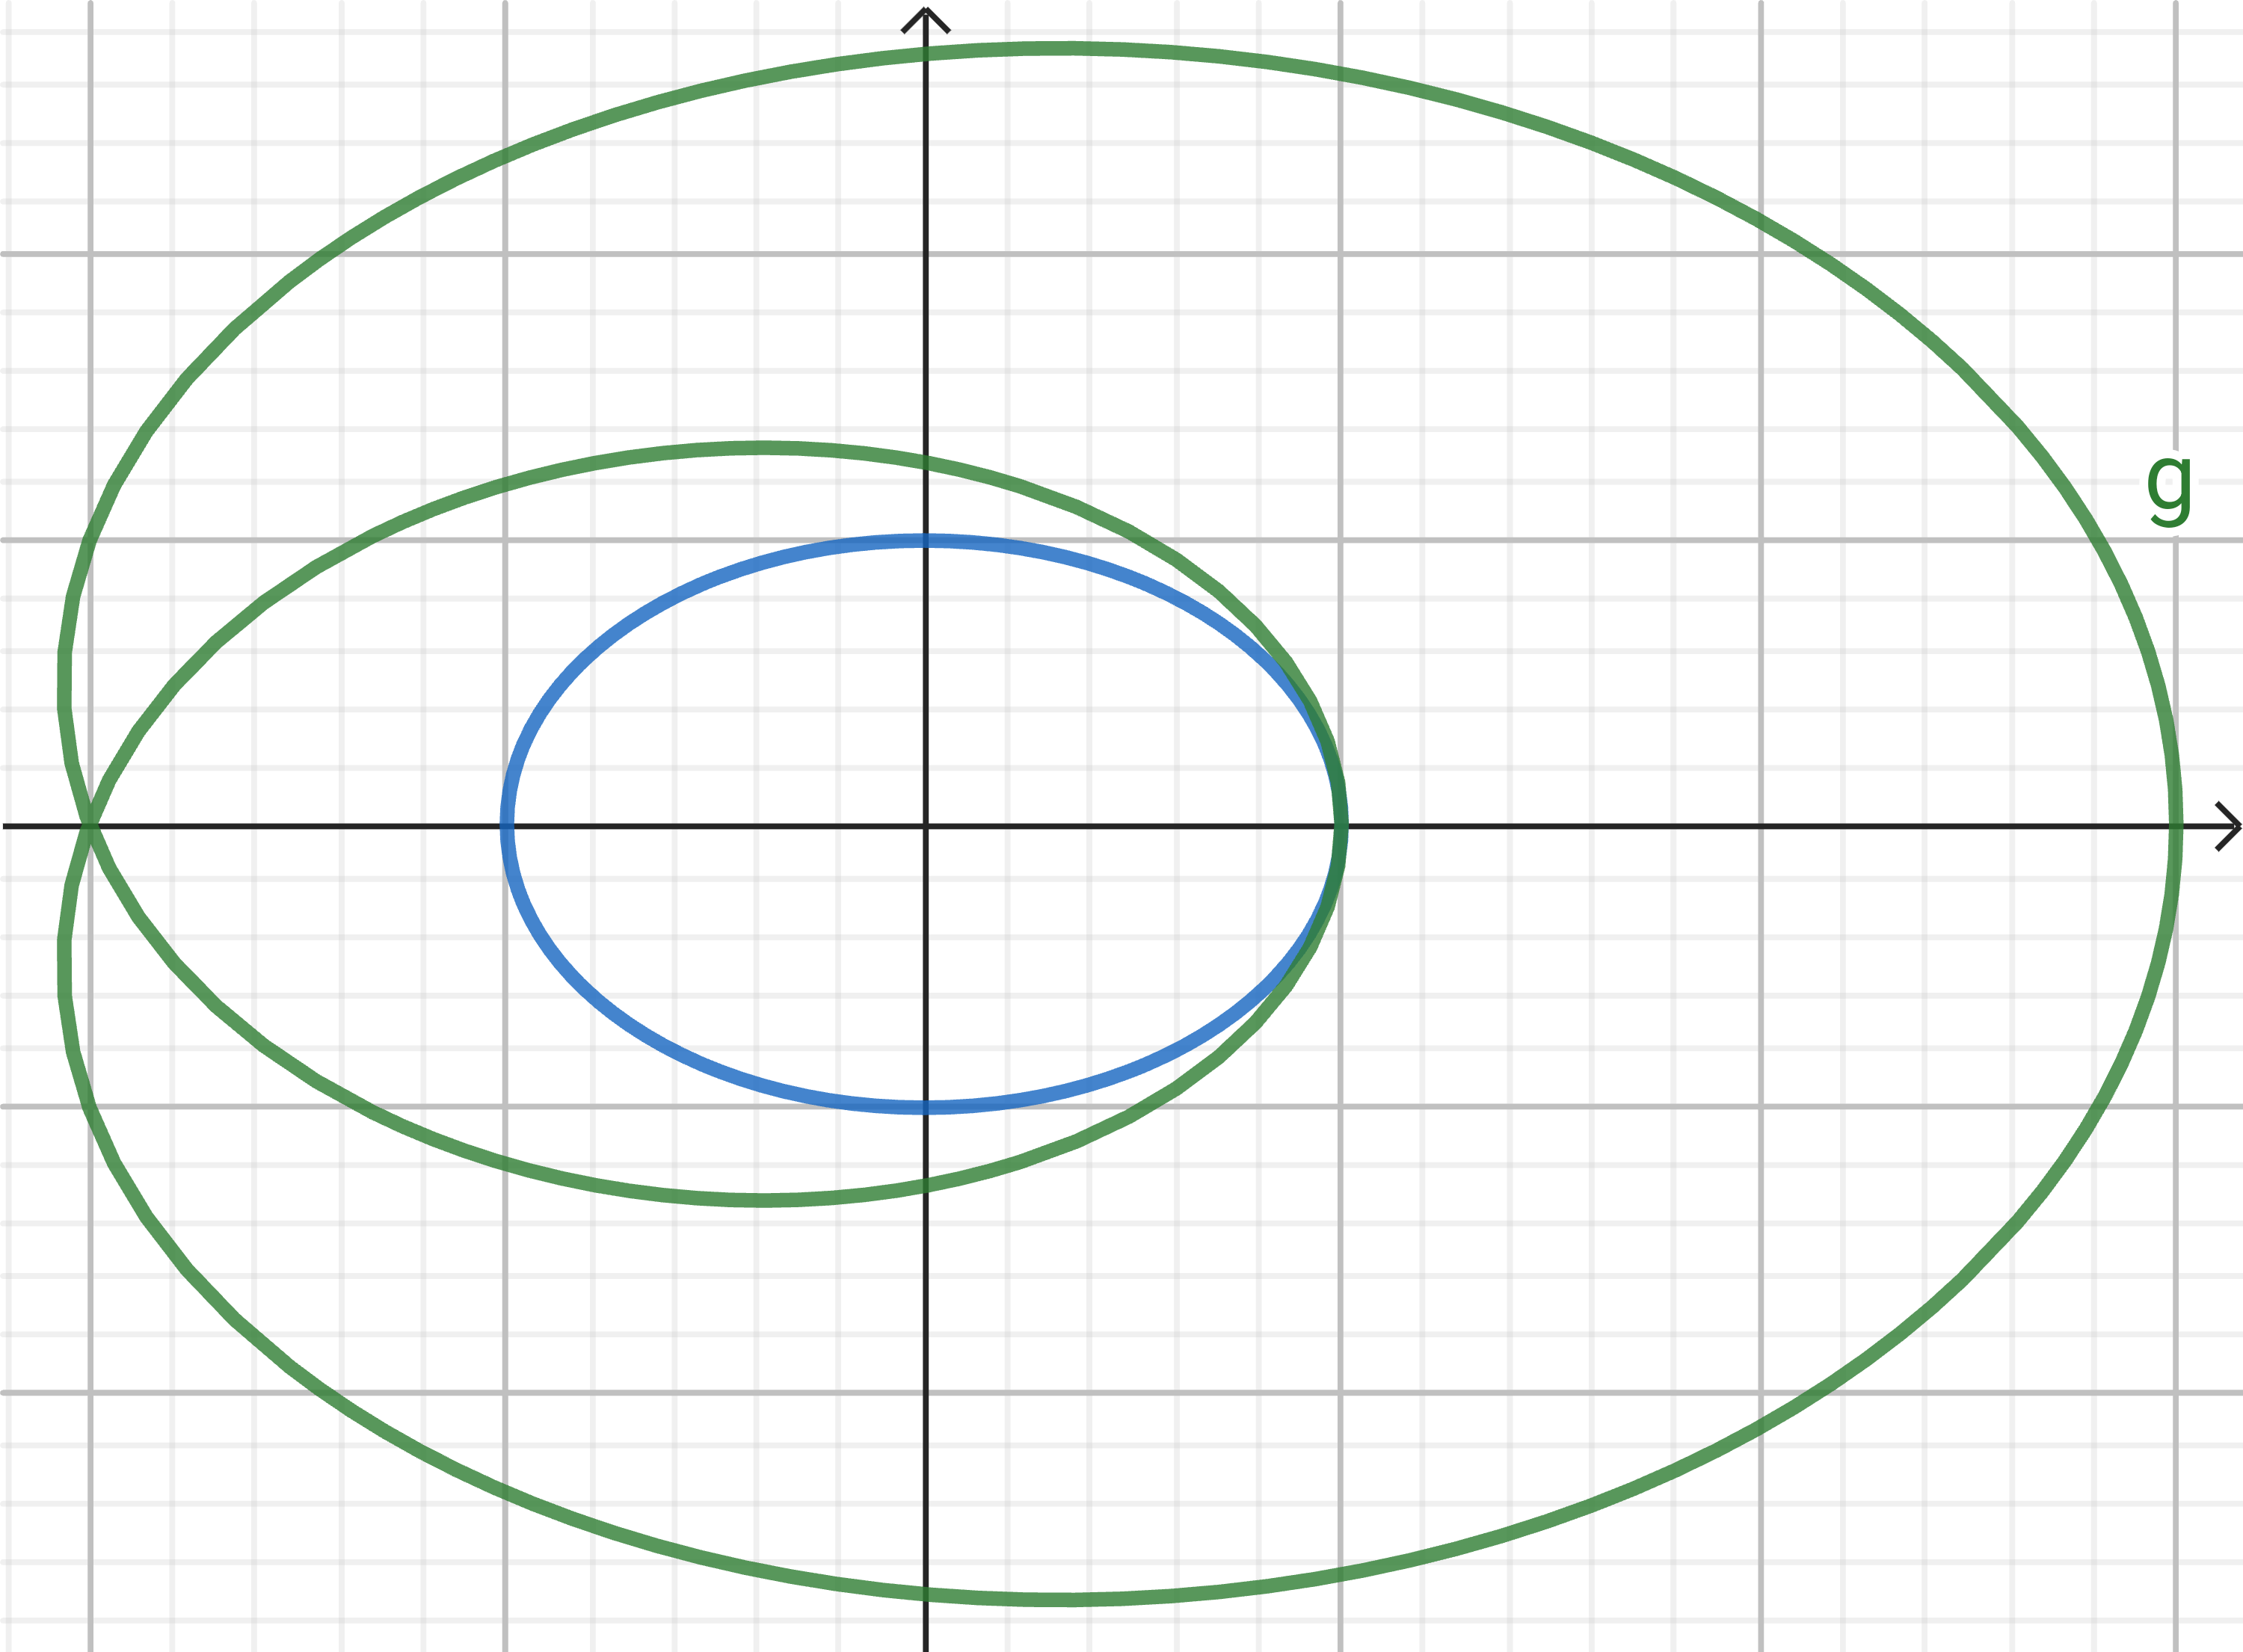
\includegraphics[width = 5cm]{conteudo/homotopia.png}
\end{figure}

\begin{titlemize}{Lista de consequências}
	\item \hyperref[teo-fundamental-da-algebra]{teo-fundamental-da-algebra};\\ 
	
\end{titlemize}

\subsection{teo-fundamental-da-algebra} %afirmação aqui significa teorema/proposição/colorário/lema
\label{teo-fundamental-da-algebra}
\begin{titlemize}{Lista de dependências}
	\item \hyperref[lema-teo-fundamental-da-algebra]{lema-teo-fundamental-da-algebra};\\ %'dependencia1' é o label onde o conceito Dependência 1 aparece (--à arrumar um padrão para referencias e labels--) 
	\item \hyperref[extensão-de-função-na-esfera]{extensão-de-função-na-esfera};\\
  \item \hyperref[grupo-fundamental-de-S1-prop]{grupo-fundamental-de-S1-prop}
\end{titlemize}
\begin{thm}[Teorema Fundamental da Álgebra]

	Todo polinômio não constante com coeficientes complexos possui raíz em $\mathbb{C}$. \\
 
 Em outras palavras, esse teorema garante que o corpo dos complexos é um fecho algébrico dos corpos de característica 0.
 
\end{thm}

\begin{dem}

Pelo lema referenciado na lista de dependências, basta mostrar que as funções $f_r^n: r\mathbb{S}^1 \rightarrow \mathbb{C}\backslash\{0\}$, definidas por $f_r^n(z) = z^n$, não são homotópicas a uma constante.
De fato, caso $f_r^n$ fosse homotópica a uma constante, então $h: \mathbb{S}^1 \rightarrow r\mathbb{S}^1 \rightarrow \mathbb{C}\backslash\{0\} \rightarrow \mathbb{S}^1$ dada por $h(z) = \frac{f_r^n(rz)}{|f_r^n(rz)|}$ também seria homotópica a uma constante, já que se $H:r\mathbb{S}^1 \times I \rightarrow \mathbb{C}\backslash\{0\}$ é a homotopia entre $f_r^n$ e uma constante $c_0$, então $\frac{1}{r^n}H(rz, t)$ é homotopia entre $h$ e $\frac{c_0}{r^n}$.\\
No entanto, por uma das equivalências de \hyperref[extensão-da-função-na-esfera]{extensão-da-função-na-esfera}, se $h$ é homotópica a uma constante, então $h_*$ é trivial, implicando que $h_*([e^{2\pi i}])$ é elemento neutro em $\mathcal{S}^1$, ou seja $[e^{2\pi in}] = [1]$ e, portanto, com a linguagem do levantamento de homotopia na seção do grupo fundamental de $\mathbb{S}^1$, temos que $deg([e^{2\pi in]}) = deg([1]) = 0$, contrariando o fato de que, na verdade, $deg([e^{2\pi in}]) = n$. Portanto, $f_r^n$ não pode ser homotópico a uma constante e, dessa forma, vale o Teorema Fundamental da Álgebra.

    
\end{dem}

Note que a interpretação geométrica de $h$ é de alongar os pontos em $\mathbb{S}^1$, aumentando o seu raio, e depois rotacioná-los e contraí-los de volta a $\mathbb{S}^1$. A homotopia de $h$ à constante deforma continuamente a circunferência de raio $1$ no ponto $c_0$, trazendo-o mais próximo da origem.

%---------------------------------------------------------------------------------------------------------------------!Draft!-----------------------------------------------------------------------------------------------------------------
\subsection{Identidade e antípoda são homotópicas se há campo não nulo} %afirmação aqui significa teorema/proposição/colorário/lema
\label{identidade-e-antipoda-homotopicas-prop}
\begin{titlemize}{Lista de dependências}
	\item \hyperref[homotopia-def]{Homotopia};\\ %'dependencia1' é o label onde o conceito Dependência 1 aparece (--à arrumar um padrão para referencias e labels--) 
	%\item \hyperref[]{};\\
% quantas dependências forem necessárias.
\end{titlemize}




\begin{lemma}[Funções identidade e antípoda na esfera]% ou af(afirmação)/prop(proposição)/corol(corolário)/lemma(lema)/outros ambientes devem ser definidos no preambulo de Alg.Top-Wiki.tex 
	Se existe uma função contínua $v:S^n\rightarrow \mathbb{R}^{n+1}$ que leva todo $x\in S^n$ em $v(x)$ com $\langle x, v(x) \rangle =0$, isto é, um campo vetorial contínuo não nulo tangente à esfera, então as funções identidade $Id_{S^n}:S^n\rightarrow S^n$ e antípoda $A_{S^n}:S^n\rightarrow S^n$ dada por $A_{S^n}(x)=-x$ para todo $x\in S^n$ são homotópicas.
\end{lemma}
\begin{dem}
    Seja $v:S^n\rightarrow \mathbb{R}^{n+1}$ o campo vetorial contínuo tangente à esfera que é não nulo em todos os pontos e considere a função contínua $H:S^n\times I\rightarrow S^n$ definida por $$H(x,t)=cos(\pi t)x+sen(\pi t)\frac{v(x)}{||v(x)||}.$$
    De fato, $H$ está bem definida pois, utilizando o fato de que $\langle x, v(x) \rangle =0$, temos 

    $$|cos(\pi t)x+sen(\pi t)\frac{v(x)}{||v(x)||}|^2=$$$$=\langle cos(\pi t)x+sen(\pi t)\frac{v(x)}{||v(x)||} , cos(\pi t)x+sen(\pi t)\frac{v(x)}{||v(x)||}\rangle=$$$$=cos^2(\pi t)\langle x,x \rangle +sen^2(\pi t)\langle \frac{v(x)}{||v(x)||},\frac{v(x)}{||v(x)||}\rangle=$$$$=cos^2(\pi t)+sen^2(\pi t)=1.$$
    
    Isto é, $H(x,t)$ pertence à esfera para todo $(x,t)\in X\times I$. Além disso, $H$ é homotopia entre a identidade e a antípoda pois $$H(x,0)=cos(0)x+sen(0)\frac{v(x)}{||v(x)||}=x=Id(x)\text{ para todo } x\in S^n$$ $$\text{e } H(x,1)=cos(\pi)x+sen(\pi)\frac{v(x)}{||v(x)||}=-x=A(x)\text{ para todo }x\in S^n.$$
\end{dem}


\begin{titlemize}{Lista de consequências}
	\item \hyperref[teorema-bola-cabeluda-prop]{Teorema da Bola Cabeluda};\\ %'consequencia1' é o label onde o conceito Consequência 1 aparece
	%\item \hyperref[]{}
\end{titlemize}

%[Bianca]: Um arquivo tex pode ter mais de uma afirmação (ou definição, ou exemplo), mas nesse caso cada afirmação deve ter seu próprio label. Dar preferência para agrupar afirmações que dependam entre sí de maneira próxima (um teorema e seu corolário, por exemplo)

%---------------------------------------------------------------------------------------------------------------------!Draft!-----------------------------------------------------------------------------------------------------------------
\subsection{Teorema da Bola Cabeluda} %afirmação aqui significa teorema/proposição/colorário/lema
\label{teorema-bola-cabeluda-prop}
\begin{titlemize}{Lista de dependências}
	\item \hyperref[homotopia-def]{Homotopia};\\ %'dependencia1' é o label onde o conceito Dependência 1 aparece (--à arrumar um padrão para referencias e labels--) 
	\item \hyperref[identidade-e-antipoda-homotopicas-prop]{Homotopia entre identidade e antípoda};\\
% quantas dependências forem necessárias.
\end{titlemize}


\begin{thm}[Teorema da Bola Cabeluda]% ou af(afirmação)/prop(proposição)/corol(corolário)/lemma(lema)/outros ambientes devem ser definidos no preambulo de Alg.Top-Wiki.tex 
	A esfera $S^n$ possui um campo vetorial contínuo não nulo em todo ponto isto é, existe uma função contínua $v:S^n\rightarrow \mathbb{R}^{n+1}$ que leva todo $x\in S^n$ a $v(x)$ com $\langle x, v(x) \rangle =0$ e $v(x)\ne 0$, se e somente se $n$ é ímpar.\\
\end{thm}
\begin{dem}
    Se $n$ é ímpar, $n=2k-1$ para algum natural $k$ e basta tomar o campo $$v(x_1,~...,~x_{2k})=(-x_2,~x_1,~-x_4,~x_3,~...,~-x_{2k},~x_{2k-1})\text{ para todo }(x_1,~...,~x_{2k})\in S^n.$$
    De fato, a função é contínua, temos $$\langle(-x_2,~x_1,~...,~-x_{2k},~x_{2k-1}), (x_1,~x_2,~...,~x_{2k-1},~x_{2k}) \rangle =$$$$=-x_1x_2+x_1x_2-...-x_{2k-1}x_{2k}+x_{2k-1}x_{2k}=0$$ e vale $v(x)\ne 0$ para todo $x=(x_1,...,x_{2k})\in S^n$ pois $v(x)=(x_1,~x_2,~...,~x_{2k-1},~x_{2k})=0$ somente se $x_i=0$ para todo $i\in {1,~...,~2k}$, isto é, $v(x)=0$ apenas em ponto fora da esfera.\\

    Reciprocamente, se a esfera $S^n$ possui campo vetorial contínuo não nulo em cada ponto conforme condição do enunciado, segundo o lema \ref{identidade-e-antipoda-homotopicas-prop}, existe uma homotopia entre os mapas identidade e antípoda na esfera, o que não pode ocorrer de $n$ for par.

    
\end{dem}

Vale ressaltar que é possível demostrar que de fato não há homotopia entre a identidade e a antípoda em esferas de grau par através da noção de grau de uma função, existente em homologia. Esse tópico não será abordado neste material.

\begin{titlemize}{Lista de consequências}
	\item \hyperref[consequencia1]{Consequência 1};\\ %'consequencia1' é o label onde o conceito Consequência 1 aparece
	%\item \hyperref[]{}
\end{titlemize}

%[Bianca]: Um arquivo tex pode ter mais de uma afirmação (ou definição, ou exemplo), mas nesse caso cada afirmação deve ter seu próprio label. Dar preferência para agrupar afirmações que dependam entre sí de maneira próxima (um teorema e seu corolário, por exemplo)
%%% Local Variables:
%%% mode: LaTeX
%%% TeX-master: "../Alg.Top-Wiki"
%%% End:

\section{Grupo Fundamental}
\label{grupo-fundamental}

\begin{titlemize}{Lista de Dependências}
	\item \hyperref[homotopia]{Homotopia}\\ %homotopia
\end{titlemize}

Considere um espaço topológico com um ponto base fixado. O seu grupo fundamental é o grupo das classes de equivalência (sob homotopia relativa aos extremos) dos laços no espaço saindo do ponto base. Tal grupo armazena certas informações sobre buracos do espaço topologico, e é invariante sobre a equivalência homotópica. Esta é uma ferramenta poderosa para verificar se dois espaços topológicos são homeomorfos. % (homotópicos). %retirei, não entendi o que querem dizer
Veremos como sua construção se dá com mais detalhes.

%---------------------------------------------------------------------------------------------------------------------!Draft!-----------------------------------------------------------------------------------------------------------------
\subsection{Espaço de Laços}
\label{espaco-lacos-def}
\begin{titlemize}{Lista de dependências}
	%\item \hyperref[dependecia1]{Dependência 1};\\ %'dependencia1' é o label onde o conceito Dependência 1 aparece (--à arrumar um padrão para referencias e labels--)
    \item \hyperref[homotopia-relativa-def]{Homotopia Relativa}
	\item \hyperref[homotopia-relaçao-de-equivalencia-prop]{Homotopia é relação de equivalência};\\
% quantas dependências forem necessárias.
\end{titlemize}
\begin{defi}[Espaço de Laços]
	Seja $X$ um espaço topológico e seja $x_0\in X$ um ponto base. O \textbf{espaço de laços} em $X$ que saem de $x_0$ é definido como
\[\Omega(X,x_0) = \left\{\gamma: I \to X ~|~ \gamma\text{ é contínua e }\gamma(0)=\gamma(1)=x_0\right\}.\]
\end{defi}

Investigaremos a fundo o conjunto $\pi_1(X,x_0) = \Omega(X,x_0)/\sim$, onde $\alpha \sim \beta$ se, e somente se, $\alpha$ e $\beta$ são homotópicas relativo a $\partial I = \{0,1\}$.


\begin{titlemize}{Lista de consequências}
	\item \hyperref[homotopia-relaçao-de-equivalencia-prop]{Homotopia como relação de equivalência};\\ %'consequencia1' é o label onde o conceito Consequência 1 aparece
	\item \hyperref[teorema-bola-cabeluda-prop]{Teorema da bola cabeluda}
\end{titlemize}

%[Bianca]: é mais fácil criar a lista de dependências do que a de consequências.

\input{conteudo/produto-concatenacao-def}
\input{conteudo/produto-bem-definido-gr-fundamental-prop}
\subsection{Grupo fundamental}
\label{grupo-fundamental-def}
\begin{titlemize}{Lista de dependências}
	\item \hyperref[espaco-lacos-def]{O espaço de laços}
	\item \hyperref[produto-bem-definido-prop]{O produto do grupo fundamental};\\ %'dependencia1' é o label onde o conceito Dependência 1 aparece (--à arrumar um padrão para referencias e labels--) 
% quantas dependências forem necessárias.
\end{titlemize}
\begin{defi}[Grupo fundamental]
    Seja $X$ um espaço topológico e seja $x_0$ um ponto de $X.$ \textbf{O grupo fundamental de} $X$ em $x_0$ é $(\pi_1(X,x_0),\cdot)$, onde $\pi_1(X,x_0) = \Omega(X,x_0)/\sim$, onde $\alpha \sim \beta$ se, e somente se, $\alpha$ e $\beta$ são homotópicas relativo aos extremos, e o produto $\cdot$ é dado por $[\alpha]\cdot[\beta] = [\alpha \ast \beta]$, em que $\alpha \ast \beta$ é a concatenação de $\alpha$ e $\beta$.
\end{defi}

No geral, o grupo fundamental depende da escolha do ponto base $x_0$. A seguir, apresentamos um exemplo elementar de grupo fundamental.
\begin{ex}
    Seja $X=\{x\}$ é um espaço topológico contendo apenas um ponto. Nesse caso, o único laço em $X$ é a função constante $c_x:I\rightarrow \{x\}$. Assim, a única classe de homotopia é $[c_x]$, o que implica que $\pi_1(\{x\},x)=0$.
\end{ex}

\begin{titlemize}{Lista de consequências}
	\item \hyperref[hom-grupo-fundamental]{Homomorfismo de grupos fundamentais};%'consequencia1' é o label onde o conceito Consequência 1 aparece
	%\item \hyperref[]{}
\end{titlemize}

\input{conteudo/homomorfismo-de-grupo-fundamental-prop}
%---------------------------------------------------------------------------------------------------------------------!Draft!-----------------------------------------------------------------------------------------------------------------
\subsection{Conjugação por uma Curva} %[conjugacao-por-curva-prop]{Conjugação por uma Curva}
\label{conjugacao-por-curva-prop}
\begin{titlemize}{Lista de dependências}
    \item \hyperref[espaco-lacos-def]{Espaço de Laços};\\
    \item \hyperref[produto-bem-definido-prop]{O produto do grupo fundamental};\\
	\item \hyperref[grupo-fundamental-def]{O Grupo Fundamental};
% quantas dependências forem necessárias.
\end{titlemize}
%Comentário sobre os objetos envolvidos na afirmação.
\begin{defi}[Conjugação de laços por uma curva] 
	Sejam $x_0$ e $x_1$ pontos em um espaço topológico $X$ e seja $\gamma: I \to X$ uma curva contínua ligando $x_0$ a $x_1$; isto é, $\gamma(0)=x_0$ e $\gamma(1) = x_1$. Seja também $\eta \in \Omega(X,x_0)$ um laço saindo de $x_0$. Definimos a conjugação de $\eta$ por $\gamma$ como $\overline{\gamma} * \eta * \gamma \in \Omega(X,x_1)$, laço saindo de $x_1$. Isto define uma função $A_{\gamma}: \Omega(X,x_0) \to \Omega(X,x_1)$.
\end{defi}

\begin{prop}[Isomorfismo de grupos induzido por $A_{\gamma}$]
    Sejam $x_0$ e $x_1$ pontos em um espaço topológico $X$ e seja $\gamma: I \to X$ uma curva ligando $x_0$ a $x_1$.
    
    Então $A_{\gamma}$ induz um isomorfismo de grupos \begin{align*}
        \hat{A}_{\gamma}: \pi_1(X,x_0)&\to \pi_1(X,x_1)\\
        \hat{A}_{\gamma}([\eta]) &= [A_{\gamma}(\eta)] = [\overline{\gamma} * \eta * \gamma].
    \end{align*}

    \begin{dem}
        Provemos primeiramente que $\hat{A}_{\gamma}$ está bem definida. Considere $c_{\gamma}: \gamma \Rightarrow \gamma$ e $c_{\overline{\gamma}}: \overline{\gamma} \Rightarrow \overline{\gamma}$ as homotopias constantes. Assim, se $\eta, \nu \in \Omega(X,x_0)$ e $H: \eta \Rightarrow \nu$ é uma homotopia relativa a $\partial I$ então é claro que $c_{\overline{\gamma}}*H*c_{\gamma}: A_{\gamma}(\eta) \Rightarrow A_{\gamma}(\nu)$ também é homotopia relativa a $\partial I$.

        $\hat{A}_{\gamma}$ é um homomorfismo de grupos, já que dadas $\eta, \nu \in \Omega(X,x_0)$,
        \begin{align*}
            \hat{A}_{\gamma}([\eta]\cdot[\nu]^{-1})
            &= \hat{A}_{\gamma}([\eta * \overline{\nu}])\\
            &= [\overline{\gamma} * (\eta * \overline{\nu}) * \gamma]\\
            &= [(\overline{\gamma} * \eta * \gamma)*(\overline{\gamma} * \overline{\nu} * \gamma)]\\
            &= [\overline{\gamma} * \eta * \gamma]\cdot[\overline{\overline{\gamma} * \nu * \gamma}]\\
            &= \hat{A}_{\gamma}([\eta]) \cdot \hat{A}_{\gamma}([\nu])^{-1}.
        \end{align*}
        
        Por fim, note que $\hat{A}_{\gamma}$ e $\hat{A}_{\overline{\gamma}}$ são inversas, pois \[A_{\gamma} \circ A_{\overline{\gamma}}(\eta) = (\overline{\gamma} * \gamma) * \eta * (\overline{\gamma} * \gamma) \sim \eta\text{ relativa a }\partial I\]
        para toda curva $\gamma: I \to X$. Desse modo $\hat{A}_{\gamma}$ é um isomorfismo de grupos.
    \end{dem}
\end{prop}

Um fato importante decorrente de tal proposição é o seguinte.

\begin{corol}
    Se $X$ é um espaço topológico então $\pi_1(X,x_0)$ é isomorfo a $\pi_1(X,x_1)$, para quaisquer $x_0, x_1 \in X$ na mesma componente conexa por caminhos de $X$. Em especial, o grupo fundamental independe do ponto base caso $X$ seja conexo por caminhos.
\end{corol}

Dessa forma, se $X$ é um espaço conexo por caminhos, podemos denotar o grupo fundamental de $X$ por $\pi_1(X)$, omitindo o ponto base.

\begin{nota}
    Sejam $X$ e $Y$ espaços topológicos, $x_0, x_1\in X$ e $\gamma:I\to X$ uma curva ligando $x_0$ a $x_1$. Seja também $f: X\to Y$ uma função contínua e denotemos $y_0 = f(x_0)$ e $y_1 = f(x_1)$. Então $f(\gamma):I \to Y$ liga $y_0$ a $y_1$, e vale que
    \[f_{*,x_1} \circ \hat{A}_{\gamma} = \hat{A}_{f(\gamma)} \circ f_{*,x_0}.\]
    \begin{dem}
        Para cada $\eta \in \Omega(X,x_0)$,
        \begin{align*}
            \hat{A}_{f(\gamma)} \circ f_{*,x_0}([\eta])
            &= \hat{A}_{f(\gamma)} ([f(\eta]))\\
            &= [\overline{f(\gamma)} * f(\eta) * f(\gamma)]\\
            &= [f(\overline{\gamma}) * f(\eta) * f(\gamma)]\\
            &= [f(\overline{\gamma} * \eta * \gamma)]\\
            &= [f(A_{\gamma}(\eta)]
            = f_{*,x_1}\circ \hat{A}_{\gamma}([\eta]).
        \end{align*}
    \end{dem}
\end{nota}

\begin{titlemize}{Lista de consequências}
	\item \hyperref[equiv-homotopia-induz-iso]{Equivalência de homotopia e o grupo fundamental}%;\\ %'consequencia1' é o label onde o conceito Consequência 1 aparece
	%\item \hyperref[]{}
\end{titlemize}

%[Bianca]: Um arquivo tex pode ter mais de uma afirmação (ou definição, ou exemplo), mas nesse caso cada afirmação deve ter seu próprio label. Dar preferência para agrupar afirmações que dependam entre sí de maneira próxima (um teorema e seu corolário, por exemplo)

\input{conteudo/equivalencia-de-homotopia-induz-iso-thm}
\subsection{O Grupo Fundamental de um Espaço Convexo}
\label{grupo-fundamental-convexo}
\begin{titlemize}{Lista de dependências}
	\item \hyperref[grupo-fundamental-def]{Grupo Fundamental};\\ %'dependencia1' é o label onde o conceito Dependência 1 aparece (--à arrumar um padrão para referencias e labels--) 
% quantas dependências forem necessárias.
\end{titlemize}

\begin{ex}[Grupo fundamental de um espaço convexo]
O grupo fundamental de um espaço convexo X é sempre trivial, i.e, $\pi_1(X, x_0) = \{ 1\}$.
\end{ex}

De fato, isso se verifica pois, se $\alpha$ é um laço em um espaço topológico $X$ começando em um ponto $x_0$, tomando a homotopia $F:I \times I \longrightarrow X$, onde $F(s,t) = (1 - t)\alpha(s) + tx_0$, tem-se que $\alpha \sim c_{x_0}$. Assim, $\pi_1(X, x_0) = \{1\}$.

%\begin{figure}[]
%	\centering
%	\includegraphics[width=0.8\textwidth]{}
%	\caption{}
%	\label{fig:}
%\end{figure}


\subsection{Grupo fundamental de espaço de produtos}
\label{grupo-fundamental-de-espaco-de-produtos-prop}
\begin{titlemize}{Lista de dependências}
    \item \hyperref[homotopia-def]{Homotopia};\\
    \item \hyperref[grupo-fundamental]{Grupo fundamental};\\
    \item \hyperref[hom-grupo-fundamental]{Homomorfismo de grupos fundamentais}.
\end{titlemize}

\begin{prop}
    Sejam $X,Y$ espaços topológicos, com $x_0\in X$ e $y_0\in Y$, e sejam $p:X\times Y\rightarrow X$ e $q:X\times Y\rightarrow Y$ projeções canônicas. Então, o homomorfismo
    \begin{align*}
        ((p_*,q_*):\pi_1(X\times Y,(x_0,y_0))&\longrightarrow \pi_1 (X,x_0)\times \pi_1(Y,y_0)\\
        [\alpha]&\longmapsto ([p\circ \alpha],[q\circ \alpha]) 
    \end{align*}
    é um isomorfismo.
\end{prop}

\begin{dem}
    Como $p_*$ e $q_*$ são homomorfismos de grupos, $(p_*,q_*)$ também é um homomorfismo de grupos. Vamos agora verificar que $(p_*,q_*)$ é bijetivo.\\
    Injetividade: Note que $([c_{x_0}],[c_{y_0}])$ é a unidade de $\pi_1 (X,x_0)\times \pi_1(Y,y_0)$. Assim, se $[\alpha]\in \text{Ker}(p_*,q_*)$, então $[p\circ \alpha]=[c_{x_0}]$ e $[q\circ \alpha]=[c_{y_0}]$. Ou seja, existem homotopias relativa a $\partial I$, $H_1:p\circ\alpha \Rightarrow c_{x_0}$ e $H_2:q\circ \alpha \Rightarrow c_{y_0}$, o que implica que a função $H:(X\times Y)\times I\rightarrow X\times Y$ definida por
    \begin{align*}
        H((x,y),t):=(H_1(x,t),H_2(y,t))
    \end{align*}
    é uma homotopia relativa a $\partial I$ entre $(p\circ \alpha,q\circ\alpha)$ e $c_{(x_0,y_0)}$. Assim, concluímos que $[\alpha]=[c_{(x_0,y_0)}]$, o que implica que $(p_*,q_*)$ é injetivo.\\
    Sobrejetividade: Sejam $(\alpha,\beta)\in \Omega(X,x_0)\times \Omega(Y,y_0)$. Basta mostrar que existe um $\gamma\in \Omega(X\times Y,(x_0,y_0))$ tal que $p\circ\gamma=\alpha$ e $q\circ \gamma=\beta$. Porém, o laço $(\alpha,\beta)$ satisfaz exatamente essa condição. Portanto, concluímos que $(p_*,q_*)$ é sobrejetivo.
\end{dem}



%%% Local Variables:
%%% mode: LaTeX
%%% TeX-master: "../Alg.Top-Wiki"
%%% End:

\section{Espaço de recobrimento}
\label{espaco-de-recobrimento}

\begin{titlemize}{Lista de Dependências}
	\item \hyperref[homotopia]{Homotopia};\\ %homotopia
	\item \hyperref[grupo-fundamental]{Grupo fundamental};\\
    \item \hyperref[topologia-quociente]{Espaço quciente};
\end{titlemize}

Na topologia algébrica, espaços de recobrimento estão intimamente relacionados ao grupo fundamental: Todos os recobrimentos têm a propriedade de levantamento de curva e homotopia, portanto ao invés de acha uma homotopia em espaço original podemos verificar se existir uma homotopia num recobrimento que têm melhores propriedades topológicas. Por isso, os espaços de recobrimento são uma ferramenta importante no cálculo de grupos fundamentais.
\subsection{Espaço de recobrimento}
\label{espaco-de-recobrimento-def}
\begin{titlemize}{Lista de dependências}
	\item \hyperref[topologia-quociente]{Espaço quciente};\\ %'dependencia1' é o label onde o conceito Dependência 1 aparece (--à arrumar um padrão para referencias e labels--) 
% quantas dependências forem necessárias.
\end{titlemize}
\begin{defi}[Espaço de recobrimento]
Uma função contínua $p:E\rightarrow X$ é um \textbf{recobrimento} se para todo $x\in X,$ existe uma vizinhança aberta $U\subseteq X$ de $x$ e um conjunto de índices $\Lambda\ne \varnothing$ tal que 
$$p^{-1}(U)=\amalg_{\lambda\in \Lambda} V_\lambda,$$
onde $V_\lambda\subseteq E$ é um subconjunto aberto e $p|_{V_\lambda}:V_\lambda\rightarrow U$ é homeomorfismo.
\end{defi}

\begin{nota}
Introduzimos algumas terminologias: 
    \begin{itemize}
        \item $E$ é um espaço (total) de recobrimento.
        \item $U$ é um aberto uniformemente recoberto de $X.$
        \item $V_\lambda$ é uma placa de $U$ do recobrimento.
        \item A cardinalidade de $\Lambda$ é o número de folhas do recobrimento (veremos que $\# \Lambda$ não depende de $x$). 
    \end{itemize}
\end{nota}

\begin{ex}
A função $p:\mathbb{R}\rightarrow \mathbb{S}^1$ dada por $p(x)=e^{2\pi ix}$ é um recobrimento: dado $y_0=e^{2\pi i x_0}\in\mathbb{S}^1,$ e $U=\mathbb{S}^1\setminus \{-y_0\}$ nós temos 
$$p^{-1}(U)=\amalg_{k\in \mathbb{Z}} (x_0+\frac{2k-1}{2},x_0+\frac{2k+1}{2}),$$
denotamos intervalo aberto $(x_0+\frac{2k-1}{2},x_0+\frac{2k+1}{2})$ por $V_k.$ Logo, a função $p|_{V_k}:V_k\rightarrow \mathbb{S}^1\setminus\{-y\}$ é um homeomorfismo.
\end{ex}

\begin{ex}
    A função $p:\mathbb{S}^n\rightarrow \mathbb{RP}^n=\mathbb{S}^n/\mathbb{Z}_2$ dada por $p(x)=[x]$ é um recobrimento.
\end{ex}

\begin{ex}
    Dado um conjunto $\Lambda\ne \varnothing$ qualquer munido com a topologia discreta, a função projeção $pr_2:E=\Lambda\times X\rightarrow X$ é um recobrimento. Esse recobrimento é dito \textbf{recobrimento trivial}
\end{ex}

\begin{prop}
    Suponha que $X$ é um espaço topológico conexo e $p:E\rightarrow X$ um recobrimento, então toda fibra tem a mesma cardinalidade, i.e. $\# p^{-1}(x_0)=\# p^{-1}(x_1)$ para todo $x_0,\;x_1\in X.$ Isso mostra que $\Lambda$ não depende de $x$.
\end{prop}

\begin{dem}
    Seja $x_0\in X$ e seja $A=\{x_1\in X: \#p^{-1}(x_1)=\# p^{-1}(x_0)\}.$ O conjunto $A$ não é vazio, pois $x_0\in A.$ Agora vamos provar que $A$ é aberto. Suponha que $x\in A$ e seja $U$ uma vizinhança aberta de $x$ tal que $p^{-1}(U)=\amalg_{\lambda\in \Lambda} V_\lambda$ com $p|_{V_\lambda}:V_\lambda\rightarrow U$ hemeomorfismo. Então, $U\subseteq A,$ pois se $x'\in U,$ então 
    $$\# p^{-1}(x')=\# \Lambda=\# p^{-1}(x)=\# p^{-1}(x_0).$$
    O conjunto $A$ é fechado, pois $X\setminus A$ é aberto pelo mesmo argumento acima. Como $X$ é conexo, $X=A$ como queríamos. 
\end{dem}

\begin{nota}
    Localmente todo recobrimento $p:E\rightarrow U$ é isomorfo ao recobrimento trivial, i.e. para todo $x\in X,$ existem uma vizinhança aberta $U$ de $x$, um espaço topológico discreto $\Lambda,$ e um homeomorfismo $h: E|_U\rightarrow U\times \Lambda$ tal que $pr_1\circ h= p.$
\end{nota}

\begin{titlemize}{Lista de consequências}
	\item \hyperref[levantamento-de-caminhos-prop]{Levantamento de caminhos};\\ %'consequencia1' é o label onde o conceito Consequência 1 aparece
	\item \hyperref[levantamento-de-homotopia-prop]{Levantamento de homotopia}
\end{titlemize}

\input{conteudo/levantamento-de-caminhos-prop}
\subsection{Levantamento de Homotopia} %afirmação aqui significa teorema/proposição/colorário/lema
\label{levantamento-de-homotopia-prop}
\begin{titlemize}{Lista de dependências}
	\item \hyperref[espaco-de-recobrimento-def]{Espaço de recobrimento};\\ %'dependencia1' é o label onde o conceito Dependência 1 aparece (--à arrumar um padrão para referencias e labels--) 
	\item \hyperref[homotopia]{Homotopia};\\
    \item \hyperref[grupo-fundamental]{Grupo fundamental}\\
    \item \hyperref[levantamento-de-caminhos-prop]{Levantamento de caminhos}
% quantas dependências forem necessárias.
\end{titlemize}

\begin{thm}[Levantamento de Homotopia]% ou af(afirmação)/prop(proposição)/corol(corolário)/lemma(lema)/outros ambientes devem ser definidos no preambulo de Alg.Top-Wiki.tex 
	Seja $p:E\rightarrow X$ um recobrimento, e seja $H:I\times I\rightarrow X$ uma homotopia tal que $H(s,0)=\gamma:I\rightarrow X.$ Suponha que $\Tilde{\gamma}:I\rightarrow E$ é um levantamento de $\gamma,$ então existe uma única homotopia $\Tilde{H}:I\times I\rightarrow E$ tal que $\Tilde{H}(s,0)=\Tilde{\gamma}$ e $p\circ \Tilde{H}=H.$
\end{thm}

\begin{dem}
    Note que para cada $s\in I$ fixo, $\alpha^s(t):=H(s,t)$ é uma curva, logo existe um único levantamento $\tilde{\alpha}_{\tilde{\gamma}(s)}(t)$ que começa em ponto $\tilde{\gamma}(s).$ Definimos $\Tilde{H}(s,t):=\Tilde{\alpha}_{\tilde{\gamma}}(t),$ é claro que 
\[p\circ\tilde{H}(s,t)=\alpha^s (t)=H(s,t)\]
e 
\[\tilde{H}(s,0)=\Tilde{\alpha}_{\tilde{\gamma}}(0)=\tilde{\gamma}(s).\]
A unicidade segue que da unicidade do levantamento de caminhos. Pela definição de recobrimento, para cada $(s_0,t_0)\in I\times I$ existe um aberto uniformemente recoberto $U$ contendo $H(s_0,t_0)$ tal que $\tilde{H}|_M=p|_V^{-1}\circ H|_M,$ onde $V$ é uma placa de $U$ e $M=H^{-1}(U).$ Como $H$ e $p|_V^{-1}$ são contínuas e $M$ é aberto, $\tilde{H}$ é localmente contínua, e portanto contínua.
\end{dem}

\begin{corol}
    Sejam $\alpha,\;\beta:I\rightarrow X$ duas curvas. Então, $\alpha$ e $\beta$ são homotópicas relativa a $\partial I$ se, e somente se, os levantamentos $\Tilde{\alpha}_{e_0}$ e $\Tilde{\beta}_{e_0}$ são homotópicos relativo a $\partial I.$ 
\end{corol}

\begin{dem}
    Assuma que $\Tilde{H}$ é homotopia relativa a $\partial I$ dos levantamentos, então $p\circ\Tilde{H}$ é uma homotopia relativa a $\partial I.$ Vamos mostrar a recíproca. Seja $H:\alpha\Rightarrow \beta$ uma homotopia relativa a $\partial I$ e seja $\Tilde{H}:I\times I\rightarrow E$ levantamento de $H$. Temos que mostra:
    \begin{enumerate}
        \item $\tilde{H}(s,1)=\tilde{\beta}_{e_0}(s)$, i.e., $\tilde{H}:\tilde{\alpha}_{e_0}\Rightarrow\tilde{\beta}_{e_0}$ é uma homotopia.
        \item $\tilde{H}(0,t)=e_0$ para todo $t\in I$ e $\tilde{H}(1,t)=\tilde{\alpha}_{e_0}(1)=\tilde{\beta}_{e_0}(1)$ para todo $t\in I,$ i.e., $\tilde{H}:\tilde{\alpha}_{e_0}\Rightarrow\tilde{\beta}_{e_0}$ é relativa a $\partial I.$
    \end{enumerate}
    Como $\tilde{H}(s,1)$ é um levantamento de $\beta$ que começa em $e_0,$ por unicidade de levantamento, $\tilde{H}(s,1)=\tilde{\beta}_{e_0}.$ Por mesmo argumento, como $\tilde{H}(0,t)$ é um levantamento da curva constante igual à $\alpha(0)$ começando em $e_0,$ $\tilde{H}(0,t)=e_0$ para todo $t\in I.$ De forma análoga, $\tilde{H}(1,t)=\tilde{\alpha}_{e_0}(1)=\tilde{\beta}_{e_0}(1)$ para todo $t\in I.$ A demonstração está completa agora. 
\end{dem}

\begin{corol}
    Seja $p:E\rightarrow X$ um recobrimento, e sejam $\alpha,\;\beta:I\rightarrow X$ duas curvas. Se $E$ é 1-conexo, então duas curvas $\alpha,\;\beta$ são homotópica relativa a $\partial I$ se, e somente se, $\tilde{\alpha}_{e_0}(1)=\tilde{\beta}_{e_0}(1).$
\end{corol}

\begin{dem}
    A demonstração segue da definição de 1-conexo.
\end{dem}

Mostraremos um corolário bem útil em calcular grupo fundamental de um espaço topológico.

\begin{corol}\label{cor:bijedeggene}
    Seja $p:E\rightarrow X$ um recobrimento. Se $E$ é 1-conexo, então para cada pontos fixos $x\in X$ e $e\in p^{-1}(x)$, a função dada por 
    \begin{align*}
        \phi:\pi_1(X,x)&\longrightarrow p^{-1}(x)\\
        [\alpha]&\longmapsto \tilde{\alpha}_{e}(1)
    \end{align*}
    é uma bijeção.
\end{corol}

\begin{dem}
    A função $\phi$ está bem definida, pois se $[\alpha]=[\beta],$ então $\tilde{\alpha}_{e}\sim \tilde{\beta}_{e}$ relativa a $\partial I,$ em particular, $\tilde{\alpha}_e(1)=\tilde{\beta}_e(1).$
    
    A função $\phi$ é injetor, pois $E$ é 1-conexo, logo se $\tilde{\alpha}_e(1)=\tilde{\beta}_e(1),$ então $\tilde{\alpha}_e \sim \tilde{\beta}_e$ relativa a $\partial I,$ isso é equivalente a $[\alpha]=[\beta]$ pelo corolário anterior.

    A função $\phi$ é sobrejetora: Dado $e'\in p^{-1}(x).$ Pela definição de 1-conexo, existe uma curva $\gamma:I\rightarrow E$ com $\gamma(0)=e$ e $\gamma(1)=e'.$ Seja $\alpha=p\circ \gamma.$ Então, por unicidade de levantamento, $\tilde{\alpha}_e=\gamma.$ Logo, $\phi([\alpha])=\tilde{\alpha}_e(1)=\gamma(1)=e'.$ 
\end{dem}

\begin{titlemize}{Lista de consequências}
	\item \hyperref[grupo-fundamental-de-espaco-projetivo-ex]{Grupo fundamental de espaço projetivo};\\ %'consequencia1' é o label onde o conceito Consequência 1 aparece
	\item \hyperref[grupo-fundamental-de-S1-prop]{Grupo fundamental de 1-esfera};\\
 	\item \hyperref[recobrimento-1-conexo-prop]{Recobrimento 1-conexo quando X slsc};\\
  	\item \hyperref[pertence-a-base-se-e-somente-se-possui-i-trivial]{Base da topologia de $X$ possui $i^*$ trivial para todos os elementos quando há recobrimento 1-conexo};\\
   	\item \hyperref[homomorfismo-induzido-por-recobrimento-prop]{Homomorfismo induzido por recobrimento é injetor};\\
    	\item \hyperref[recobrimento-1-conexo-em-bijecao-com-P(X,x)]{Recobrimento 1-conexo em bijeção com $P(X,x_0)$}
\end{titlemize}

\input{conteudo/grupo-fundamental-de-espaco-projetivo-ex}
\input{conteudo/grupo-fundamental-de-S1-prop}
\subsection{Grupo fundamental de toro}
\label{grupo-fundamental-de-toro-ex}
\begin{titlemize}{Lista de dependências}
    \item \hyperref[homotopia-def]{Homotopia};\\
    \item \hyperref[grupo-fundamental]{Grupo fundamental};\\
    \item \hyperref[hom-grupo-fundamental]{Homomorfismo de grupos fundamentais};\\
    \item \hyperref[grupo-fundamental-de-espaco-de-produtos-prop]{Grupo fundamental de espaço de produtos};\\
    \item \hyperref[grupo-fundamental-de-S1-prop]{Grupo fundamental de 1-esfera}.
    
\end{titlemize}

\begin{ex}
    Como o toro $\mathbb{T}^2$ é homeomorfo ao $\mathbb{S}^1\times\mathbb{S}^1$. Pelas proposições \ref{grupo-fundamental-de-espaco-de-produtos-prop}, \ref{hom-grupo-fundamental} e \ref{grupo-fundamental-de-S1-prop}, obtemos 
    \[\pi_1(\mathbb{T}^2)\cong \pi_1(\mathbb{S}^1)\times\pi_1(\mathbb{S}^1)\cong\mathbb{Z}\times\mathbb{Z}.\]
\end{ex}

%---------------------------------------------------------------------------------------------------------------------!Draft!-----------------------------------------------------------------------------------------------------------------
\subsection{Recobrimento 1-conexo em bijeção com $P(X,x_0)$} %afirmação aqui significa teorema/proposição/colorário/lema
\label{recobrimento-1-conexo-em-bijecao-com-P(X,x)}
\begin{titlemize}{Lista de dependências}
	\item \hyperref[espaço-1-conexo-def]{Espaço 1-conexo};\\ %'dependencia1' é o label onde o conceito Dependência 1 aparece (--à arrumar um padrão para referencias e labels--) 
    \item \hyperref[levantamento-de-caminhos-prop]{Levantamento de caminhos}\\
	\item \hyperref[levantamento-de-homotopia-prop]{Levantamento de homotopia};\\
% quantas dependências forem necessárias.
\end{titlemize}

%Comentário sobre os objetos envolvidos na afirmação.
Seja $P(X,x_0)=\{[\gamma]|~\gamma:I\rightarrow X \text{ e }\gamma(0)=x_0\}$ o conjunto das classes de homotopia relativas a $\partial I$.

\begin{prop}%[Nome da Afirmação]% ou af(afirmação)/prop(proposição)/corol(corolário)/lemma(lema)/outros ambientes devem ser definidos no preambulo de Alg.Top-Wiki.tex 
	Se $E\rightarrow X$ é um recobrimento 1-conexo, então $E$ está em bijeção com $P(X,x_0)$
\end{prop}
\begin{dem}
    Defina $\phi: P(X, x_0)\rightarrow E$ por

    $$\phi([\gamma])=\tilde{\gamma}_{e_0}(1)\text{ para todo }[\gamma]\in P(X,x_0)$$

    onde $\tilde{\gamma}_{e_0}$ é o único levantamento de $\gamma$ começando em $e_0\in p^{-1}(x_0)$ fixado.

    Verifiquemos as seguintes afirmações:

    \begin{itemize}
        \item O mapa $\phi$ está bem definido.\newline
            Se $\gamma\sim \eta (\text{rel }\partial I)$, então, por corolário presente em \ref{levantamento-de-homotopia-prop}, temos que os levantamentos que se iniciam em $e_0$ também são homotópicos. Isto é, $\tilde{\gamma}_{e_0}\sim\tilde{\eta}_{e_0}(\text{rel }\partial I)$ e, portanto, $\tilde{\gamma}_{e_0}(1)=\tilde{\eta}_{e_0}(1)$.\newline
        
        \item O mapa $\phi$ é injetor.\newline
            Se $\tilde{\gamma}_{e_0}(1)=\tilde{\eta}_{e_0}(1)$ então, como $E$ é 1-conexo, segundo outro corolário de \ref{levantamento-de-homotopia-prop}, temos que $\gamma\sim \eta (\text{rel }\partial I)$, isto é, $[\gamma]=[\eta]$.\newline
            
        \item O mapa $\phi$ é sobrejetor.\newline
            Dado $e\in E$, escolha um caminho $\alpha:I\rightarrow E$, $\alpha(0)=e_0$ e $\alpha(1)=e$. Esse caminho existe pois $E$ é conexo por caminhos. Considere $\gamma=p\circ \alpha$. Assim, $$\phi([\gamma])=\tilde{\gamma}_{e_0}(1)=\widetilde{p\circ \alpha}_{e_0}(1)=\alpha(1),$$ onde a última igualdade segue da unicidade de levantamento.
    \end{itemize}
\end{dem}

Utilizamos $\phi$ para definir uma ação do grupo fundamental $\pi_1(X,x_0)$ em $E$. Esta ação é um mapa $\alpha: \pi_1(X,x_0)\times E\rightarrow E$ definido por

$$\alpha([\gamma], e)=[\gamma]\cdot e=\phi([\gamma*\phi^{-1}(e)])$$

Se tomarmos um caminho $ \beta: I\rightarrow E$ tal que $\beta(0)=e_0$ e $\beta(1)=e$, pode-se utilizar a definição de $\phi$ para dizer que a ação acima também pode ser escrita como

$$\alpha([\gamma], e)=[\gamma]\cdot e = \widetilde{(\gamma*(p\circ \beta))}(1)$$

Uma vez que $\phi^{-1}(e)=[p\circ \beta]$, fato que pode ser notado pois $\phi$ é bijeção e $ \phi([p\circ \beta])=\beta(1)=e$.\newline

De fato, esta é uma ação pois:

\begin{itemize}
    \item $\alpha([c_{x_0}], x)=x$ para todo $x\in E.$\newline
    Isto pode ser verificado pois $\phi([c_{x_0}*\phi^{-1}(x)])$ é tal que, se $\gamma:I\rightarrow E$ liga $e_0$ a $x$, então $\phi^{-1}(x)$ é $[p\circ \gamma]$, fato já observado anteriormente. Assim, $$\phi([c_{x_0}*\phi^{-1}(x)])=\phi([c_{x_0}*(p\circ\gamma)])=\phi([p\circ \gamma])=\widetilde{p\circ \gamma}_{e_0}(1)=\gamma(1)=x,$$ e a conclusão $\widetilde{p\circ \gamma}_{e_0}(1)=\gamma(1)$ segue da unicidade do levantamento.\newline

    \item $\alpha(\gamma_1, \alpha(\gamma_2,x))=\alpha(\gamma_1*\gamma_2,x)$

    De fato, temos$$\phi([\gamma_1 * \phi^{-1}(\alpha(\gamma_2,x))])=\phi([\gamma_1*\phi^{-1}(\phi([\gamma_2*\phi^{-1}(x)]))])=$$ $$=\phi([\gamma_1*(\gamma_2*\phi^{-1}(x))])=\phi([(\gamma_1*\gamma_2)*\phi^{-1}(x)])=$$$$=[\gamma_1*\gamma_2]\cdot x=\alpha(\gamma_1*\gamma_2,x)$$
\end{itemize}





%\begin{titlemize}{Lista de consequências}
%	\item \hyperref[consequencia1]{Consequência 1};\\ %'consequencia1' é o label onde o conceito Consequência 1 aparece
%	\item \hyperref[]{}
%\end{titlemize}

%[Bianca]: Um arquivo tex pode ter mais de uma afirmação (ou definição, ou exemplo), mas nesse caso cada afirmação deve ter seu próprio label. Dar preferência para agrupar afirmações que dependam entre sí de maneira próxima (um teorema e seu corolário, por exemplo)
%---------------------------------------------------------------------------------------------------------------------!Draft!-----------------------------------------------------------------------------------------------------------------
\subsection{Base para as topologias em um recobrimento} %afirmação aqui significa teorema/proposição/colorário/lema
\label{base-para-topologias-em-recobrimento-prop}
\begin{titlemize}{Lista de dependências}
	\item \hyperref[espaco-de-recobrimento-def]{Espaço de recobrimento};\\ %'dependencia1' é o label onde o conceito Dependência 1 aparece (--à arrumar um padrão para referencias e labels--) 
	%\item \hyperref[]{};\\
% quantas dependências forem necessárias.
\end{titlemize}






\begin{prop}[Bases das topologias de domínio e contradomínio de recobrimento]% ou af(afirmação)/prop(proposição)/corol(corolário)/lemma(lema)/outros ambientes devem ser definidos no preambulo de Alg.Top-Wiki.tex 
	Se $X$ é localmente conexo por caminhos com $p:E\rightarrow X$ um recobrimento, temos que

$$\mathcal{B}=\{U|~U\subset X\text{ é uniformemente recoberto e conexo por caminhos}\}$$

é uma base para a topologia de $X$ e

$$\tilde{{\mathcal{B}}}=\{\tilde{U}|~\tilde{U}\subset E\text{ é placa de }p:E\rightarrow X\text{ sobre }U\in \mathcal{B}\}$$
é uma base para a topologia de $E$.
\end{prop}
\begin{dem}A demostração será dividida em dois itens.\newline

    $\bullet$ Verificação de que $\mathcal{B}$ é base:\newline
    
    Por $p:E\rightarrow X$ ser um recobrimento, temos que para todo $x\in X$ existe $U$ vizinhança de $x$ tal que $p^{-1}(U)=\underset{\lambda\in \Lambda}{\bigsqcup } V_\lambda$, com cada $V_\lambda$ homeomorfo a $U$.
    
    Como $X$ é localmente conexo por caminhos, existe $U'\subset U$ vizinhança de $x$ conexa por caminhos tal que $U' $ também deve ser uniformemente recoberto por ser subconjunto de um outro aberto uniformemente recoberto.\newline
    
    Detalhadamente, este fato pode ser notado por $p(V_\lambda\cap p^{-1}(U'))$ ser $$p(V_\lambda)\cap U'=U\cap U'=U',$$ isto é, como $p|_{V_\lambda}: V_\lambda \rightarrow U$ é homeomorfismo, $p|_{V_\lambda\cap p^{-1}(U')}$ também precisa ser um homeomorfismo entre $V_\lambda\cap p^{-1}(U')$ e a imagem de $p|_{V_\lambda\cap p^{-1}(U')}$, que é $U'$. Portanto, de fato $$p^{-1}(U')=\underset{\lambda\in \Lambda}{\bigsqcup } (V_\lambda \cap p^{-1}(U')) $$ onde todo $V_\lambda \cap p^{-1}(U')$ é homeomorfo a $U'$ através de $p|_{V_\lambda \cap p^{-1}(U')}$.\newline
    
    Assim, verifica-se que os abertos de $\mathcal{B}$ cobrem todo o espaço $X$.\newline

    Além disso, ao intersectar dois abertos  $U,~ V\in\mathcal{B}$, temos um novo aberto conexo por caminhos tal que $U\cap V$ é subespaço tanto de $U$ quanto de $V$, dois abertos uniformemente recobertos. Assim, como já foi mostrado anteriormente na verificação de que $U'$ era uniformemente recoberto, temos que a intersecção de elementos de $\mathcal{B}$ é uniformemente recoberta também. Portanto, $U\cap V \in \mathcal{B}$.\newline

    Com as informações acima, de fato concluí-se que $\mathcal{B}$ é base.\newline
    
%%%%%%%%%%‰‰%%%%%‰%%%%%%%%%%%%%%
    $\bullet$ Verificação de que $\tilde{\mathcal{B}}$ é base:\newline
    
    Temos que para todo $y\in E$, $p(y)\in X$ é tal que existe $U$ vizinhança conexa por caminhos de $p(y)$ que é aberto uniformemente recoberto. Este fato foi provado anteriormente, no processo de demonstração de que $\mathcal{B}$ é base para a topologia de $X$.
    
    Isso significa que $p^{-1}(U)=\underset{\lambda\in \Lambda}{\bigsqcup } V_\lambda$, com homeomorfismos $p|_{V_\lambda}: V_\lambda  \rightarrow U$ e assim, $y\in V_{\lambda_0}$ placa de $p:E\rightarrow X$ sobre $U\in \mathcal{B}$ para algum $ \lambda_0\in \Lambda.$
    Com isso, mostramos que todo ponto de $E$ está em algum aberto de $\tilde{\mathcal{B}}.$\newline


    Por fim, temos que se $V^1_{\lambda_0}$ e $V^2_{\lambda_1}$ são abertos de $\tilde{\mathcal{B}}$ que possuem intersecção não vazia, eles são tais que $$p^{-1}(U_1)=\underset{\lambda\in \Lambda}{\bigsqcup } V_\lambda^1\text{ e }p^{-1}(U_2)=\underset{\lambda\in \Lambda}{\bigsqcup } V_\lambda^2,$$ com $\lambda_0, \lambda_1 \in \Lambda$ para certos $U_1,U_2\in \mathcal{B}$. Como já visto anteriormente, a intersecção $U_1\cap U_2$ de espaços pertencentes a $\mathcal{B}$, também pertence a $\mathcal{B}$.

    Como a união de placas que formam $p^{-1}(U_1)$ e $p^{-1}(U_2)$ é disjunta, $V^1_{\lambda_0}$ e $V^2_{\lambda_1}$ possuírem intersecção não vazia significa que $V^1_{\lambda_0}\cap V^2_{\lambda_1}$ é placa de $p:E\rightarrow X$ sobre $U_1\cap U_2$. De fato:

    
    $$p^{-1}(U_1\cap U_2)=\underset{\alpha\in \Lambda, \beta \in \Lambda, V^1_\alpha \cap V^2_\beta\ne \emptyset}{\bigsqcup } (V^1_\alpha \cap V^2_\beta)\text{ com }U_1\cap U_2\in \mathcal{B}$$ como verificado no processo anterior de $\mathcal{B}$ ser base para $X$. Portanto, $V^1_{\lambda_0}\cap V^2_{\lambda_1}\in \tilde{\mathcal{B}}$, o que conclui a verificação de que $\tilde{\mathcal{B}}$ é base de $E$.
\end{dem}



\begin{titlemize}{Lista de consequências}
	\item \hyperref[descrição-da-base-do-recobrimento-prop]{Descrição de $\tilde{\mathcal{B}}$ em termos de $X$};\\ %'consequencia1' é o label onde o conceito Consequência 1 aparece
	\item \hyperref[pertence-a-base-se-e-somente-se-possui-i-trivial]{Proposição - nova descrição da base $\mathcal{B}$}
\end{titlemize}

%[Bianca]: Um arquivo tex pode ter mais de uma afirmação (ou definição, ou exemplo), mas nesse caso cada afirmação deve ter seu próprio label. Dar preferência para agrupar afirmações que dependam entre sí de maneira próxima (um teorema e seu corolário, por exemplo)








%---------------------------------------------------------------------------------------------------------------------!Draft!-----------------------------------------------------------------------------------------------------------------
\subsection{Homomorfismo induzido por recobrimento é injetor} 
\label{homomorfismo-induzido-por-recobrimento-prop} %afirmação aqui significa teorema/proposição/colorário/lema

\begin{titlemize}{Lista de dependências}
	\item \hyperref[espaco-de-recobrimento-def]{Espaço de recobrimento};\\ %'dependencia1' é o label onde o conceito Dependência 1 aparece (--à arrumar um padrão para referencias e labels--) 
	\item \hyperref[levantamento-de-homotopia-prop]{Levantamento de homotopia};\\
% quantas dependências forem necessárias.
\end{titlemize}

\begin{lemma}[Homomorfismo induzido por recobrimento é injetor]% ou af(afirmação)/prop(proposição)/corol(corolário)/lemma(lema)/outros ambientes devem ser definidos no preambulo de Alg.Top-Wiki.tex 
	O mapa $p_*:\pi_1(E, \tilde{x}_0)\rightarrow \pi_1(X, x_0)$ induzido por um espaço de recobrimento $p:(E, \tilde{x}_0)\rightarrow (X,x_0)$ é injetivo.
\end{lemma}
\begin{dem}
    Como $p_*$ é um homomorfismo de grupo, basta verificar que o núcleo é trivial.

    Um elemento no núcleo é a classe de homotopia relativa ao ponto base $\tilde{x}_0$ de algum caminho fechado $\gamma$ tal que existe homotopia entre $p(\gamma)$ e o caminho $c_{x_0}$ constante em $x_0$. Segundo Corolário presente em \ref{levantamento-de-homotopia-prop}, temos que dois caminhos em $X$ são homotópicos relativo a $\partial I$ se e somente se os levantamentos destes caminhos com início em algum $e_0\in p^{-1}(x_0) $são homotópicos. Isto é, se $p(\gamma)$ e $c_{x_0}$ são homotópicos, então $\gamma$ e $c_{\tilde{x}_0}$ são homotópicos por serem levantamentos com início em $\tilde{x}_0$ de $p(\gamma)$ e de $c_{x_0}$ respectivamente.
    
    Portanto, todo caminho $\gamma$ cuja classe está no núcleo de $p_*$ é homotópico relativo a $\partial I$ ao caminho constante $c_{x_0}$. Assim, o núcleo é trivial e concluímos que $p_*$ é mapa injetor.
\end{dem}



\begin{titlemize}{Lista de consequências}
	\item \hyperref[recobrimento-1-conexo-prop]{Recobrimento 1-conexo quando X slsc};\\ %'consequencia1' é o label onde o conceito Consequência 1 aparece
\end{titlemize}

%[Bianca]: Um arquivo tex pode ter mais de uma afirmação (ou definição, ou exemplo), mas nesse caso cada afirmação deve ter seu próprio label. Dar preferência para agrupar afirmações que dependam entre sí de maneira próxima (um teorema e seu corolário, por exemplo)

\subsection{Recobrimento 1-conexo quando X slsc} %afirmação aqui significa teorema/proposição/colorário/lema
\label{recobrimento-1-conexo-prop}
\begin{titlemize}{Lista de dependências}
    \item \hyperref[espaco-de-recobrimento-def]{Espaço de recobrimento};\\
	\item \hyperref[espaço-semi-localmente-simplesmente-conexo-def]{Espaço semi-localmente simplesmente conexo};\\ %'dependencia1' é o label onde o conceito Dependência 1 aparece (--à arrumar um padrão para referencias e labels--) 
	\item \hyperref[espaço-1-conexo-def]{Espaço 1-conexo};\\
    \item \hyperref[levantamento-de-homotopia-prop]{Levantamento de homotopia};\\
% quantas dependências forem necessárias.
\end{titlemize}

\begin{thm}[Recobrimento 1-conexo]% ou af(afirmação)/prop(proposição)/corol(corolário)/lemma(lema)/outros ambientes devem ser definidos no preambulo de Alg.Top-Wiki.tex 
	Seja $X$ um espaço conexo por caminhos e localmente conexo por caminhos. Então $X$ admite um recobrimento 1-conexo $p:E\rightarrow X$ se e somente se $X$ for semi-localmente simplesmente conexo.\\
\end{thm}
\begin{dem}
    Por um lado, se $X$ admite um recobrimento 1-conexo $p:E\rightarrow X$, isto é, com $E$ 1-conexo, temos a seguinte situação:\newline

    Sabemos que, por definição de recobrimento, para todo $x\in X$ existe $U\subset X$ vizinhança de $x$ que é uniformemente recoberto, conforme terminologia apresentada em \ref{espaco-de-recobrimento-def}.

    Assim, mostremos que, dada a inclusão $i:U\rightarrow X$, temos que $i_*:\pi(U,x)\rightarrow \pi(X,x)$ é um mapa trivial.

    Tome $[\alpha]_U \in \pi_1(U,x)$ qualquer. Denotemos $i_*([\alpha]_U)=[i\circ \alpha]$ por $[\alpha]\in \pi(X,x)$.

    Fixado $e\in E$ tal que $p(e)=x$, é possível levantar a curva $\alpha$ para $\tilde{\alpha}_e\in \Omega (E,e)$ nos termos de \ref{levantamento-de-caminhos-prop}. Assim, $\tilde{\alpha}_e$ é  curva com início em $e$. Considerando que $\alpha$ é fechada, temos que $\tilde{\alpha}_e(1)=e=c_e(1)$, onde $c_e$ é a curva constante em $e$.

    Como $E$ é 1-conexo, é possível aplicar o corolário 4 de \ref{levantamento-de-homotopia-prop}, que é aplicação direta da definição de 1-conexo, e concluir que $\tilde{\alpha}_e$ e $c_e$ são homotópicos por uma homotopia relativa a $\partial I$.
    
    Assim, $c_x$ curva constante parada no mesmo $x$ anterior em $X$, pode ser levantada a $c_e$ em $E$, enquanto $\alpha$ pode ser levantado a $\tilde{\alpha}_e$, e os levantamentos destas duas curvas são homotópicos relativamente a $\partial I$. Nesta situação, é possível aplicar o corolário 3 também de \ref{levantamento-de-homotopia-prop}, e concluir que $\alpha$ e $c_x$ são caminhos homotópicos relativamente a $\partial I$.

    Em outras palavras, $i_*[\alpha]_U=[\alpha]=[c_x]$. O que implica que $i_*$ de fato envia sempre na mesma classe e é mapa trivial.\newline\newline




    Na outra implicação, temos que se $X$ é semi-localmente simplesmente conexo:\newline
    
    A proposição \ref{recobrimento-1-conexo-em-bijecao-com-P(X,x)} é um indício de que o espaço $P(X,x_0)$ ali definido pode ser um bom candidato a espaço 1-conexo.

    De fato, iremos realizar esta verificação. 

    Lembre que $P(X,x_0)$ é definido por $\{[\gamma]| ~\gamma:I\rightarrow X\text{ ~ }\gamma(0)=x_0\}$, isto é, o espaço das classes relativas a $\partial I$ dos caminhos em $X$ que começam em $x_0$.

    Considere a projeção $q: P(X,x_0)\rightarrow X$ definida por 

    $$q([\gamma])=\gamma(1)$$

    Esta é uma função \textbf{bem definida} porque se duas curvas $\gamma_1$ e $\gamma_2$ estão na mesma classe de $P(X,x_0)$, isso significa que existe homotopia entre elas que fixa seus pontos extremos e, de fato, $q([\gamma_1])=\gamma_1(1)=\gamma_2(1)=q([\gamma_2])$.

    Além disso, $q$ é um mapa \textbf{sobrejetor} porque se $X$ é conexo por caminhos, existem curvas $\gamma$ que ligam $x_0$ a qualquer outro ponto $x\in X$. De fato, $\gamma(1)$ pode ser qualquer ponto de $X$ variando a curva.

    Considere o seguinte espaço:

    $$\mathcal{B}=\{U\subset X | U \text{ é aberto conexo por caminhos e } i^*:\pi_1(U)\rightarrow \pi_1(X)\text{ é trivial }\}$$

    Note que $i^*$ é trivial para toda escolha de ponto base em $U$, uma vez que esse aberto é conexo por caminhos. Por isso, foi escrito $\pi_1(U)$ e  $\pi_1(X)$ ao invés de  $\pi_1(U,x)$ e  $\pi_1(X,x)$ para algum $x\in U$.

    Verifiquemos que esta é uma \textbf{base para a topologia de $X$}

     Por $X$ ser semi-localmente simplesmente conexo, para todo $x\in X$ existe aberto $U$ vizinhança de $x$ tal que $i^*:\pi_1(U,x)\rightarrow \pi_1(X,x)$ é trivial. Como, além disso, $X$ é localmente conexo por caminhos, sabemos que existe $V\subset U$ conexo por caminhos que também é vizinhança de $x$. Assim, a composição dos homomorfismos induzidos por inclusões $\pi_1(V,x)\rightarrow \pi_1(U,x)\rightarrow \pi_1(X,x)$ também deve ser trivial. Dessa forma, existe $V\in \mathcal{B}$ que é vizinhança de $x$. Este argumento mostra que os abertos de $\mathcal{B}$ cobrem $X$.

     Além disso, a intersecção de quaisquer dois abertos em $\mathcal{B}$ é novamente um aberto em $\mathcal{B}$ pois a intersecção de dois abertos conexos por caminhos é um aberto conexo por caminhos. Ele será subespaço dos dois abertos iniciais e será possível construir uma composição como a do parágrafo anterior para mostrar que o homomorfismo induzido entre os grupos fundamentais da intersecção e de $X$ é trivial.

     Agora, dado um aberto $U\in \mathcal{B}$ e um caminho $\gamma:I\rightarrow X$ com $\gamma(0)=x_0$ e $\gamma(1)=x\in U$, defina por

     $$U_{[\gamma]}=\{[\gamma* \eta]\in P(X,x_0)| \eta:I\rightarrow U\text{ tal que } \eta(0)=\gamma(1)\}$$


     um aberto de $P(X,x_0)$. Note que $U_{[\gamma]}$ depende apenas da classe $\gamma$.

     Tome duas curvas quaisquer $\gamma$ e $\gamma'$ com início em $x_0$ e que terminam em algum ponto de $U\in \mathcal{B}$, como acima. Os abertos $U_{[\gamma]}$ e $U_{[\gamma']}$ são iguais se e somente se $[\gamma']\in U_{[\gamma]}$.
     
     De fato, se $U_{[\gamma]}=U_{[\gamma']}$ temos que $$[\gamma']=[\gamma'*c_{\gamma'(1)}]\in U_{[\gamma']}=U_{[\gamma]}.$$ Por outro lado, se $[\gamma']\in U_{[\gamma]}$, então $\gamma'\sim \gamma *\eta ~(\text{rel }\partial I)$ para algum $\eta$ em $U$ com início em $\gamma(1)$, o que significa que todo elemento $\varepsilon\in U_{[\gamma']}$ é tal que $$\varepsilon\sim\gamma'*\mu\sim (\gamma*\eta)*\mu (\text{rel }\partial I)$$ para algum $\mu$ em $U$ com início em $\gamma'(1)$. Isso indica que $[\varepsilon]\in U_{[\gamma]}$ e $U_{[\gamma']}\subset U_{[\gamma]}$. Além disso, todo elemento $[\epsilon] \in U_{[\gamma]}$ é tal que $$\epsilon \sim \gamma * \mu' \sim \gamma*\eta*\overline{\eta}*\mu'\sim \gamma' *\overline{\eta}*\mu'(\text{rel }\partial I)$$ e, portanto, $[\epsilon]\in U_{[\gamma']}$. Observe a situação aqui descrita na imagem \ref{fig:cobertura-P(X,x_0)} a seguir.

     \begin{figure}[h!]
         \centering
         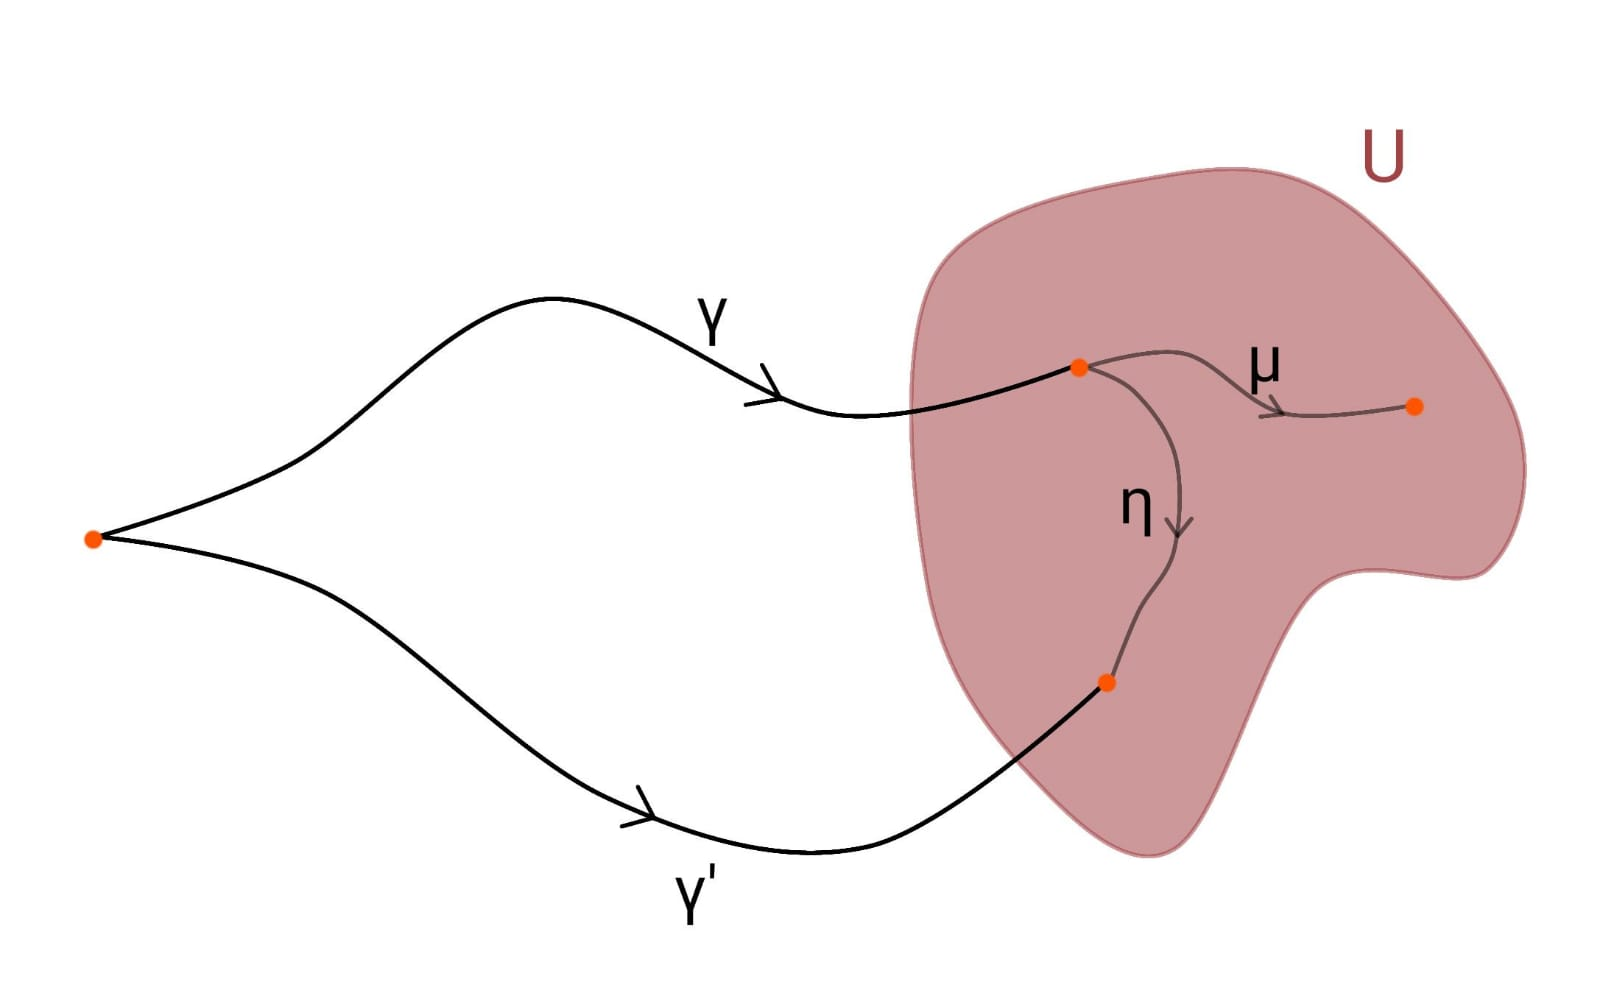
\includegraphics[width=0.8\linewidth]{conteudo/fig-cobertura-P(X,x_0).jpeg}
         \caption{Verificação de quando dois abertos $U_{[\gamma]}$ são iguais}
         \label{fig:cobertura-P(X,x_0)}
     \end{figure} 

     
     Verifiquemos que abertos desta forma constituem uma base para $P(X,x_0)$ e, além disso, que $q:U_{[\gamma]}\rightarrow U$ é um homeomorfismo, o que nos aproxima da verificação de que $q:P(X,x_0)\rightarrow X$ é um espaço de recobrimento.\newline

     De fato, temos as seguintes informações:

     \begin{enumerate}
        \item  $q:U_{[\gamma]}\rightarrow U$ é mapa injetor.\newline
        
        Escolhas diferentes de $\eta$ em $U$ que ligam $\gamma(1)$ a um mesmo ponto $x\in U$, isto é, dois caminhos $\eta_1$ e $\eta_2$ nessas condições tais que $q([\gamma*\eta_1])=q([\gamma*\eta_2])$, são tais que $\eta_1\sim \eta_2 (\text{rel }\partial I)$. Isso ocorre porque $i^*:\pi_1(U,x)\rightarrow \pi_1(X,x)$ é trivial, o que leva a conclusão de que dada a curva fechada $\eta_1* \overline{\eta_2}$ com ponto base $x$, temos a igualdade $[\eta_1* \overline{\eta_2}]=[c_x]\in \pi_1(X,x)$ e, portanto, $$\eta_1\sim\eta_1*(\overline{\eta_2}*\eta^2)\sim (\eta_1*\overline{\eta_2})*\eta^2\sim c_x*\eta_2\sim  \eta_2~(\text{rel }\partial I).$$  Dessa forma, $\gamma*\eta_1\sim \gamma*\eta_2 (\text{rel }\partial I)$ e, portanto, $[\gamma*\eta_1]=[\gamma*\eta_2]$. A situação é descrita na figura \ref{fig:restricao-de-q-é-injetor}.

        \begin{figure}[h!]
         \centering
         \includegraphics[width=0.8\linewidth]{conteudo/fig-restricao-de-q-é-injetor.jpeg}
         \caption{Restrição de $q$ a $U_{[\gamma]}$ é mapa injetor}
         \label{fig:restricao-de-q-é-injetor}
     \end{figure} 
     
         \item $q:U_{[\gamma]}\rightarrow U$ é mapa sobrejetor.\newline
         
         Como $U$ é conexo por caminhos, sempre é possível encontrar curva $\eta$ em $U$ que ligue $\gamma(1)$ a qualquer outro ponto de $U$.\newline
         
         \item $\tilde{\mathcal{B}}=\{U_{[\gamma]}|~U\in \mathcal{B}, \gamma:I\rightarrow X\text{ com }\gamma(0)=x_0\text{ e }\gamma(1)=x\in U\}$ é base para a topologia de $P(X,x_0)$.\newline
         
        Os abertos de $\tilde{\mathcal{B}}$ realmente cobrem $P(X,x_0)$ porque dado qualquer $[\gamma]\in P(X,x_0)$, se $\gamma(1)=x$, então existe $U\in \mathcal{B}$ vizinhança de $x$ de forma que $[\gamma]\in U_{[\gamma]}$.
        Além disso, dados $U_{[\gamma_1]} $ e $V_{\gamma_2}$ quaisquer em $\tilde{\mathcal{B}}$ e um elemento $[\gamma]\in U_{\gamma_1}\cap V_{\gamma_2}$, temos que $U_{[\gamma]}= U_{[\gamma_1]}$ e $V_{[\gamma]}=V_{[\gamma_2]}$, pois mostramos anteriormente que em geral $U_{[\gamma]}=U_{[\gamma']}$ se e somente se $[\gamma']\in U_{[\gamma]}$. Assim, $\gamma(1)\in U$, $\gamma(1)\in V$ e é possível tomar $W\in \mathcal{B}$ tal que $W\subset U\cap V$ é vizinhança de $\gamma(1)$, uma vez que $\mathcal{B}$ é base. Dessa forma, $W_{[\gamma]}\subset U_{[\gamma]}\cap V_{[\gamma]}=U_{[\gamma_1]}\cap V_{[\gamma_2]}$ pertence a $\tilde{\mathcal{B}}$ e contém $[\gamma]=[\gamma*c_{\gamma(1)}]$\newline
         

         \item $q:U_{[\gamma]}\rightarrow U$ é de fato homeomorfismo.\newline
         
            Seja $V\subset U$ aberto em $\mathcal{B}$. A pré-imagem desse aberto pela restrição de $q$ em $U_[\gamma]$ é $q^{-1}(V)\cap U_{[\gamma]}= V_{[\gamma']}$ para qualquer $[\gamma']\in U_{[\gamma]}$ tal que $\gamma'(1)\in V$, uma vez que $V_{[\gamma']} \subset U_{[\gamma']}=U_{[\gamma]}$ e já vimos que $q:V_{[\gamma']}\rightarrow V$ é uma bijeção. 
            
            De fato, se $V'\subset U$ é aberto qualquer, $V'=\underset{\lambda\in \Lambda, U_\lambda\in \mathcal{B}}{\bigcup} U_\lambda$ união enumerável de abertos e a pré imagem de $V'$ pela restrição de $q$ em $U_{[\gamma]}$ é $$q^{-1}(V')\cap U_{[\gamma]} =\underset{\lambda\in \Lambda, U_\lambda\in \mathcal{B}}{\bigcup} q^{-1}(U_\lambda)\cap U_{[\gamma]} = \underset{\lambda\in \Lambda, U_\lambda\in \mathcal{B}}{\bigcup} (U_\lambda)_{[\gamma_\lambda]}$$ para qualquer $[\gamma_\lambda]\in U_{[\gamma]}$ tal que $\gamma_\lambda(1)\in U_\lambda$. De fato, a pré-imagem é união enumerável de abertos e, portanto, aberta.
            
            
            Além disso, como $q(V_{[\gamma]})=V$ aberto e $\tilde{\mathcal{U}}$ é base, temos que dado qualquer aberto $V''\subset U_{[\gamma]}$ é $V''=\underset{\lambda \in \Lambda, U_\lambda \in \tilde{\mathcal{U}}}{\bigcup} U_\lambda$ união enumerável de abertos e então $q(V'')=\underset{\lambda \in \Lambda, U_\lambda \in \tilde{\mathcal{U}}}{\bigcup} q(U_\lambda)$, onde $q(U_\lambda)\in \mathcal{B}$ para todo $\lambda \in \Lambda$. Isto é, $q(V'')$ é união enumerável de abertos e, portanto, aberto.\newline

        \item $q:P(X,x_0)\rightarrow X$ é contínuo.\newline
        
            Para todo aberto $V\subset X$, temos que $V=\underset{\lambda\in \Lambda, V_\lambda \in \mathcal{B}}{\bigcup} V_\lambda$ para certos abertos $V_\lambda$ em $\mathcal{B}$.

            Temos que $$q^{-1}(V)=q^{-1}(\underset{\lambda\in \Lambda, V_\lambda \in \mathcal{B}}{\bigcup} V_\lambda)=\underset{\lambda\in \Lambda, V_\lambda \in \mathcal{B}}{\bigcup}q^{-1}(V_\lambda),$$ onde $q^{-1}(V_\lambda)=\underset{\gamma, (V_\lambda)_[\gamma] \in \tilde{\mathcal{B}}}{\bigcup} (V_\lambda)_{[\gamma]}$.

            Assim, todo $[\gamma]\in q^{-1}(V)$ é tal que $\gamma(1)\in V$ e, portanto, $\gamma(1)\in V_{\lambda_0}$ para algum $\lambda_0\in \Lambda$. Isto significa que $[\gamma]\in (V_{\lambda_0})_\gamma\subset q^{-1}(V)$ aberto. Portanto, $q^{-1}(V)$ é de fato aberto, como queríamos.\newline\newline
     \end{enumerate}


    Assim, temos que para todo $x\in X$ existe $U\in \mathcal{B}$ vizinhança de $x$ tal que  $p^{-1}(U)=\underset{[\gamma]}{\sqcup} U_{[\gamma]}$, onde cada $U_{[\gamma]}$ é homeomorfo a $U$. Essa união é disjunta pois se $U_{[\gamma_1]}\neq U_{[\gamma_2]}$ e $[\gamma]\in U_{[\gamma_1]}\cap U_{[\gamma_2]}$, então $U_{[\gamma]}=U_{[\gamma_1]}$ e $U_{[\gamma]}=U_{[\gamma_2]}$, o que implica $U_{[\gamma_1]}=U_{[\gamma_2]}$, uma contradição. Portanto, $U$ é aberto uniformemente recoberto de $X$ e isso conclui a nossa demonstração de que $P(X,x_0)$ é espaço de recobrimento.\newline

    Resta, por último, verificar que $P(X,x_0)$ é 1-conexo:

    \begin{enumerate}
        \item $P(X,x_0)$ é conexo por caminhos.\newline
        
            De fato, para todo $[\gamma]\in P(X,x_0)$, tome $\gamma_t:[0,1]\rightarrow X$ como a curva definida por 

            $$\begin{cases}
                \gamma(s), \text{ se }s\in [0,t]\\
                \gamma(t), \text{ se }s\in [t,1]
            \end{cases}$$

            Assim a curva $t\mapsto [\gamma_t]$ é um caminho em $P(X,x_0)$ que começa em $[c_{\gamma(0)}]=[c_{x_0}]$, curva constante em $\gamma(0)=x_0$, e termina em $[\gamma]$.

            Como isso vale para todo $[\gamma]$ em $P(X, x_0)$, então esse espaço é conexo por caminhos.\newline
        
        \item $\pi_1(P(X,x_0), [c_{x_0}])=0$\newline
        
            Para esta verificação mostraremos que $p_*: \pi_1(P(X,x_0), [c_{x_0}])\rightarrow \pi_1(X,x_0)$ é trivial.\newline

            Um elemento na imagem de $p_*$ é da forma $[\gamma]$ onde $\gamma$ é curva fechada com ponto base $x_0$ e seu levantamento também deve ser curva fechada, neste caso com ponto base $[c_{x_0}]$. Foi visto no item anterior que $t\mapsto [\gamma_t]$ levanta $\gamma$, começando em $[x_0]$ e terminando em $[\gamma_1]=[\gamma]$. Se esse levantamento é uma curva fechada, então $[\gamma]=[c_{x_0}]$ e o mapa de fato é trivial.

            Como $p_*$ é injetivo segundo o lema \ref{homomorfismo-induzido-por-recobrimento-prop}, então o fato de ser trivial implica $\pi_1(P(X,x_0), [c_{x_0}])=0$, como queríamos.\newline
        
    \end{enumerate}

    Assim, verificamos que $q: P(X,x_0)\rightarrow X$ é de fato um recobrimento 1-conexo e concluí-se por fim que, nas condições do enunciado, quando $X$ é semi-localmente simplesmente conexo, $X$ admite recobrimento 1-conexo.
    
\end{dem}

\begin{titlemize}{Lista de consequências}
	\item \hyperref[pertence-a-base-se-e-somente-se-possui-i-trivial]{Proposição - nova descrição da base $\mathcal{B}$};\\ %'consequencia1' é o label onde o conceito Consequência 1 aparece
    %\item \hyperref[espaço-1-conexo-def]{Espaço 1-conexo}
    \item \hyperref[recobrimento-universal]{Recobrimento universal}
\end{titlemize}

%---------------------------------------------------------------------------------------------------------------------!Draft!-----------------------------------------------------------------------------------------------------------------
\subsection{Descrição de $\tilde{\mathcal{B}}$ em termos de $X$} %afirmação aqui significa teorema/proposição/colorário/lema
\label{descrição-da-base-do-recobrimento-prop}
\begin{titlemize}{Lista de dependências}
	\item \hyperref[espaco-de-recobrimento-def]{Espaço de recobrimento};\\ %'dependencia1' é o label onde o conceito Dependência 1 aparece (--à arrumar um padrão para referencias e labels--) 
	\item \hyperref[espaço-1-conexo-def]{Espaço 1-conexo};\\
% quantas dependências forem necessárias.
\end{titlemize}


%Comentário sobre os objetos envolvidos na afirmação.



\begin{af}[Base para recobrimento 1-conexo]% ou af(afirmação)/prop(proposição)/corol(corolário)/lemma(lema)/outros ambientes devem ser definidos no preambulo de Alg.Top-Wiki.tex 
	Seja $p: E\rightarrow X$ um recobrimento com $X $ localmente conexo por caminhos e $E$ 1-conexo. A base $\tilde{\mathcal{B}}$ da topologia de $E$ definida em \ref{base-para-topologias-em-recobrimento-prop} pode ser descrita em termos de $X$ em dois casos:\newline

    \textbf{Caso 1:} Seja $U\in \mathcal{B}$ um aberto uniformemente recoberto com $x_0\in U$.\newline

    Em um espaço $\tilde{U}$ que seja placa de $U$ é possível levantar um caminho $\eta$ entre $x_0$ e $y_0$, em que $y_0\in U$ qualquer já que o espaço é conexo por caminhos, para um caminho $\tilde{\eta}$ entre $\tilde{x_0}$ e $\tilde{y_0}$ onde estes são pontos tais que $p(\tilde{x_0})=x_0$ e $p(\tilde{y_0})=y_0$.\newline

    Defina $U_{\tilde{x_0}}=\{\tilde{\eta}_{\tilde{x_0}}(1)|~\eta:I\rightarrow U\text{ e }\eta(0)=x_0\}$. A partir desta definição, é possível dizer que todas as placas de $U$ podem ser escritas como $U_{\tilde{x_0}}$ para algum $\tilde{x_0}$, que é o único valor existente na placa tal que $p(\tilde{x_0})=x_0$. Isto é,

    $$p^{-1}(U)=\underset{\tilde{x_0}\in p^{-1}(x_0)}{\sqcup} U_{\tilde{x_0}}$$
    


    \textbf{Caso 2:} Seja $U\subset X$ aberto conexo por caminhos e uniformemente recoberto, isto é, $U\in \mathcal{B}$. Tome $x\in U$ e seja $\tilde{x}\in E$ tal que $p(\tilde{x})=x$.\newline
    
    Fixe uma curva $\gamma: I\rightarrow X$ com $\gamma(0)=x_0$ e $\gamma(1)=x$, isto é, $[\gamma]\in q^{-1}(x)$. Note que $q$ é a função $q:P(X,x_0)\rightarrow X$ onde $P(X,x_0)=\{[\gamma]|~\gamma(0)=x_0\}$ definida por $q([\gamma])=\gamma(1)$.\newline
    
    Pode-se escrever $U$ como o espaço formado por $\gamma*\eta(1)$ para algum $\eta:I\rightarrow U$ tal que $\eta(0)=x$. Isto é, é possível descrever o aberto de $\tilde{\mathcal{B}}$ que é placa de $p$ sobre $U$ e vizinhança de $\tilde{x}$ como $$\tilde{U}_{\tilde{x}}=\{(\widetilde{\gamma*\eta})_{e_0}(1)|~\eta:I\rightarrow U,~\eta(0)=x\},$$ onde $e_0$ é tal que $\tilde{\gamma}_{e_0}(1)=\tilde{x}$.
    
    
    
	
\end{af}



\begin{titlemize}{Lista de consequências}
	\item \hyperref[pertence-a-base-se-e-somente-se-possui-i-trivial]{Proposição - nova descrição da base $\mathcal{B}$};\\ %'consequencia1' é o label onde o conceito Consequência 1 aparece
%	\item \hyperref[]{}
\end{titlemize}

%[Bianca]: Um arquivo tex pode ter mais de uma afirmação (ou definição, ou exemplo), mas nesse caso cada afirmação deve ter seu próprio label. Dar preferência para agrupar afirmações que dependam entre sí de maneira próxima (um teorema e seu corolário, por exemplo)
%---------------------------------------------------------------------------------------------------------------------!Draft!-----------------------------------------------------------------------------------------------------------------
\subsection{Base da topologia de $X$ possui $i^*$ trivial para todos os elementos quando há recobrimento 1-conexo} %afirmação aqui significa teorema/proposição/colorário/lema
\label{pertence-a-base-se-e-somente-se-possui-i-trivial}
\begin{titlemize}{Lista de dependências}
	\item \hyperref[base-para-topologias-em-recobrimento-prop]{Base para as topologias em um recobrimento};\\ %'dependencia1' é o label onde o conceito Dependência 1 aparece (--à arrumar um padrão para referencias e labels--) 
	\item \hyperref[recobrimento-1-conexo-prop]{Existe recobrimento 1-conexo se e somente se X slsc};\\
    \item \hyperref[descrição-da-base-do-recobrimento-prop]{Descrição de $\tilde{\mathcal{B}}$ em termos de $X$};\\
    \item \hyperref[1-conexo-prop]{Propriedades de 1-conexo};\\
    \item \hyperref[levantamento-de-homotopia-prop]{Levantamento de Homotopia}
% quantas dependências forem necessárias.
\end{titlemize}
%Comentário sobre os objetos envolvidos na afirmação.
\begin{prop}% ou af(afirmação)/prop(proposição)/corol(corolário)/lemma(lema)/outros ambientes devem ser definidos no preambulo de Alg.Top-Wiki.tex 
	Sejam $p:E\rightarrow X$ um recobrimento 1-conexo e $U\subset X$ um aberto conexo por caminhos. Então $U\in \mathcal{B}$, onde $\mathcal{B}$ é base para a topologia de $E$ conforme definida em \ref{base-para-topologias-em-recobrimento-prop}, se se somente se $i_*:\pi_1(U,x)\rightarrow \pi_1(X,x)$ é trivial.\\

\end{prop}
\begin{dem}
    Por um lado, se $U\in \mathcal{B}$ temos que, dada a inclusão $i:U\rightarrow X$, $i_*:\pi(U,x)\rightarrow \pi(X,x)$ é um mapa trivial segundo argumentação realizada no início da demonstração do Teorema \ref{recobrimento-1-conexo-prop}.\newline

    Por outro lado, se $i_*:\pi_1(U,x)\rightarrow \pi_1(X,x)$ é trivial, vamos verificar que $U$ é uniformemente recoberto. Em particular, verifiquemos que $p^{-1}(U)=\underset{[\gamma]\in q^{-1}(X)}{\bigsqcup} \tilde{U}_{[\gamma]}$ onde $$\tilde{U}_{[\gamma]}=\{(\widetilde{\gamma*\eta})_{\tilde{x}}(1)|~\eta:I\rightarrow U,~\eta(0)=x\}$$, da mesma forma que é descrito no "caso 2" da Afirmação \ref{descrição-da-base-do-recobrimento-prop}. Isto é, $\tilde{U}_{[\gamma]}\in \tilde{B}$.

    Para tal, verifiquemos:

    \begin{enumerate}
        \item $\tilde{U}_{[\gamma]}\subset p^{-1}(U)$ para todo $[\gamma]$ pois
        $$p(\tilde{U}_{[\gamma]})=\{p((\widetilde{\gamma*\eta})_{\tilde{x}}(1))|~\eta:I\rightarrow U,~\eta(0)=x\}=$$$$=\{(\gamma*\eta)(1)|~\eta:I\rightarrow U,~\eta(0)=x\}=\{\eta(1)\in U|~\eta:I\rightarrow U,~\eta(0)=x\}\subset U$$\newline

        \item $p^{-1}(U)\subset \underset{[\gamma]\in q^{-1}(x)}{\bigcup} \tilde{U}_{[\gamma]}$

        Seja $\tilde{y}\in p^{-1}(U)$, seja $\eta:I\rightarrow U$ com $\eta(0)=x$ e $\eta(1)=y=p(\tilde{y})$ e seja $\tilde{x}=\tilde{\overline{\eta}}_{\tilde{y}}(1)$, de forma que $p(\tilde{x})=x$.

        Seja $ \xi:I\rightarrow E$ com $\xi(0)=e_0$, $\xi(1)=\tilde{x}$ e seja $\gamma=p\circ \xi$. Então $ \tilde{y}\in \tilde{U}_{[\gamma]}$ pois $(\widetilde{\gamma * \eta})_{e_0}(1)=\tilde{\eta}_{\tilde{x}}(1)=\tilde{y}$.\newline

        \item Se $[\gamma_0]\neq [\gamma_1]\in q^{-1}(x)$, então $ \tilde{U}_{[\gamma_0]}\cap \tilde{U}_{[\gamma_1]}=\emptyset$

        Suponha que $\tilde{y}\in \tilde{U}_{[\gamma_0]}\cap\tilde{U}_{[\gamma_1]}$. Sejam $\eta_0, \eta_1: I\rightarrow U$ curvas tais que $(\widetilde{\gamma_0*\eta_0})_{e_0}(1)=(\widetilde{\gamma_1*\eta_1})_{e_0}(1)=\tilde{y}$, como representado na figura \ref{fig:classes-distintas-de-curvas} a seguir.

\begin{figure}[h!]
         \centering
         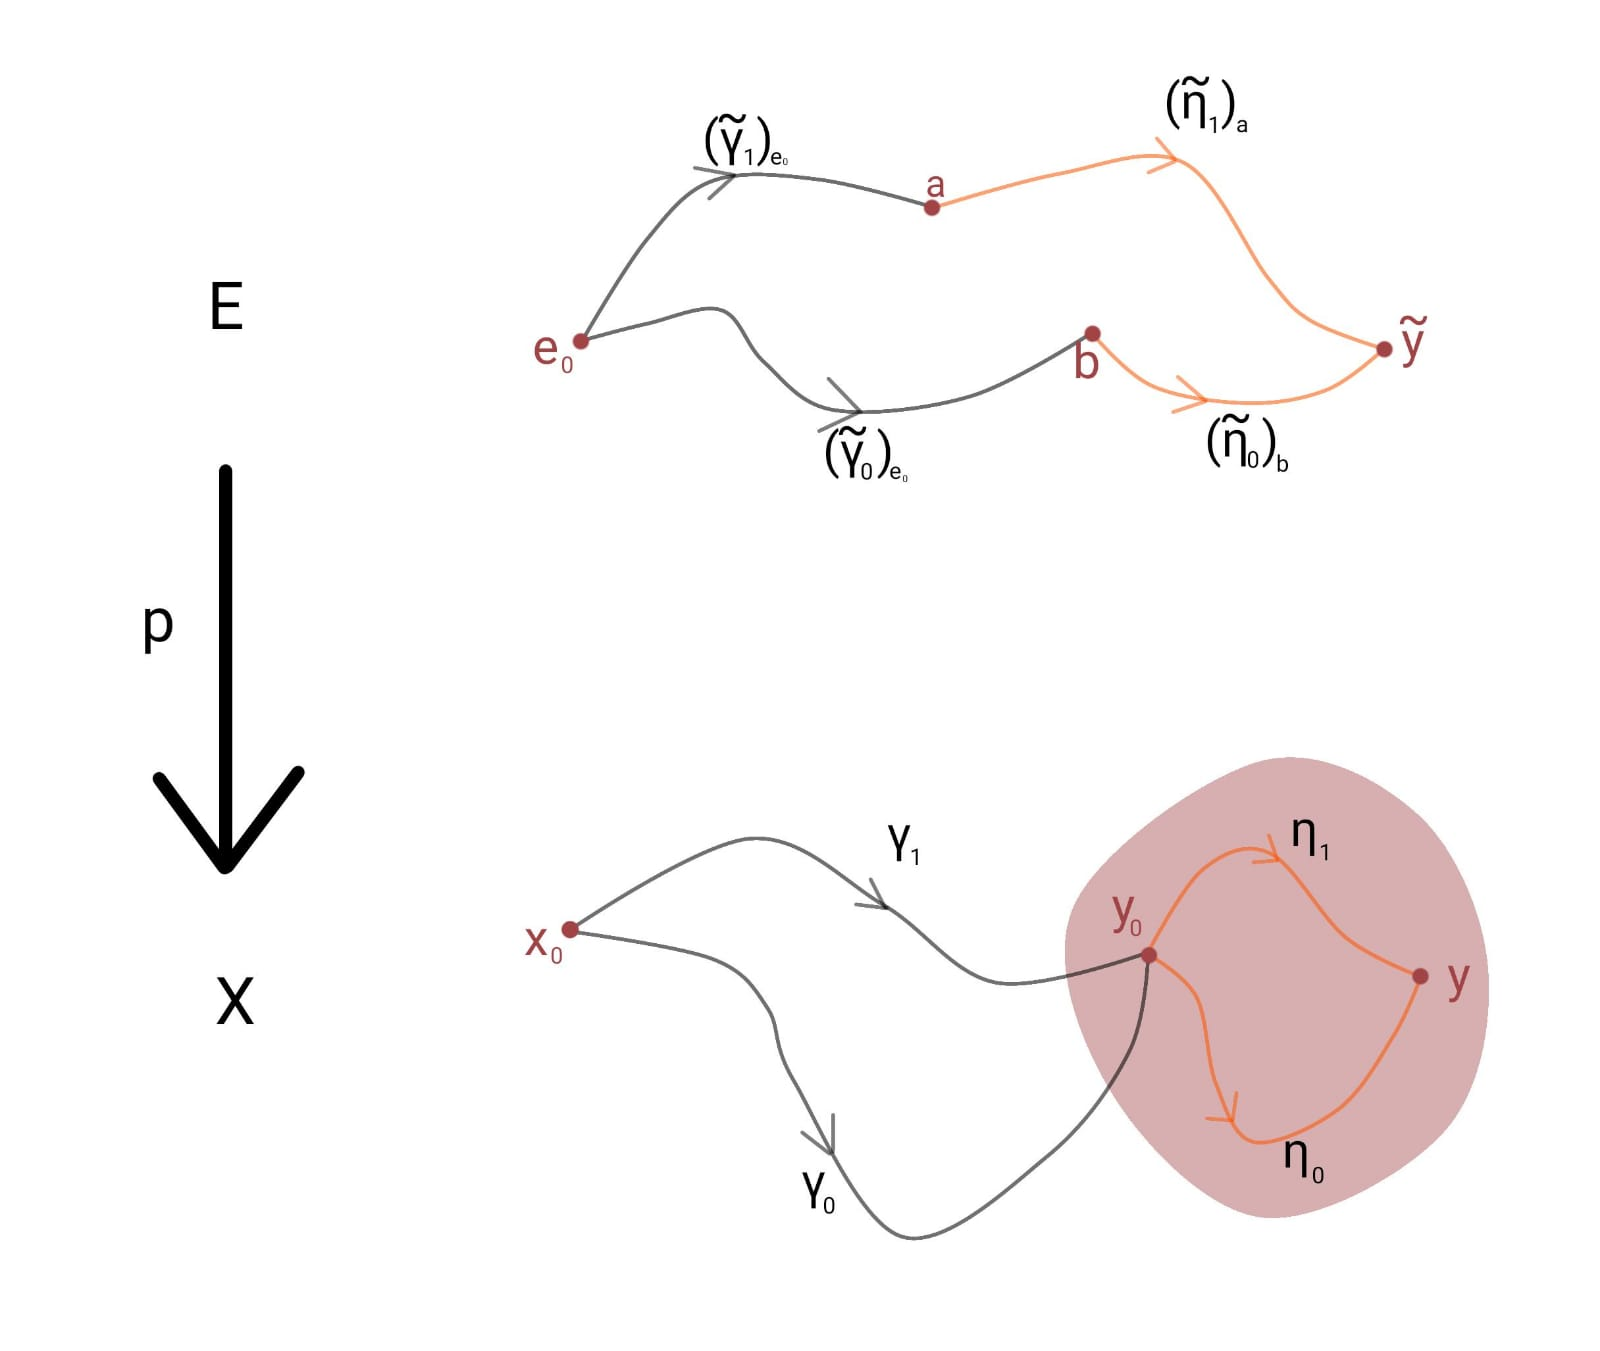
\includegraphics[width=0.8\linewidth]{conteudo/fig-classes-distintas-de-curvas.jpeg}
         \caption{Classes distintas de curvas, mas $\tilde{y}$ na intersecção dos abertos}
         \label{fig:classes-distintas-de-curvas}
     \end{figure} 

        
        Assim, temos que $p\circ(\widetilde{\gamma_0*\eta_0})_{e_0}(1)=y=p\circ(\widetilde{\gamma_1*\eta_1})_{e_0}(1)$ e portanto $\eta_0(1)=y=\eta_1(1)$.

        Na mesma figura, é possível notar que $\eta_0*\overline{\eta}_1$ é um laço em $U$ com ponto base $y$. Como nos foi dado que $i^*:\pi(U,x)\rightarrow \pi_1(X,x)$ é trivial e $U$ conexo por caminhos, temos que

        $$(\eta_0*\overline{\eta}_1)\sim c_y~(\text{rel}~\partial I) \Rightarrow (\widetilde{\eta_0 * \overline{\eta_1}})_{\tilde{y}}\sim  c_{\tilde{y}}~(\text{rel}~\partial I)\Rightarrow (\tilde{\gamma}_0)_{e_0}(1)=(\tilde{\gamma}_1)_{e_0}(1),$$ diferentemente do que a imagem indica.

        Como $E$ é 1-conexo, utilizando a Proposição \ref{1-conexo-prop} concluí-se que $[\gamma_0]=[\gamma_1]$, um absurdo por contradizer a hipótese inicial.\newline
        

    
        \item A restrição $p|_{\tilde{U}_{[\gamma]}}:\tilde{U}_{[\gamma]}\rightarrow U $ é bijeção

        Para verificar a sobrejetividade basta notar que para todo $y\in U$ é possível tomar a curva $\eta:I\rightarrow U$ tal que $\eta(0)=x$ e $\eta(1)=y$. Temos que se $\tilde{y}=(\widetilde{\gamma*\eta})_{e_0}(1)\in \tilde{U}_{[\gamma]}$, então $p(\tilde{y})=y$, como queríamos.

        Para a verificação da injetividade, basta supor que $p((\widetilde{\gamma*\eta_0})_{e_0}(1))=p((\widetilde{\gamma*\eta_1})_{e_0}(1))$ onde $\eta_0, \eta_1:I\rightarrow U$ são tais que $\eta_0(0)=x=\eta_1(0)$ e $\eta_0(1)=\eta_1(1)$. Portanto, $\eta_0*\overline{\eta}_1$ é laço e assim $\eta_0\sim \eta_1~(\text{rel }\partial I)$.
        Isso significa que, se $\tilde{x}=\tilde{\gamma}_{e_0}(1)$, então $(\tilde{\eta}_0)_{\tilde{x}}(1)= (\tilde{\eta}_1)_{\tilde{x}}(1)$ segundo Corolário presente em \ref{levantamento-de-homotopia-prop}. Assim, $(\widetilde{\gamma*\eta_0})_{e_0}(1)=(\gamma*\eta_1)_{e_0}(1)$.\newline

        \item A restrição $p|_{\tilde{U}_{[\gamma]}}$ é aplicação aberta pois $\tilde{U}_{[\gamma]}\in \tilde{\mathcal{B}}$ é uma placa do recobrimento.\newline
    \end{enumerate}

    Assim, verificamos que $U$ é uniformemente recoberto, isto é, $U \in \mathcal{B}$ como queríamos.\newline
\end{dem}

O resultado acima implica que a base $\mathcal{B}$ pode ser descrita como $\mathcal{B}=\{U\subset X|~U\text{ é conexo por caminhos e }i_*:\pi_1(U,x)\rightarrow \pi_1(X,x)\text{ é trivial}\}$

%\begin{titlemize}{Lista de consequências}
%	\item \hyperref[consequencia1]{Consequência 1};\\ %'consequencia1' é o label onde o conceito Consequência 1 aparece
%	\item \hyperref[]{}
%\end{titlemize}

%[Bianca]: Um arquivo tex pode ter mais de uma afirmação (ou definição, ou exemplo), mas nesse caso cada afirmação deve ter seu próprio label. Dar preferência para agrupar afirmações que dependam entre sí de maneira próxima (um teorema e seu corolário, por exemplo)


%%% Local Variables:
%%% mode: LaTeX
%%% TeX-master: "../Alg.Top-Wiki"
%%% End:

%-------------------------------------------------------------------------------------------------------------!Draft!-------------------------------------------------------------------------------------------------------------------------
\section{Ações de grupos e recobrimentos}
\label{ações-de-grupos-e-recobrimentos}

\begin{titlemize}{Lista de Dependências}
	\item \hyperref[homotopia]{Homotopia}; %assunto1 é o label onde o Assunto 1 aparece
	\item \hyperref[espaco-de-recobrimento]{Espaços de recobrimentos};
    \item\hyperref[grupo-fundamental]{Grupo Fundamental}
\end{titlemize}

Dedicamos essa seção para estudar a relação entre ações de grupos, recobrimentos e grupos fundamentais. 

%---------------------------------------------------------------------------------------------------------------------!Draft!-----------------------------------------------------------------------------------------------------------------
\subsection{Ações de grupo}
\label{ações-de-grupo-def}

%\begin{titlemize}{Lista de dependências}
	%\item \hyperref[dependecia1]{Dependência 1};\\ %'dependencia1' é o label onde o conceito Dependência 1 aparece (--à arrumar um padrão para referencias e labels--) 
	%\item \hyperref[]{};\\
% quantas dependências forem necessárias.
%\end{titlemize}

\begin{defi}[Ação de Grupo]
	Seja $G$ um grupo com elemento neutro 1 e $X$ um conjunto. Uma ação do grupo $G$ sobre o conjunto $X$ pela esquerda é uma função
 \[\psi: G\times X \longrightarrow X\] satisfazendo:
 
 \begin{itemize}
     \item[(i)] $\psi(1,x) = x \  \forall\  x \in X$
     \item[(ii)] $\psi(g,\psi(h,x)) = \psi(gh,x) \ \forall\ x \in X,\ \forall\ g,h \in G$
 \end{itemize}
 Neste caso, dizemos que $G$ age pela esquerda em $X$.\\
 
\noindent Analogamente,\\
 Uma ação do grupo $G$ sobre o conjunto $X$ pela direita é uma função\\
 $\psi: X\times G \longrightarrow X$ satisfazendo:
 
 \begin{itemize}
     \item[(i)] $\psi(x,1) = x ,\  \forall\  x \in X$
     \item[(ii)] $\psi(\psi(x,g), h) = \psi(x,gh), \ \forall\ x \in X,\ \forall\ g,h \in G$
 \end{itemize}
 Neste caso, dizemos que $G$ age pela direita em $X$.

\end{defi}

Outras notações: $\psi(g,x) = \psi_{g}(x)$ ou simplesmente $g\cdot x$ se a ação (à esquerda) estiver explícita no contexto.\\
Além disso, escrevemos $G\circlearrowright X$ para denotar que $G$ age em $X$.


\begin{titlemize}{Lista de consequências}
	\item \hyperref[ações-de-grupo-propriamente-descontínuas-def]{Definição de ação de grupo propriamente descontínua}; %'consequencia1' é o label onde o conceito Consequência 1 aparece
\end{titlemize}

%[Bianca]: é mais fácil criar a lista de dependências do que a de consequências.

\input{conteudo/açoes-de-grupos-ex}
%---------------------------------------------------------------------------------------------------------------------!Draft!-----------------------------------------------------------------------------------------------------------------
\subsection{Ações de Grupos Propriamente descontínuas}
\label{ações-de-grupo-propriamente-descontínuas-def}
\begin{titlemize}{Lista de dependências}
	\item \hyperref[ações-de-grupo-def]{Ações de grupos};\\ %'dependencia1' é o label onde o conceito Dependência 1 aparece (--à arrumar um padrão para referencias e labels--) 
% quantas dependências forem necessárias.
\end{titlemize}
\begin{defi}[Ação propriamente descontínua]
	Dizemos que a ação:
	\begin{align*}
    		\psi_{g}: G\times X &\longrightarrow X\\
    		\psi_{g}(x) &\longmapsto gx
	\end{align*}

\noindent é própriamente descontínua se $\forall x \in X$, existe um aberto $U \subset X$ de $x$ tal que:
\[gU \cap U \neq \emptyset \  \Rightarrow g = 1\]

\noindent onde $gU = \{gy\  |\  y \in U\} = \psi_{g}(U) \subset U$ e
\begin{align*}
    \psi_{g}: X&\longrightarrow X\\
    \psi_{g}(y)&\longmapsto gy
\end{align*}
Uma possível intuição geométrica para uma ação propriamente descontínua, é interpretá-la como uma função $\psi$ que leva os pontos $x$ do espaço para "longe" de sua posição inicial.
\end{defi}
\begin{titlemize}{Lista de consequências}
	\item \hyperref[ações-de-grupos-e-recobrimentos-prop]{Ações de grupos propriamente descontínuas geram recobrimento}; %'consequencia1' é o label onde o conceito Consequência 1 aparece
    \item \hyperref[ações-de-grupos-e-gr-fundamental-prop]{Ações de grupo e grupos fundamentais}
\end{titlemize}

%[Bianca]: é mais fácil criar a lista de dependências do que a de consequências.

%-------------------------------------------------------------------------------------------------------------!Draft!-------------------------------------------------------------------------------------------------------------------------
\subsection{Ações de Grupos e Recobrimentos}
\label{ações-de-grupos-e-recobrimentos-prop}

\begin{titlemize}{Lista de Dependências}
	\item \hyperref[ações-de-grupo-def]{Ações de Grupos}; %'dependencia1' é o label onde o conceito Dependência 1 aparece (--à arrumar um padrão para referencias e labels--) 
    \item \hyperref[ações-de-grupo-propriamente-descontínuas-def]{Ações de grupos propriamente descontínuas}% quantas dependências forem necessárias.
 
\end{titlemize}

Uma pergunta natural que surge ao longo do estudo de topologia algébrica é:
Para quais ações  G $\circlearrowright X$ temos que a aplicação quociente $p: X \rightarrow\mkern-18mu \quad{^{\textstyle X}\big/_{\textstyle G}}$ é um recobrimento?\\\\
onde $\quad{^{\textstyle X}\big/_{\textstyle G}} =\mkern-18mu \quad{^{\textstyle X}\big/_{\textstyle \sim}}$, definindo $\sim$ como a seguinte relação de equivalência: \[x\sim y \Leftrightarrow \exists \ g \in G \mid y = gx\]
\\
Assim, obtemos a seguinte proposição:\\

\begin{thm}[Ações propriamente descontínuas geram recobrimentos]% ou af(afirmação)/prop(proposição)/corol(corolário)/lemma(lema)/outros ambientes devem ser definidos no preambulo de Alg.Top-Wiki.tex 
	Seja \\ $\Psi:G \times X \longrightarrow X$ uma ação propriamente descontínua. Então a aplicação quociente
 $p: X \longrightarrow\mkern-18mu \quad{^{\textstyle X}\big/_{\textstyle G}}$ é um recobrimento.
\end{thm}

\begin{dem}
    Vamos mostrar que dado $[x] \in\mkern-18mu \quad{^{\textstyle X}\big/_{\textstyle G}}$, existe $U \subset\mkern-18mu \quad{^{\textstyle X}\big/_{\textstyle G}}$ \\
    vizinhança uniformemente recoberta de $[x]$:\\\\
    Note que \[p^{-1}(U) = \coprod_{g \in G} V_g \] onde $V_g \subset X $ são abertos e ainda:
    \[p\restriction_{V_g}:V_g \rightarrow U\] é uma relação de equivalência.\\
    Dado $x \in X$, seja $V_1$ vizinhança de $x$ tal que $gV_1\cap V_1 \neq \emptyset \Rightarrow g = 1$\\
    Sejam agora $V_g = gV_1$ e $U = p(V_1)$, vizinhança de $[x]$\\
    Então temos:\\
    $$
        \begin{cases}
            p^{-1}(U) = \coprod_{g\in G} V_g\\
            p\restriction_{V_1}:V_1 \rightarrow U \text{ é homeomorfismo}
        \end{cases}
    $$\\
    Falta mostrar que $p\restriction_{V_g}$ é um homeomorfismo. Mas temos que:

    \[
        p\restriction_{V_g} = p\restriction_{V_1} \circ \Psi_{g^{-1}}
    \]
    É composição de homeomorfismos
\end{dem}

\begin{titlemize}{Lista de consequências}
	%'consequencia1' é o label onde o conceito Consequência 1 aparece
    \item \hyperref[ações-de-grupos-e-gr-fundamental-prop]{Encontrando o grupo fundamental através de uma ação propriamente descontínua}
\end{titlemize}
%[Bianca]: Decidir o que é um assunto e o que é apenas um resultado/definição pode ser uma tarefa não trivial. A princípio essa tarefa será realizada pelos alunos, em conjunto. Se for necessário podem entrar em contato com o professor Ivan ou comigo. 


% Cada novo assunto deve ser adcionado no corpo do texto, como explicado no arquivo Alg.Top-Wiki.tex.

%---------------------------------------------------------------------------------------------------------------------!Draft!-----------------------------------------------------------------------------------------------------------------
\subsection{Ação propriamente descontínua e grupo fundamental} %afirmação aqui significa teorema/proposição/colorário/lema
\label{ações-de-grupos-e-gr-fundamental-prop}
\begin{titlemize}{Lista de dependências}
	\item \hyperref[ações-de-grupo-propriamente-descontínuas-def]{Ações de grupos propriamente descontínuas}; %'dependencia1' é o label onde o conceito Dependência 1 aparece (--à arrumar um padrão para referencias e labels--) 
	\item \hyperref[grupo-fundamental-def]{Grupo fundamental};\\
% quantas dependências forem necessárias.
\end{titlemize}
Nesse teorema vamos encontrar uma relação entre ações propriamente descontínuas e grupos fundamentais.

\begin{thm}[Ação propriamente descontínua e grupo fundamental]% ou af(afirmação)/prop(proposição)/corol(corolário)/lemma(lema)/outros ambientes devem ser definidos no preambulo de Alg.Top-Wiki.tex 
	Suponha que $X$ é 1-conexo e que $B = \mkern-18mu\quad{^{\textstyle X}\big/_{\textstyle G}}$, tal que $G\circlearrowright X$ é uma ação propriamente descontínua, então:\\
    \[\pi_1(B,b_0)\cong G\]
	\begin{dem}
        Seja $b=[x]$ e defina:\\
        \[\Phi_x:\pi_1(B,b)\longrightarrow G\]\\
        tal que:
        \[\Phi_x([\alpha]) = g \iff \widetilde{\alpha}_x(1)=gx\]\\
    Defina agora, $\varphi_x:\pi_1(B,b)\longrightarrow p^{-1}(b)$ e $\Psi_x:G\longrightarrow p^{-1}([x])$ tais que:
    \[\varphi_x([\alpha]) = \widetilde{\alpha}_x(1)\  \text{e}\  \Psi_x(g) = gx\]\\
    Note que $\varphi_x$ e $\Psi_x$ são bijeções. Além disso, note que:\\
    \[\Phi_x = \Psi_x^{-1}\circ \varphi_x\]\\
    Portanto, $\Phi_x$ é uma bijação (pois é composta de bijeções).\\
    Vamos mostrar que $\Phi_x$ é homeomorfismo:\\

    Suponha que $\Phi_x[\alpha]=g$, $\Phi[\beta]=h$ vamos mostrar que\\
    \begin{equation}
    \Phi_x([\alpha][\beta]):=\Phi_x([\alpha\ast\beta]) = gh 
    \end{equation}\\
    Para mostrar (1) note que:\\
    \[(\widetilde{\alpha\ast\beta})_x = \widetilde{\alpha}_x\ast\widetilde{\beta}_{\widetilde{\alpha}_x(1)} = \widetilde{\alpha}_x\ast\widetilde{\beta}_{gx}\]
    Mas por unicidade temos que:\\
    \[\widetilde{\beta}_{gx} = g\cdot\widetilde{\beta}_x \text{ onde } (g\cdot\widetilde{\beta}_x)(t) = g\cdot\widetilde{\beta}_x(t)\]
    Além disso temos que:\\
    $$
        \begin{cases}
            p(g\cdot\widetilde{\beta}_x) = p(\widetilde{\beta}_x) = \beta\\
            g\cdot\widetilde{\beta}_x(0) = gx
        \end{cases}\\
    $$
    Então temos:\\
    \[\widetilde{(\alpha\ast\beta)}_x(1) = (\widetilde{\alpha}_x\ast\widetilde{\beta}_{gx})(1) = \widetilde{\beta}_gx(1) = g\widetilde{\beta}_x(1) = ghx\]\\
    $\Rightarrow \Phi_x[\alpha\ast\beta] = gh$ como queríamos. 
    \end{dem}
\end{thm}

%\begin{titlemize}{Lista de consequências}
	%\item \hyperref[consequencia1]{Consequência 1};\\ %'consequencia1' é o label onde o conceito Consequência 1 aparece
	%\item \hyperref[]{}
%\end{titlemize}

%---------------------------------------------------------------------------------------------------------------------!Draft!-----------------------------------------------------------------------------------------------------------------
\subsection{Exemplos de ações de grupos propriamente descontínuas e grupos fundamentais}
\label{ações-de-grupos-e-recobrimentos-ex}
\begin{titlemize}{Lista de dependências}
	\item \hyperref[ações-de-grupo-propriamente-descontínuas-def]{Ações de grupos propriamente descontínuas}; %'dependencia1' é o label onde o conceito Dependência 1 aparece (--à arrumar um padrão para referencias e labels--) 
	\item \hyperref[ações-de-grupo-def]{Ações de grupos};
    \item \hyperref[ações-de-grupos-e-gr-fundamental-prop]{Encontrando o grupo fundamental através de uma ação propriamente descontínua}
% quantas dependências forem necessárias.
\end{titlemize}

\begin{ex}[Encontrando o grupo fundamental através de ações]
\ 
	\begin{itemize}
    
        \item[1.] $\mathbb{Z}\circlearrowright\mathbb{R}$\\
            $n\cdot x = n+x \text{\ \ \  é uma ação propriamente descontínua. Além disso,} \\\\
            \mkern-18mu \quad{^{\textstyle \mathbb{R}}\big/_{\textstyle \mathbb{Z}}} \cong S^1$ onde,\\\\
            $[x]\longmapsto e^{2\pi ix}\\\\
            \Rightarrow \pi_1(S^1 , 1) = \mathbb{Z}$\\
            
	    \item[2.] $\mathbb{Z}^n\circlearrowright\mathbb{R}^n$\\
            $(k_1,\dots, k_n)\cdot(x_1,\dots,x_n) = (k_1+n_1,\dots,k_n+x_n)$ é uma ação propriamente descontínua. Além disso,\\\\
            $\mkern-18mu \quad{^{\textstyle \mathbb{R}^n}\big/_{\textstyle \mathbb{Z}^n}} \cong T^n = S^1\times\dots\times S^1$ onde,\\\\
            $([x_1],\dots,[x_n])\longmapsto (e^{2\pi ix_1},\dots,e^{2\pi ix_n})$\\\\
            $\Rightarrow \pi_1(T^n , p) = \mathbb{Z}^n$\\

        \item[3.] $\mathbb{Z}_2\circlearrowright S^n$, $n\geq2$\\
            $x\longmapsto x\\
             x\longmapsto -x$ \ \ \ \ ação propriamente descontínua. Além disso,\\\\
            $\mkern-18mu \quad{^{\textstyle S^n}\big/_{\textstyle \mathbb{Z}_2}} \cong \mathbb{RP}^n$
            $\Rightarrow \pi_1(\mathbb{RP}^n , p) = \mathbb{Z}_2$\\

        \item[4.] Espaço lenticulares\\\\
        Sejam:\\
        $\mathbb{Z}_n = \{\omega \in \mathbb{C}\mid \omega^n =1\}$\\
        $S^3 =\{(z_1,z_2)\in \mathbb{C}\oplus\mathbb{C}\mid |z_1|^2 + |z_2|^2 = 1\}$\\\\
        Então $\omega\cdot(z_1,z_2) = (\omega z_1,\omega z_2)$ \ \ é uma ação propriamente descontínua. Além disso,\\\\
        $\mkern-18mu \quad{^{\textstyle \mathbb{R}^n}\big/_{\textstyle \mathbb{Z}^n}} \cong L_n$ onde, $L_n$ é uma variedade suave\\
        
        $\Rightarrow \pi_1(L_n , p) = \mathbb{Z}_n$\\     
        
    \end{itemize} 
\end{ex}
 
%\begin{titlemize}{Lista de consequências}
	%\item \hyperref[]{};\\ %'consequencia1' é o label onde o conceito Consequência 1 aparece
	%\item \hyperref[]{}
%\end{titlemize}



\section{Categorias}
\label{categorias}

% \begin{titlemize}{Lista de Dependências}
% 	\item \hyperref[]{};\\
% 	\item \hyperref[]{};
% \end{titlemize}

A teoria das categorias pode ser vista como uma ferramenta usada para os estudos das conexões das diversas áreas da matemática. Nessa Wiki, usaremos linguagens de teoria das categorias para poder desenvolver a topologia algébrica, pois essa área possui conexões entre a topologia e a álgebra.


\subsection{Categorias}
\label{categorias-def}
\begin{defi}[Categorias]
	    Uma categoria $\mathcal{C}$ é formada pelas seguintes coisas:


\begin{itemize}
    \item Uma coleção de objetos $\text{Obj}(\mathcal{C})$, que geralmente serão denotados por letras maiúsculas $A$, $B$, $C$...
    \item Uma coleção de morfismos $\text{Mor}(\mathcal{C})$, que usualmente serão denotadas por letras minúsculas $f$, $g$, $h$...
\end{itemize}

Onde valem os seguintes axiomas:

\begin{enumerate}
    \item A cada morfismo $f$ de $\text{Mor}(\mathcal{C})$ são associados dois objetos $\text{Dom}(f)$ e $\text{Codom}(f)$ de $\text{Obj}(\mathcal{C})$. \\
    Escrevemos % https://tikzcd.yichuanshen.de/#N4Igdg9gJgpgziAXAbVABwnAlgFyxMJZABgBpiBdUkANwEMAbAVxiRAEEQBfU9TXfIRQBGclVqMWbAELdxMKAHN4RUADMAThAC2SMiBwQkokAzoAjGAwAK-PATYMYanCGr1mrRCDVyuQA
\begin{tikzcd}
A \arrow[r, "f"] & B
\end{tikzcd}
 para abreviar $f \in \text{Mor}(\mathcal{C})$, $\text{Dom}(f) = A$ e $\text{Codom}(f) = B$.
 \item A cada objeto $A$ de $\mathcal{C}$ está associado um morfismo $1_A \in \text{Mor}(\mathcal{C})$ tal que $\text{Codom}(1_A) = \text{Dom}(1_A) = A$.
 \item Para quaisquer dois morfismos $f$ e $g$, tais que $\text{Dom}(f)=\text{Codom}(g)$, há um morfismo associado $f \circ g$, onde $\text{Dom}(f \circ g) = \text{Dom}(g)$ e $\text{Codom}(f \circ g) = \text{Codom}(f)$.
 \\ Isso pode ser representado dizendo que o seguinte diagrama comuta:
% https://q.uiver.app/#q=WzAsMyxbMCwwLCJBIl0sWzEsMCwiQiJdLFsxLDEsIkMiXSxbMCwxLCJmIl0sWzEsMiwiZyJdLFswLDIsImYgXFxjaXJjIGciLDJdXQ==
\[\begin{tikzcd}[column sep=large]
	A & B \\
	& C
	\arrow["f", from=1-1, to=1-2]
	\arrow["{f \circ g}"', from=1-1, to=2-2]
	\arrow["g", from=1-2, to=2-2]
\end{tikzcd}\]

\item Para todo morfismo $f$ de $\text{Mor}(\mathcal{C})$ com $\text{Dom}(f) = A$ e $\text{Codom}(f) = B$, vale que $f \circ 1_A = f$ e $1_B \circ f = f$. Ou seja, o seguinte diagrama comuta:

% https://q.uiver.app/#q=WzAsNCxbMCwwLCJBIl0sWzEsMCwiQSJdLFsxLDEsIkIiXSxbMiwxLCJCIl0sWzAsMSwiMV9BIl0sWzEsMiwiZiJdLFswLDIsImYiLDJdLFsxLDMsImYiXSxbMiwzLCIxX0IiLDJdXQ==
\[\begin{tikzcd}[sep=large]
	A & A \\
	& B & B
	\arrow["{1_A}", from=1-1, to=1-2]
	\arrow["f"', from=1-1, to=2-2]
	\arrow["f", from=1-2, to=2-2]
	\arrow["f", from=1-2, to=2-3]
	\arrow["{1_B}"', from=2-2, to=2-3]
\end{tikzcd}\]
\item Dados os morfismos $f$, $g$, $h$ de $\text{Mor}(\mathcal{C})$, vale que 
$(f \circ g) \circ h = f \circ (g \circ h)$. Ou seja, o seguinte diagrama comuta:
% https://q.uiver.app/#q=WzAsNCxbMCwwLCJBIl0sWzEsMCwiQiJdLFsxLDEsIkMiXSxbMiwxLCJEIl0sWzAsMSwiZiJdLFsxLDIsImciXSxbMCwyLCJnIFxcY2lyYyBmIl0sWzIsMywiaCJdLFsxLDMsImggXFxjaXJjIGciXV0=
\[\begin{tikzcd}[sep=large]
	A & B \\
	& C & D
	\arrow["f", from=1-1, to=1-2]
	\arrow["{g \circ f}", from=1-1, to=2-2]
	\arrow["g", from=1-2, to=2-2]
	\arrow["{h \circ g}", from=1-2, to=2-3]
	\arrow["h", from=2-2, to=2-3]
\end{tikzcd}\]
\end{enumerate}
\end{defi}



%[Bianca]: é mais fácil criar a lista de dependências do que a de consequências.
 
%---------------------------------------------------------------------------------------------------------------------!Draft!-----------------------------------------------------------------------------------------------------------------
\subsection{Categorias}
\label{categorias-ex}
\begin{titlemize}{Lista de dependências}
	\item \hyperref[categorias-def]{Definição de Categoria};\\ %'dependencia1' é o label onde o conceito Dependência 1 aparece (--à arrumar um padrão para referencias e labels--) 

\end{titlemize}

\begin{ex}[Exemplos de Categorias]
	Alguns dos seguintes exemplos não serão tratados com detalhes. No entanto, pode-se consultá-los em quaisquer livros de teoria das categorias.
\begin{itemize}
\item \textbf{Mon} é uma categorial em que os objetos são monóides e os morfismos são homomorfismos de monóides.
\item \textbf{Grp} é a categoria dos grupos e homomorfismo de grupos (A categoria \textbf{Ab} é a categoria dos grupos abelianos.
\item A categoria \textbf{TOP} tem como objetos os espaços topológicos e como morfismos as funções contínuas (há também a categoria $\mathbf{TOP_*}$ dos espaços topológicos com um ponto selecionado, onde os morfismos $f:(X,x) \longrightarrow (Y,y)$ são funções contínuas tais que $f(x) = y$).
\item $\mathbf{Vec(\mathbb{K})}$ é a categoria dos espaços vetoriais sobre o corpo $\mathbb{K}$ e as transformações lineares dos espaços
\item A categoria \textbf{SET} tem como objetos os conjuntos e os morfismos são as funções entre os conjuntos. Ainda, pode-se definir $\mathbf{SET}_\omega$, a categoria dos conjuntos finitos e as funções entre eles.
\item A categoria \textbf{Ord} dos ordinais e das funções entre eles (funções entre esses conjuntos transitivos). Da mesma forma, $\mathbf{Ord}_\omega$ é a categoria dos ordinais finitos e as funções entre eles.

\item Uma relação $\leq$ é dita relação de ordem parcial se satisfaz:
\begin{itemize}
    \item $a \leq a$ para todo $a$.
    \item Se $a \leq b$ e $b \leq a$, então $a = b$ para todos $a$ e $b$.
    \item Se $a \leq b$ e $b \leq c$, então $a \leq c$ para todos $a$, $b$ e $c$.
\end{itemize}
A categoria $\mathbf{PO}$ (partial-order) é definida com morfismos estabelecendo a ordem entre os objetos, isto é, $A \leq B$ se, e somente se, existe $f$ em $Mor(\mathbf{PO})$, tal que % https://q.uiver.app/#q=WzAsMixbMCwwLCJBIl0sWzEsMCwiQiJdLFswLDEsImYiXV0=
\begin{tikzcd}[cramped]
	A & B
	\arrow["f", from=1-1, to=1-2]
\end{tikzcd}
\item Já a categoria \textbf{POS} tem como objetos os conjuntos parcialmente ordenados e os morfismos são funções que preservam a ordem, isto é, se $f:$ % https://q.uiver.app/#q=WzAsMixbMCwwLCJBIl0sWzEsMCwiQiJdLFswLDFdXQ==
\begin{tikzcd}[cramped]
	A & B
	\arrow[from=1-1, to=1-2]
\end{tikzcd}
, e $m \leq n$ em $A$, então $f(m) \leq f(n)$ em $B$.




\end{itemize}

\end{ex}


\begin{titlemize}{Lista de consequências}
	\item \hyperref[homotopia]{homotopia};\\ %'consequencia1' é o label onde o conceito Consequência 1 aparece
\end{titlemize}

%---------------------------------------------------------------------------------------------------------------------!Draft!-----------------------------------------------------------------------------------------------------------------
\subsection{Isomorfismo}
\label{isomorfismo-em-categorias-def}
\begin{titlemize}{Lista de dependências}
	\item \hyperref[categorias-def]{Definição de Categoria};\\ %'dependencia1' é o label onde o conceito Dependência 1 aparece (--à arrumar um padrão para referencias e labels--) 
\end{titlemize}
\begin{defi}[Isomorfismo]
	Um morfismo $f:A \longrightarrow B$ de uma categoria $\mathcal{C}$ é um isomorfismo se, e somente se, existe um morfismo $g:B \longrightarrow A$, tal que $f \circ g = 1_B$ e $g \circ f = 1_A$. Nesse caso, dizemos que $A$ e $B$ são isomorfos e escrevemos $A \cong B$.
\end{defi}


%[Bianca]: é mais fácil criar a lista de dependências do que a de consequências.

%---------------------------------------------------------------------------------------------------------------------!Draft!-----------------------------------------------------------------------------------------------------------------
\subsection{Funtor}
\label{funtor-categorias-def}
\begin{titlemize}{Lista de dependências}
	\item \hyperref[categorias-def]{Definição de Categoria};\\ %'dependencia1' é o label onde o conceito Dependência 1 aparece (--à arrumar um padrão para referencias e labels--) 
\end{titlemize}
\begin{defi}[Funtor Covariante]
	Um funtor é uma função entre categorias $F: \mathcal{C} \longrightarrow \mathcal{D}$, que associa para cada $A \in Obj(\mathcal{C})$ um único objeto $F(A) \in Obj(\mathcal{D})$ e associa cada morfismo $f \in Mor(\mathcal{C})$ um morfismo $F(f): (A) \longrightarrow F(B)$ , tal que $F(f \circ g) = F(f) \circ F(g) $ e $F(1_A) = 1_{F(A)}$.
\end{defi}

O conceito de funtor é extremamente importante, pois é ele que estabelece uma "ponte" para as diversas áreas da mátematica. Desse modo, podemos ver o grupo fundamental como um funtor da categoria dos espaços topológicos pontuados para a categoria de grupos e homomorfismo de grupos.

\begin{titlemize}{Lista de consequências}
	\item \hyperref[homotopia]{Homotopia};\\ %'consequencia1' é o label onde o conceito Consequência 1 aparece
	\item \hyperref[grupo-fundamental]{Grupo fundamental}
\end{titlemize}

%[Bianca]: é mais fácil criar a lista de dependências do que a de consequências.

%---------------------------------------------------------------------------------------------------------------------!Draft!-----------------------------------------------------------------------------------------------------------------
\subsection{Funtores-Exemplos}
\label{funtor-categorias-ex}
\begin{titlemize}{Lista de dependências}
	\item \hyperref[categorias-ex]{Categorias-Exemplos};\\
	\item \hyperref[funtor-categorias-def]{Funtor};\\ %'dependencia1' é o label onde o conceito Dependência 1 aparece (--à arrumar um padrão para referencias e labels--) 
\end{titlemize}

\begin{ex}[Funtores Covariantes]
	Os detalhes dos exemplos a seguir são deixados para os leitores.
\begin{itemize}

    \item O funtor identidade $\mathbf{1}_{\mathcal{C}}: \mathcal{C} \longrightarrow \mathcal{C}$ leva todo objeto nele mesmo e todo morfismo nele mesmo, isto é, $\mathbf{1}_{\mathcal{C}}(A) = A$ e $\mathbf{1}_{\mathcal{C}}(f) = f$
    
    \item O funtor potência (power-set functor) $\mathcal{P}:\mathbf{SET} \longrightarrow \mathbf{SET}$, que leva um conjunto $A$ no conjuntos das partes $\mathcal{P}(A)$ e uma função $f:A \longrightarrow B$ para a função $\mathcal{P}(f): \mathcal{P}(A) \longrightarrow \mathcal{P}(B)$, tal que $\mathcal{P}(f)(S) = f(S)$ para todo $S \subseteq A$.

    \item Na topologia algébrica podemos obter de cada espaço topológico pontuado um grupo, chamado de n-ésimo grupo de homotopia. Além disso, para cada função contínua $f: A \longrightarrow B$, podemos obter um homomorfismo de grupos $\pi_n(f):\pi_n(A) \longrightarrow \pi_n(B)$, onde $\pi_n(A)$ e $\pi_n(B)$ são os n-ésimos grupos de homotopia. Dessa forma, construimos um funtor $\pi_n: \mathbf{TOP}_* \longrightarrow \mathbf{Grp}$. 

\end{itemize}
\end{ex}

 
%\begin{figure}[]
%	\centering
%	\includegraphics[width=0.8\textwidth]{}
%	\caption{}
%	\label{fig:}
%\end{figure}

\begin{titlemize}{Lista de consequências}
	\item \hyperref[grupo-fundamental]{Grupo fundamental};\\ %'consequencia1' é o label onde o conceito Consequência 1 aparece
\end{titlemize}

%---------------------------------------------------------------------------------------------------------------------!Draft!-----------------------------------------------------------------------------------------------------------------
\subsection{Transformação Natural}
\label{transformação-natural-categorias-def}
\begin{titlemize}{Lista de dependências}
	\item \hyperref[funtor-categorias-def]{Funtor};\\ %'dependencia1' é o label onde o conceito Dependência 1 aparece (--à arrumar um padrão para referencias e labels--) 
% quantas dependências forem necessárias.
\end{titlemize}
\begin{defi}[Transformação Natural]
	Dados dois funtores % https://q.uiver.app/#q=WzAsMixbMCwwLCJcXG1hdGhjYWx7Q30iXSxbMSwwLCJcXG1hdGhjYWx7RH0iXSxbMCwxLCJGIiwwLHsib2Zmc2V0IjotMX1dLFswLDEsIkciLDIseyJvZmZzZXQiOjF9XV0=
\begin{tikzcd}[cramped,sep=small]
	{\mathcal{C}} & {\mathcal{D}}
	\arrow["F", shift left, from=1-1, to=1-2]
	\arrow["G"', shift right, from=1-1, to=1-2]
\end{tikzcd}, definimos a transformação natural $\eta:F \Longrightarrow G$ da seguinte forma: \\
$\eta$ é uma família de flechas $(\eta_A: F(A) \longrightarrow G(A))_{A \in Obj(\mathcal{C})}$, tal que $\eta_B \circ F(f) = G(f) \circ \eta_A$. Isso equivale a dizer que o seguinte diagrama comuta.
% https://q.uiver.app/#q=WzAsNixbMiwwLCJGKEEpIl0sWzQsMCwiRyhBKSJdLFsyLDIsIkYoQikiXSxbNCwyLCJHKEIpIl0sWzAsMCwiQSJdLFswLDIsIkIiXSxbNCw1LCJmIiwyXSxbMCwyLCJGKGYpIiwyXSxbMSwzLCJHKGYpIiwyXSxbMCwxLCJcXGV0YV9BIiwxXSxbMiwzLCJcXGV0YV9CIiwxXV0=
\[\begin{tikzcd}[sep=large]
	A && {F(A)} && {G(A)} \\
	\\
	B && {F(B)} && {G(B)}
	\arrow["f"', from=1-1, to=3-1]
	\arrow["{\eta_A}"{description}, from=1-3, to=1-5]
	\arrow["{F(f)}"', from=1-3, to=3-3]
	\arrow["{G(f)}"', from=1-5, to=3-5]
	\arrow["{\eta_B}"{description}, from=3-3, to=3-5]
\end{tikzcd}\]

    
\end{defi}

A transformação natural identidade é a transformação $1_F:F \Longrightarrow F$, tal que $(1_F)_A: F(A) \longrightarrow F(A)$ é a identidade de $F(A)$. \\
Ainda, dadas as trasformações naturais $\eta:F \Longrightarrow G$ e $\mu: G \Longrightarrow H$, onde $F, G$ e $H$ são funtores de uma categoria $\mathcal{C}$ para uma categoria $\mathcal{D}$, podemos definir a transformação $(\mu \circ \eta): F \Longrightarrow H$ como sendo a família de flechas $(\mu_A \circ \eta_A: F(A) \longrightarrow G(A))_{A \in Obj(\mathcal{C})}$.

Dessa forma, podemos definir o que é a categoria de funtores: 

$\mathbf{Fun(\mathcal{C}, \mathcal{D})}$ é a categoria em que os objetos são funtores de $\mathcal{C}$ para $\mathcal{D}$ e os morfismos são transformações naturais dos funtores de $Obj(\mathbf{Fun(\mathcal{C}, \mathcal{D})})$.

\begin{titlemize}{Lista de consequências}
	\item \hyperref[grupo-fundamental]{Grupo fundamental};\\ %'consequencia1' é o label onde o conceito Consequência 1 aparece
	\item \hyperref[homotopia]{Homotopia}
\end{titlemize}

%[Bianca]: é mais fácil criar a lista de dependências do que a de consequências.

%---------------------------------------------------------------------------------------------------------------------!Draft!-----------------------------------------------------------------------------------------------------------------
\subsection{Transformação Natural}
\label{transformação-natural-categorias-ex}
\begin{titlemize}{Lista de dependências}
	\item \hyperref[transformação-natural-categorias-def]{Transformação natural};\\ %'dependencia1' é o label onde o conceito Dependência 1 aparece (--à arrumar um padrão para referencias e labels--) 
	\item \hyperref[categorias-ex]{Categorias-Exemplos};\\
% quantas dependências forem necessárias.
\end{titlemize}

\begin{ex}[Transformações Naturais]
	Alguns exemplos de transformações naturais.
 
    \begin{itemize}
        \item $J:\mathbf{1_{\mathbf{Vec(\mathbb{K})}}} \Longrightarrow ()^{**} $ é uma transformação natural do funtor identidade no funtor bidual $()^{**}$, de tal forma que $J_X(x)(z^*) = z^*(x)$. Ainda, $f^{**}: A^{**} \longrightarrow B^{**}$ para algum morfismo $f: A \longrightarrow B$ é a transformação linear, tal que $f^{**}(z^{**})(x^*) = z^{**}(x^{*} \circ f)$. Então o seguinte diagrama comuta:
       % https://q.uiver.app/#q=WzAsNixbMiwwLCJWIl0sWzQsMCwiVl57Kip9Il0sWzIsMiwiVyJdLFs0LDIsIldeeyoqfSJdLFswLDAsIlYiXSxbMCwyLCJXIl0sWzQsNSwiTCIsMl0sWzAsMiwiTCIsMl0sWzEsMywiTF57Kip9IiwyXSxbMCwxLCJKX1YiLDEseyJzdHlsZSI6eyJ0YWlsIjp7Im5hbWUiOiJob29rIiwic2lkZSI6InRvcCJ9fX1dLFsyLDMsIkpfVyIsMSx7InN0eWxlIjp7InRhaWwiOnsibmFtZSI6Imhvb2siLCJzaWRlIjoidG9wIn19fV1d
\[\begin{tikzcd}
	V && V && {V^{**}} \\
	\\
	W && W && {W^{**}}
	\arrow["L"', from=1-1, to=3-1]
	\arrow["{J_V}"{description}, hook, from=1-3, to=1-5]
	\arrow["L"', from=1-3, to=3-3]
	\arrow["{L^{**}}"', from=1-5, to=3-5]
	\arrow["{J_W}"{description}, hook, from=3-3, to=3-5]
\end{tikzcd}\].

\item Temos o funtor $\#: \mathbf{SET_\omega} \longrightarrow \mathbf{Ord}_\omega$ que leva um conjuto finito em seu respectivo ordinal. Dessa forma, uma classe de bijeções $(\alpha_A: A \hookrightarrow \#(A))_{A \in Obj(\mathbf{SET_\omega})}$ define uma transformação natural.

% https://q.uiver.app/#q=WzAsNixbMiwwLCJBIl0sWzQsMCwiXFwjQSJdLFsyLDIsIkIiXSxbNCwyLCJcXCNCIl0sWzAsMCwiQSJdLFswLDIsIkIiXSxbNCw1LCJmIiwyXSxbMCwyLCJmIiwyXSxbMSwzLCJcXCNmIiwyXSxbMCwxLCJcXGFscGhhX0EiLDFdLFsyLDMsIlxcYWxwaGFfQiIsMV1d
\[\begin{tikzcd}
	A && A && {\#A} \\
	\\
	B && B && {\#B}
	\arrow["f"', from=1-1, to=3-1]
	\arrow["{\alpha_A}"{description}, from=1-3, to=1-5]
	\arrow["f"', from=1-3, to=3-3]
	\arrow["{\#f}"', from=1-5, to=3-5]
	\arrow["{\alpha_B}"{description}, from=3-3, to=3-5]
\end{tikzcd}\]


        
    \end{itemize}
\end{ex}


\begin{titlemize}{Lista de consequências}
	\item \hyperref[hom-grupo-fundamental]{homomorfismo-de-grupo-fundamental};\\ %'consequencia1' é o label onde o conceito Consequência 1 aparece
\end{titlemize}

%---------------------------------------------------------------------------------------------------------------------!Draft!-----------------------------------------------------------------------------------------------------------------
\subsection{Equivalência de Categorias}
\label{equivalência-de-categorias-def}
\begin{titlemize}{Lista de dependências}
	\item \hyperref[funtor-categorias-def]{Funtor};\\ %'dependencia1' é o label onde o conceito Dependência 1 aparece (--à arrumar um padrão para referencias e labels--) 
	\item \hyperref[transformação-natural-categorias-def]{Transformação natural};\\
  \item \hyperref[isomorfismo-em-categorias-def]{Isomorfismo};\\
% quantas dependências forem necessárias.
\end{titlemize}
\begin{defi}[Equivalência de Categorias]
	Uma categoria $\mathcal{C}$ é equivalente a uma categoria $\mathcal{D}$ se, e somente se, existem funtores $F: \mathcal{C} \longrightarrow \mathcal{D}$ e $G: \mathcal{D} \longrightarrow \mathcal{C}$, onde se cumpre $F \circ G \cong \mathbf{1}_\mathcal{D}$ e $G \circ F \cong \mathbf{1}_\mathcal{C}$.
 Onde $\cong$ é o isomorfismo entre os objetos da categoria dos funtores $\mathbf{Fun(\mathcal{C}, \mathcal{D})}$, visto na seção \hyperref[transformação-natural-categorias-def]{Transformação Natural}.
\end{defi}

Note a semelhança dessa definição com a noção de espaços homotopicamente equivalentes.

\begin{titlemize}{Lista de consequências}
	\item \hyperref[grupo-fundamental]{Grupo fundamental};\\ %'consequencia1' é o label onde o conceito Consequência 1 aparece
\end{titlemize}

%[Bianca]: é mais fácil criar a lista de dependências do que a de consequências.

\input{conteudo/equivalência-de-categorias-def}
\subsection{Pushout de Categorias}
\label{pushout-de-categorias-def}
\begin{titlemize}{Lista de dependências}
	\item \hyperref[categorias-def]{categorias-def};\\ 
\end{titlemize}
\begin{defi}[Pushout de Categorias]
	Considere os morfismos $f:C \rightarrow A$ e $g:C \rightarrow B$. Definimos o Pushout de $f$ e $g$, caso exista, como sendo a tripla $\langle A +_C B, p, q\rangle$, onde $p: A \to A+_C B$ e $q: B \to A +_C B$ com $p \circ f = q \circ g$, e se $p': A \to P$ e $q':B \to P$ é tal que $p' \circ f = g
    q' \circ g$, então existe um único morfismo $k:A +_C B \to P$ que faz o seguinte diagrama comutar.

    % https://q.uiver.app/#q=WzAsNSxbMywzLCJDIl0sWzMsMSwiQSJdLFsxLDMsIkIiXSxbMSwxLCJBICtfQyBCIl0sWzAsMCwiUCJdLFswLDEsImYiLDJdLFswLDIsImciXSxbMSwzLCJwIiwyXSxbMiwzLCJxIl0sWzMsNCwiayIsMCx7InN0eWxlIjp7ImJvZHkiOnsibmFtZSI6ImRhc2hlZCJ9fX1dLFsxLDQsInAnIiwyLHsiY3VydmUiOjN9XSxbMiw0LCJxJyIsMCx7ImN1cnZlIjotMn1dXQ==
\[\begin{tikzcd}
	P \\
	& {A +_C B} && A \\
	\\
	& B && C
	\arrow["k", dashed, from=2-2, to=1-1]
	\arrow["{p'}"', curve={height=18pt}, from=2-4, to=1-1]
	\arrow["p"', from=2-4, to=2-2]
	\arrow["{q'}", curve={height=-12pt}, from=4-2, to=1-1]
	\arrow["q", from=4-2, to=2-2]
	\arrow["f"', from=4-4, to=2-4]
	\arrow["g", from=4-4, to=4-2]
\end{tikzcd}\]
\end{defi}

Na categoria dos conjuntos, o Pushout é obtido tomando a união disjunta de dois conjuntos $A \coprod B$ e quocientando pela menor relação de equivalência que contém o conjunto $\{(f(x), g(x)) \in A \times B; \ x \in C\}$.




%%% Local Variables:
%%% mode: LaTeX
%%% TeX-master: "../Alg.Top-Wiki"
%%% End:

\section{Retração}
\label{retração}
Retração é uma relação de um subespaço com o espaço todo. Podemos pensar essa relação como retraindo todo o espaço para aquele subespaço (por isso o nome). Uma consequência que podemos tirar da existência ou não existência de uma retração é o famoso teorema do ponto fixo de Brower. 

\subsection{Retração}
\label{retração-def}
\begin{defi}[Retração]
Seja $A \subseteq X$ um subespaço de $X$. Uma retração de $A$ em $X$ é uma função contínua $r:X \to A$, tal que $r\restriction_A = id_A$.	 
\end{defi}

% onde conteudos.tex é o nome do arquivo tex que voce quer incluir nessa secção.
%---------------------------------------------------------------------------------------------------------------------!Draft!-----------------------------------------------------------------------------------------------------------------
\subsection{Retrato por Deformação}
\label{retrato-por-deformação-def}
\begin{titlemize}{Lista de dependências}
	\item \hyperref[retração-def]{Retração};\\ %'dependencia1' é o label onde o conceito Dependência 1 aparece (--à arrumar um padrão para referencias e labels--) 
	\item \hyperref[homotopia]{Homotopia};\\
% quantas dependências forem necessárias.
\end{titlemize}
\begin{defi}[Retrato por deformação]
	Uma retração $r:X \rightarrow Y$ é um retrato por deformação se $(i\circ r) \sim id_X$, onde $i:Y \rightarrow X$ é a inclusão de $Y$ em $X$.
\end{defi}
    \begin{ex}
    Denotamos a esfera de raio $1/2$ por $\mathbb{S}^n_{1/2}$, e a função inclusão de $\mathbb{S}^n_{1/2}$ em $\text{int}(D^n)\setminus\{0\}$ por $i$. A função $r:\text{int}(D^n)\setminus\{0\}\longrightarrow \mathbb{S}^{n-1}_{1/2} $ dada por $x\longmapsto \frac{x}{2||x||}$ é um retrato por deformação, para todo $n\ge 2$, pois a função
    \begin{align*}
        H:\text{int}(D^n)\setminus\{0\} \times I &\longrightarrow \text{int}(D^n)\setminus\{0\}\\
        (x,t)&\longmapsto (1-t)x+t\frac{x}{2||x||}
    \end{align*}
    é uma homotopia entre $id_{\text{int}(D^n)\setminus\{0\}}$ e $i\circ r$.
\end{ex}

%---------------------------------------------------------------------------------------------------------------------!Draft!-----------------------------------------------------------------------------------------------------------------
\subsection{Lema da Retração} %afirmação aqui significa teorema/proposição/colorário/lema
\label{lema-retração}
\begin{titlemize}{Lista de dependências}
	\item \hyperref[homotopia]{Homotopia};\\ %'dependencia1' é o label onde o conceito Dependência 1 aparece (--à arrumar um padrão para referencias e labels--) 
	\item \hyperref[retração-def]{Retração};\\
% quantas dependências forem necessárias.
\end{titlemize}
O lema a seguir será importante na demonstração do Teorema do Ponto Fixo de Brower.
\begin{lemma}[Lema da Retração]% ou af(afirmação)/prop(proposição)/corol(corolário)/lemma(lema)/outros ambientes devem ser definidos no preambulo de Alg.Top-Wiki.tex 
	Não existe uma retração $r:D^2 \longrightarrow \partial D^2 = S^1$.
\end{lemma}

\begin{dem}
Suponha que $r:D^2 \longrightarrow S^1$ seja uma retração. Sendo $D^2$ um espaço contrátil, pois ele é convexo, temos que para todo laço $\alpha: I \Longrightarrow D^2$ existe uma homotopia que leva esse laço no ponto $\alpha(0) = \alpha(1) = x_0$ de $D^2$. Em particular, para um laço $\beta: I \longrightarrow S^1 = \partial D^2$ em $S^1$ existe uma homotopia relativa a $\partial I$, $H: I\times I \longrightarrow D^2$ tal que $H(t, 0) = \beta(t)$ e $H(t, 1) = \beta(0) = x \in S^1$. Se a retração $r$ existe, então $r\circ H: I\times I: \longrightarrow S^1$ é uma homotopia relativa a $\partial I$. De fato, $(r\circ H)(0, t) = r(\beta(t)) = \beta(t)$ e $(r\circ H)(s, 0) = r(x) = x$ e $(r\circ H)(1, t) = r(x) = x$. Dessa forma, teríamos que $S^1$ é contrátil, contrariando $\pi_1(S^1) = \mathbb{Z}$.
\end{dem}

\begin{titlemize}{Lista de consequências}
	\item \hyperref[teo-ponto-fixo-brower]{Teorema de ponto fixo de Brouwer};\\ %'consequencia1' é o label onde o conceito Consequência 1 aparece
\end{titlemize}

%[Bianca]: Um arquivo tex pode ter mais de uma afirmação (ou definição, ou exemplo), mas nesse caso cada afirmação deve ter seu próprio label. Dar preferência para agrupar afirmações que dependam entre sí de maneira próxima (um teorema e seu corolário, por exemplo)

\subsection{Teorema de ponto fixo de Brouwer} %afirmação aqui significa teorema/proposição/colorário/lema
\label{teo-ponto-fixo-brower}
\begin{titlemize}{Lista de dependências}
	\item \hyperref[homotopia]{Homotopia};\\ %'dependencia1' é o label onde o conceito Dependência 1 aparece (--à arrumar um padrão para referencias e labels--) 
	\item \hyperref[retração-def]{Retração};\\
    \item \hyperref[lema-retração]{Lema da Retração};\\
% quantas dependências forem necessárias.
\end{titlemize}
O teorema a seguir depende de um lema que será deixado na lista de dependências acima.
\begin{thm}[Teorema do Ponto Fixo de Brower]% ou af(afirmação)/prop(proposição)/corol(corolário)/lemma(lema)/outros ambientes devem ser definidos no preambulo de Alg.Top-Wiki.tex 
	Toda função contínua na bola possui ponto fixo, i.e, se $f:D^2 \longrightarrow D^2$, então existe $x \in D^2$, tal que $f(x) = x$.
\end{thm}

\begin{dem}
    Suponha por absurdo que exista uma função contínua $f:D^2 \longrightarrow D^2$ sem pontos fixos. Defino a função $\alpha: D^2 \longrightarrow S^1$ onde $\alpha(x)$ é o único ponto de intersecção da semirreta $\overrightarrow{f(x)x}$ com $S^1$. Essa função está bem definida, pois $t_x(\lambda) = \|f(x) + \lambda(x - f(x))\|$ é uma função real contínua tal que $t_x(0) \leq 1$ e $t_x \to \infty$ quando $x \to \infty$. Assim, pelo teorema do valor intermediário, existe $\lambda_x$ tal que $t_x(\lambda_x) = 1$. $\alpha$ é contínua, pois $\alpha(x) = f(x) + \lambda_x(x - f(x))$, onde $\lambda_x$ é expresso da seguinte forma:
    $\|f(x) + \lambda_x(x - f(x))\| = \|(x - f(x))\|^2\lambda_x^2 + 2\langle f(x), (x - f(x)) \rangle\lambda_x + \|f(x)\|^2 = 1$. Isso nos dá uma equação quadrática com 2 soluções reais, sendo a maior delas $$\lambda_x = \frac{-2\langle f(x), x - f(x)\rangle + \sqrt{(2\langle f(x), x - f(x)\rangle)^2 - 4(\|x - f(x)\|^2)(\|f(x)\|^2 - 1)}}{2(\|x - f(x)\|)}.$$ Note que não há problema com o quociente desde que assumimos por hipótese que $f(x) \ne x$ para todo $x$. Ainda, o termo dentro da raiz quadrada é sempre maior ou igual a 0, pela desigualdade de Schwarz. Além disso, se $x \in S^1$, então $\alpha(x) = x$. Portanto, $\alpha$ é uma retração, contrariando o lema mencionado anteriormente.

\end{dem}

%[Bianca]: Um arquivo tex pode ter mais de uma afirmação (ou definição, ou exemplo), mas nesse caso cada afirmação deve ter seu próprio label. Dar preferência para agrupar afirmações que dependam entre sí de maneira próxima (um teorema e seu corolário, por exemplo)


\subsection{Lema da Retração (versão geral)} %afirmação aqui significa teorema/proposição/colorário/lema

\label{lema-de-retracao-geral-prop}
\begin{titlemize}{Lista de dependências}
    \item \hyperref[homologia-singular-def]{Homologia singular};\\
    \item \hyperref[homomorfismo-de-homologias-singulares-induzido-prop]{Homomorfismo de homologias singulares induzido};\\
    \item \hyperref[homologia-singular-de-S1-prop]{Homologia singular da circunferência};\\
    \item \hyperref[grupo-de-homologia-singular-de-n-esfera-prop]{Grupo de homologia singular de n-esfera}.
\end{titlemize}

Apresentamos aqui uma versão mais geral do lema de retração.

\begin{lemma}
	Para todo $n\ge 2$, não existe uma retração $r:D^n \longrightarrow \partial D^n = \mathbb{S}^{n-1}$.
\end{lemma}

\begin{dem}
Suponha que $r:D^{n} \longrightarrow \mathbb{S}^{n-1}$ seja uma retração. Sendo $D^n$ um espaço contrátil, pois ele é convexo, temos que $H_{n-1}(D^n)=0$ e, por conseguinte, $r_*$ é uma função nula. Sejam $i:\mathbb{S}^{n-1}\hookrightarrow D^n$ a inclusão. Pela definição de retração, $r\circ i=id_{\mathbb{S}^{n-1}}$. Assim, obtemos 
\[0=r_*\circ i_*=(r\circ i)_*=id_{H_{n-1}(\mathbb{S}^{n-1})}.\]
Dessa forma, teríamos que $H_{n-1}(\mathbb{S}^{n-1})=0$, contrariando $H_{n-1}(\mathbb{S}^{n-1})\cong \mathbb{Z}$.
\end{dem}

\begin{titlemize}{Lista de consequências}
    \item \hyperref[teorema-de-ponto-fixo-de-brouwer-geral-prop]{Teorema de ponto fixo de Brouwer (versão geral)}.
	%\item \hyperref[]{}
\end{titlemize}

\input{conteudo/teorema-de-ponto-fixo-de-brouwer-geral-prop}
\subsection{extensão-de-função-na-esfera} %afirmação aqui significa teorema/proposição/colorário/lema
\label{extensão-de-função-na-esfera}
\begin{titlemize}{Lista de dependências}
	\item \hyperref[homotopia]{homotopia};
\end{titlemize}
.
\begin{lemma}
    Seja $f:\mathbb{S}^1 \rightarrow Y$ uma função contínua. Temos que as seguintes afirmações são equivalentes.

    \begin{enumerate}
        \item $f$ é homotópica a uma constante
        \item $f$ pode ser estendida à $D^2 = \{z \in \mathbb{C}; \ |z| \leq 1\}$, i.e. existe $g:D^2 \rightarrow Y$ contínua, tal que $g|_{\mathbb{S}^1} = f$.
        \item $f_*: \pi_1(\mathbb{S}^1, 1) \rightarrow \pi_1(Y, f(1))$ é trivial, i.e. $f_*[\alpha] = [k]$, onde $k$ é a curva constante $k(t) = f(\alpha(0))$ de $Y$.
    \end{enumerate}
\end{lemma}

\begin{dem}
(1$ \implies $2)
    Assuma que $f \sim_F c$, onde $c(z) = y_0$, $\forall z \in \mathbb{S}^1$. Seja $G:D^2 \rightarrow Y$ definida por
   $$g(z) =\begin{cases}
        y_0\textit{, se } 0 \leq |z| \leq \frac{1}{2} &\\
        \\
        F(\frac{z}{|z|}, 2 - 2|z|)\textit{, se } \frac{1}{2} < |z| \leq 1

        
    \end{cases}$$

Note que $g$ é contínua pelo lema da colagem e está bem definida, pois se $z \neq 0$, então $\frac{z}{|z|} \in \mathbb{S}^1$. Ainda, temos que se $\frac{1}{2} \leq |z| \leq 1$, então $2 - 2|z| \in I$. Perceba também que $|z| = \frac{1}{2} \implies g(z) = F(\frac{z}{|z|}, 1) = c(\frac{z}{|z|}) = y_0$ e $|z| = 1 \implies g(z) = F(z, 0) = f(z)$. \\
\\
(2$\implies$3) Suponha que $g:D^2 \rightarrow Y$ estenda $f$. Defina $F:\mathbb{S}^1\times I \rightarrow Y$ por $F(z, t) = g((1 - t)z + tz_0))$, onde $z_0 \in \mathbb{S}^1$. $F$ é claramente contínua. Note que $F$ está bem definida, pois $D^2$ é convexo. Então, $F(z, 0) = g(z) = f(z), \ \forall z \in \mathbb{S}^1$. Ainda, $F(z, 1) = g(z_0), \forall z \in \mathbb{S}^1$. Por fim, $F(z_0) = g((1 - t)z_0 + tz_0) = g(z_0), \ \forall t \in I$. Isso também mostra que $f \sim_F k$, onde $k(z) = g(z_0)$. Dessa forma, se $[\alpha] \in \pi_1(\mathbb{S}^1, 1)$, então $f_*[\alpha] = [f\circ\alpha] = [k_1\circ\alpha] = [f(1)]$, onde $k_1$ é a função constante $k(z) = g(1) = f(1)$. Note que o último passo consiste em trocar $z_0$ por $1$.\\
\\
(3$\implies$1) Basicamente a condição 3 está dizendo que $f \sim_F k \textit{ (rel $\{z_0\}$)}$. Portanto, 1 é satisfeita trivialmente.
    
\end{dem}

\begin{titlemize}{Lista de consequências}
	\item \hyperref[teo-fundamental-da-algebra]{teo-fundamental-da-algebra};
\end{titlemize}














%%% Local Variables:
%%% TeX-master: "../Alg.Top-Wiki"
%%% End:

\section{Teorema de Seifert-Van Kampen}
\label{teorema-de-seifert-van-kampen}

\begin{titlemize}{Lista de Dependências}
	\item \hyperref[grupo-fundamental]{Grupo fundamental};\\ %assunto1 é o label onde o Assunto 1 aparece
\end{titlemize}

%O teorema de Seifert-Van Kampen diz que 
\begin{thm}[Teorema de Seifert-Van Kampen (S-VK)]
    Seja $X=U\cup V$, onde $U,V,U\cap V$ são conjuntos abertos e conexos por caminhos, com $x\in U\cap V$. Considere as inclusões 
    \[i_U:U\cap V\hookrightarrow U,\;i_V:U\cap V\hookrightarrow V,\;j_U:U\hookrightarrow X,\;j_V:V\hookrightarrow X.\] 
    Então o seguinte diagrama 
    % https://q.uiver.app/#q=WzAsNCxbMCwxLCJcXHBpXzEoVVxcY2FwIFYseCkiXSxbMSwwLCJcXHBpXzEoVSx4KSJdLFsxLDIsIlxccGlfMShWLHgpIl0sWzIsMSwiXFxwaV8xKFgseCkiXSxbMCwxLCJpX3tVKn0iXSxbMCwyLCJpX3tWKn0iLDJdLFsxLDMsImpfe1UqfSJdLFsyLDMsImpfe1UqfSIsMl1d
\[\begin{tikzcd}
	& {\pi_1(U,x)} \\
	{\pi_1(U\cap V,x)} && {\pi_1(X,x)} \\
	& {\pi_1(V,x)}
	\arrow["{j_{U_*}}", from=1-2, to=2-3]
	\arrow["{i_{U_*}}", from=2-1, to=1-2]
	\arrow["{i_{V_*}}"', from=2-1, to=3-2]
	\arrow["{j_{V_*}}"', from=3-2, to=2-3]
\end{tikzcd}\]
é um \emph{pushout}.
\end{thm}
Como o \emph{pushout} é único a menos de isomorfismo, podemos afirmar que $\pi_1(X,x)$ é totalmente determinado pelos homomorfismos $i_{U_*}$ e $i_{V_*}$.

Nesta seção, discutimos alguns casos particulares e aplicações do teorema de S-VK. Manteremos as notações acima em todas as subseções.
\subsection{Caso A de Teorema de Seifert-Van Kampen} %afirmação aqui significa teorema/proposição/colorário/lema
\label{teorema-s-vk-caso-a-prop}
\begin{titlemize}{Lista de dependências}
	\item \hyperref[grupo-fundamental]{Grupo fundamental};\\
% quantas dependências forem necessárias.
\end{titlemize}
\begin{prop}
    Se $\pi_1(U,x)=\pi_1(V,x)=\{e\}$, então $\pi_1(X,x)=\{e\}$
\end{prop}
\begin{dem}
    É fácil verificar que $(\{e\},id_{\{e\}},id_{\{e\}})$ é o \emph{pushout} de $(\pi_1(U\cap V,x),i_{U_*},i_{V_*})$. Pela unicidade do \emph{pushout}, obtemos $\pi_1(X,x)=\{e\}$.
\end{dem}
\begin{titlemize}{Lista de consequências}
	\item \hyperref[grupo-fundamental-de-esferas-prop]{Grupo fundamental de esferas};\\ %'consequencia1' é o label onde o conceito Consequência 1 aparece
	%\item \hyperref[]{}
\end{titlemize}

\subsection{Grupo fundamental de esferas} %afirmação aqui significa teorema/proposição/colorário/lema
\label{grupo-fundamental-de-esferas-prop}
\begin{titlemize}{Lista de dependências}
	\item \hyperref[grupo-fundamental]{Grupo fundamental};\\
    \item \hyperref[teorema-s-vk-caso-a-prop]{Caso A de Teorema de Seifert-Van Kampen}.
% quantas dependências forem necessárias.
\end{titlemize}

\begin{corol}
    O grupo fundamental $\pi_1(\mathbb{S}^n,p)=\{e\}$ para todo $n\ge 2$.
\end{corol}
\begin{dem}
    Considere $U=\mathbb{S}^n\setminus\{(0,...,0,1)\}$ e $V=\mathbb{S}^n\setminus\{(0,...,0,-1)\}$. Nesse caso, $U\cap V$ é um aberto conexo por caminhos para todo $n\ge 2$. Como $U$ e $V$ são homeomorfos a $\mathbb{R}^n$, que é contrátil por ser convexo, temos que $\pi_1(U)=\pi_1(V)=\{e\}$. Pela proposição \ref{teorema-s-vk-caso-a-prop}, obtemos $\pi_1(\mathbb{S}^2)=\{e\}$ para todo $n\ge 2$. Esse argumento não se aplica para $n=1$, pois $U\cap V$ não é conexo por caminhos. 
\end{dem}
\subsection{Caso B de Teorema de Seifert-Van Kampen} %afirmação aqui significa teorema/proposição/colorário/lema
\label{teorema-s-vk-caso-b-prop}
\begin{titlemize}{Lista de dependências}
    \item \hyperref[colagem-de-n-celula-def]{Colagem de n-célula};\\
    \item \hyperref[grupo-fundamental]{Grupo fundamental};\\
    \item \hyperref[variedade-def]{Variedade topológica};\\
    \item \hyperref[grupo-fundamental-de-esferas-prop]{Grupo fundamental de esferas}
% quantas dependências forem necessárias.
\end{titlemize}
\begin{prop}
    Se $\pi_1(U\cap V,x)=\pi_1(V,x)=\{e\}$, então $j_{U_*}:\pi_1(U,x)\rightarrow \pi_1(X,x)$ é um isomorfismo.
\end{prop}
\begin{dem}
    É fácil verificar que $(\pi_1(U,x),\{e\}\hookrightarrow \pi_1(U,x), id_{\pi_1(U,x)})$ é o \emph{pushout} de $(\pi_1(U\cap V,x),i_{U_*},i_{V_*})$. Pela unicidade do \emph{pushout}, $\pi_1(U,x)$ é único a menos de isomorfismo, o que implica que $j_{U_*}$ é um isomorfismo.
\end{dem}

\begin{corol}
    Se $M$ uma variedade conexa de dimensão maior ou igual $3$ com $x\in M$, então $\pi_1(M-\{x\},p)\cong\pi_1(M,p)$ para todo $p\in M\setminus\{x\}$.
\end{corol}
\begin{dem}
Pela definição de variedade topológico, existe uma vizinhança aberta de $x$ em $M$, tal que $U$ é homeomorfo a $\text{int} (D^n)$. Considere $V=M\setminus\{x\}$, assim $U\cap V$ é homeomorfo a $\text{int}(D^n)\setminus \{0\}$ que é homotopicamente equivalente a $\mathbb{S}^{n-1}$. Como $U$, $V$ e $U\cap V$ são abertos conexo por caminhos e $\pi_1(\mathbb{S}^{n-1},p)=\pi_1(\text{int}(D^n),0)=\{e\}$ (o grupo fundamental da esfera pode ser encontrado em \ref{grupo-fundamental-de-esferas-prop} e \ref{grupo-fundamental-de-S1-prop}) para todo $n\ge 3$, pela proposição anterior, temos $\pi_1(M-\{x\},p)\cong\pi_1(M,p)$.
\end{dem}

\begin{corol}
    Seja $X$ um espaço Hausdorff conexo por caminhos. Seja $f:\mathbb{S}^{n-1}\rightarrow X$ uma função contínua e $i:\mathbb{S}^{n-1}\hookrightarrow D^n$ uma inclusão, onde $n\ge 3$. Denotamos o espaço obtido de $X$ pela colagem de uma $n$-célula por meio da função $f$ por $X_f$. Então, temos que $\pi_1(X,h^{-1}(p))\cong \pi_1(X_f, p)$ para todo ponto $p\in h(\text{int}(D^n))\cap X_f\setminus\{h(0)\}$, onde $\pi:X\rightarrow X_f$, $h:D^n\rightarrow X_f$ são as funções associadas ao \emph{pushout}.
\end{corol}
\begin{dem}
     Consideramos $V=h(\text{int}(D^n))$ e $U=X_f\setminus \{h(0)\}$. Como discutido em \ref{sequencia-exata-da-colagem-prop}, temos que $V$ é homeomorfo a $\text{int}(D^n)$, $U$ é homotopicamente equivalente a $X$ e $U\cap V$ é homotopicamente equivalente a $\mathbb{S}^{n-1}$. Dessa forma, temos que $\pi_1(U,p)=\pi_1(U\cap V,p)=\{e\}$ para todo $n\ge 3$ e $p\in U\cap V$. Pela proposição anterior, temos $\pi_1(X,h^{-1}(p))\cong\pi_1(U,p)\cong \pi_1(X_f, p)$, para todo $p\in U\cap V$
\end{dem}
Aqui, o ponto base $h^{-1}(p)$ não é relevante, pois $X$ é um espaço conexo por caminhos. Usamos $h^{-1}(p)$, pois $h$ é um homeomorfismo entre $V$ e $\text{int}(D^n)$ o que garante que $h^{-1}(p)$ é um ponto em $X$.
\subsection{Caso C de Teorema de Seifert-Van Kampen} %afirmação aqui significa teorema/proposição/colorário/lema
\label{teorema-s-vk-caso-c-prop}
\begin{titlemize}{Lista de dependências}
    \item \hyperref[pushout-de-grupos-prop]{\emph{Pushout} de grupos};\\
    \item \hyperref[grupo-fundamental]{Grupo fundamental};\\
    \item \hyperref[teorema-s-vk-caso-b-prop]{Caso B de Teorema de Seifert-Van Kampen}.
% quantas dependências forem necessárias.
\end{titlemize}
Note que, se $\pi_1(V,x)=\{e\}$, então a condição $j_{U_*}\circ i_{U_*}=j_{V_*}\circ i_{V_*}= e$ é equivalente a $\text{Im}(i_{U_*})\subseteq \text{Ker}(j_{U_*})$. A propriedade universal do \emph{pushout} então reduz a condição: para todo homomorfismo de grupos $\phi:\pi_1(U,x)\rightarrow H$ satisfazendo $\text{Im}(i_{U_*})\subseteq \text{Ker}(\phi)$, existe um único homomorfismo $\psi:\pi_1(X,x)\rightarrow H$ tal que $\psi\circ j_{U_*}=\phi$.

Essa condição decorre do teorema do homomorfismo de grupos, quando $\text{Im}(i_{U_*})$ é um subgrupo normal de $\pi_1(U,x)$. No entanto, em geral, $\text{Im}(i_{U_*})$ não é um subgrupo normal. Para podermos aplicar o teorema do homomorfismo de grupos, podemos "normalizar" $\text{Im}(i_{U_*})$. 

\begin{prop}
    Se $\pi_1(V,x)=\{e\}$, então $\pi_1(X,x)\cong \pi_1(U,x)/\ \overline{\textnormal{Im}(i_{U_*})}$.
\end{prop}

\begin{dem}
    Essa proposição é uma consequência direta de um corolário apresentado na subseção \ref{pushout-de-grupos-prop}.
    %Basta provar que $\pi_1(U,x)/\overline{\text{Im}(i_{U_*})},\pi,\{e\}\hookrightarrow \pi_1(U,x)/\overline{\text{Im}(i_{U_*})} )$ é o pushout de $(\pi_1(U\cap V,x),i_{U_*},i_{V_*})$, onde $\pi:\pi_1(U,x)\rightarrow \pi_1(U,x)/\overline{\text{Im}(i_{U_*})}$ é a projeção canônica do quociente. Note que, todo homomorfismo de grupos $\phi:\pi_1(U,x)\rightarrow H$ satisfazendo $\text{Im}(i_{U_*})\subseteq \text{Ker}(\phi)$ também satisfaz $\overline{\text{Im}(i_{U_*})}\subseteq \text{Ker}(\phi)$, pela proposição \ref{fecho normal-def} e pela normalidade de $\text{Ker}(\phi)$. Assim, pelo teorema do homomorfismo, existe um único homomorfismo $\psi:\pi_1(U,x)/\overline{\text{Im}(i_{U_*})}\rightarrow H$ tal que $\psi\circ j_{U_*}=\phi$.
\end{dem}

Agora, podemos analisar o grupo fundamental do espaço obtido pela colagem de uma 2-célula.

\begin{corol}
    Seja $X$ um espaço Hausdorff conexo por caminhos com $x\in X$. Seja $f:\mathbb{S}^{1}\rightarrow X$ uma função contínua e $i:\mathbb{S}^{1}\hookrightarrow D^2$ uma inclusão. Denotamos o espaço obtido de $X$ pela colagem de uma $n$-célula por meio da função $f$ por $X_f$. Então, temos que $\pi_1(X_f, p)\cong \pi_1(X,h^{-1}(p))/\overline{\text{Im}(f_*)}$ para todo ponto $p\in h(\text{int}(D^2))\cap X_f\setminus\{h(0)\}$, onde $\pi:X\rightarrow X_f$, $h:D^2\rightarrow X_f$ são as funções associadas ao \emph{pushout}.
\end{corol}
\begin{dem}
     Consideramos $V=h(\text{int}(D^2))$ e $U=X_f\setminus \{h(0)\}$. Como discutido em \ref{sequencia-exata-da-colagem-prop}, temos que $V$ é homeomorfo a $\text{int}(D^2)$, $U$ é homotopicamente equivalente a $X$ e $U\cap V$ é homotopicamente equivalente a $\mathbb{S}^{1}$. Dessa forma, temos $\pi_1(U,p)=\{e\}$ para todo $p\in U\cap V$. Pela proposição anterior, temos que $\pi_1(X_f,p)\cong \pi_1(U, p)/\overline{\text{Im}(i_{U_*})}$, para todo $p\in U\cap V$. Pelo diagrama comutativo seguinte 
     % https://q.uiver.app/#q=WzAsNixbMCwwLCJcXHBpXzEoVVxcY2FwIFYscCkiXSxbMCwxLCJcXHBpXzEoXFxtYXRoYmJ7U31eMSkiXSxbMSwwLCJcXHBpXzEoVSxwKSJdLFsxLDEsIlxccGlfMShYLGheey0xfShwKSkiXSxbMiwwLCJcXHBpXzEoWF9mLHApIl0sWzIsMSwiXFxwaV8xKFhfZixwKSJdLFswLDIsImlfe1VfKn0iXSxbMiw0LCJqX3tVXyp9Il0sWzEsMywiZl8qIiwyXSxbMyw1LCJcXHBpXyoiLDJdLFs0LDUsIj0iLDFdLFswLDEsIlxcY29uZyIsMV0sWzIsMywiXFxjb25nIiwxXV0=
\[\begin{tikzcd}
	{\pi_1(U\cap V,p)} & {\pi_1(U,p)} & {\pi_1(X_f,p)} \\
	{\pi_1(\mathbb{S}^1)} & {\pi_1(X,h^{-1}(p))} & {\pi_1(X_f,p)},
	\arrow["{i_{U_*}}", from=1-1, to=1-2]
	\arrow["\cong"{description}, from=1-1, to=2-1]
	\arrow["{j_{U_*}}", from=1-2, to=1-3]
	\arrow["\cong"{description}, from=1-2, to=2-2]
	\arrow["{=}"{description}, from=1-3, to=2-3]
	\arrow["{f_*}"', from=2-1, to=2-2]
	\arrow["{\pi_*}"', from=2-2, to=2-3]
\end{tikzcd}\]
     temos que $\pi_1(X_f, p)\cong \pi_1(X,h^{-1}(p))/\overline{\text{Im}(f_*)}$, para todo $p\in U\cap V$.
\end{dem}

Como mencionado no final de \ref{teorema-s-vk-caso-b-prop}, o ponto base $h^{-1}(p)$ não é relevante.

\subsection{Caso D de Teorema de Seifert-Van Kampen} %afirmação aqui significa teorema/proposição/colorário/lema
\label{teorema-s-vk-caso-d-prop}
\begin{titlemize}{Lista de dependências}
	\item \hyperref[grupo-fundamental]{Grupo fundamental};\\
    \item \hyperref[pushout-de-grupos-prop]{\emph{Pushout} de grupos}.\\
% quantas dependências forem necessárias.
\end{titlemize}
\begin{prop}
    Se $\pi_1(U\cap V,x)=\{e\}$, então $\pi_1(X,x)\cong\pi_1(U,x)*\pi_1(V,x).$
\end{prop}
\begin{dem}
    A prova segue da proposição apresentada em subseção \ref{pushout-de-grupos-prop}.
\end{dem}


\subsection{Caso geral de Teorema de Seifert-Van Kampen} %afirmação aqui significa teorema/proposição/colorário/lema
\label{teorema-s-vk-caso-geral-prop}
\begin{titlemize}{Lista de dependências}
    \item \hyperref[geradores-relacoes-def]{Geradores e Relações};\\
	\item \hyperref[grupo-fundamental]{Grupo fundamental};\\
    \item \hyperref[pushout-de-grupos-prop]{\emph{Pushout} de grupos}.\\
% quantas dependências forem necessárias.
\end{titlemize}

Como todo grupo pode ser apresentado em termos de geradores e relações, pelo teorema apresentado na subseção \ref{pushout-de-grupos-prop}, o teorema de Seifert-Van Kampen pode ser formulado como 
\begin{thm}
    Seja $X=U\cup V$, onde $U,V,U\cap V$ são conjuntos abertos e conexos por caminhos, com $x\in U\cap V$. Considere as inclusões 
    \[i_U:U\cap V\hookrightarrow U,\;i_V:U\cap V\hookrightarrow V,\;j_U:U\hookrightarrow X,\;j_V:V\hookrightarrow X.\]
    Sejam também
    \begin{itemize}
        \item $\pi_1(U,x)=F(S_1)/\langle R_1\rangle,$
        \item $\pi_1(V,x)=F(S_2)/\langle R_2\rangle,$
        \item $\pi_1(U\cap V,x)=F(S)/\langle R\rangle,$
    \end{itemize}
    onde $F(S_1)$ e $F(S_2)$ são os grupos livres gerados por $S_1$ e $S_2$, e $\langle R_1\rangle$, $\langle R_2\rangle$, $\langle R\rangle$ são os subgrupos normais correspondentes.

    Para cada $s\in S$, tomamos $f_s\in F(S_1)$ e $g_s\in F(S_2)$, de modo que
    \[i_{U_*}(s\langle R\rangle)=f_s\langle R_1\rangle\;\;\text{ e }\;\;i_{V_*}(s\langle R\rangle)=g_s\langle R_2\rangle.\]
    Defina o conjunto
    \[R'=\{f_sg^{-1}_s:s\in S\}\subset F(S_1)*F(S_2)=F(S_1\cup S_2).\]
    Então, Então, o grupo fundamental de $X$ em $x$ é dado por
    \[\pi_1(X,x)=\frac{F(S_1\cup S_2)}{\langle R_1\cup R_2\cup R' \rangle}.\]
\end{thm}
%-------------------------------------------------------------------------------------------------------------!Draft!-------------------------------------------------------------------------------------------------------------------------
\section{Superfícies}
\label{superficies}

% \begin{titlemize}{Lista de Dependências}
% 	\item \hyperref[assunto1]{Assunto 1};\\ %assunto1 é o label onde o Assunto 1 aparece
% 	\item \hyperref[]{};
% \end{titlemize}

Nesta seção, introduziremos variedades, superfícies, simplexos, complexos simpliciais, triangulação, somas conexas e provaremos o teorema de classificação de superfícies.

%---------------------------------------------------------------------------------------------------------------------!Draft!-----------------------------------------------------------------------------------------------------------------
\subsection{Variedades Topológicas}
\label{variedade-def}
%\begin{titlemize}{Lista de dependências}
	%\item \hyperref[dependecia1]{Dependência 1};\\ %'dependencia1' é o label onde o conceito Dependência 1 aparece (--à arrumar um padrão para referencias e labels--) 
	%\item \hyperref[]{};\\
% quantas dependências forem necessárias.
%\end{titlemize}
\begin{defi}[Variedade Topológica]
	Fixemos $m\geq 0$. Uma $m$-\textbf{variedade topológica} é um espaço topológico, $M$, Hausdorff, $2^o$ enumerável munido de um \textbf{atlas} $\{(\phi_i, U_i) : i \in I\}$. Isto é, $\{U_i : i \in I\}$ é uma cobertura aberta de $M$ e $\phi_i: U_i \to \phi_i(U_i) \subset \mathbb{R}^m$ é um homeomorfismo, para todo $i \in I$.
    
    Denotemos por $\mathbb{H}^m$ o semiespaço $\mathbb{R}^{m-1}\times \left[0,\infty\right[$. Uma $m$-\textbf{variedade topológica com bordo} é um espaço topológico $M$ Hausdorff, $2^o$ enumerável munido de $\{(\phi_i, U_i) : i \in I\}$ (ao que também nos referimos como atlas), em que $\{U_i : i \in I\}$ é uma cobertura aberta de $M$ e $\phi_i: U_i \to \phi_i(U_i) \subset \mathbb{H}^m$ é um homeomorfismo, para todo $i \in I$.

Uma \textbf{superfície (com bordo)} é uma 2-variedade topológica (com bordo).
\end{defi}

\begin{titlemize}{Lista de consequências}
	\item \hyperref[triangulacao-def]{Triangulação};\\
    \item \hyperref[soma-conexa-def]{Soma conexa}
\end{titlemize}

%[Bianca]: é mais fácil criar a lista de dependências do que a de consequências.

%---------------------------------------------------------------------------------------------------------------------!Draft!-----------------------------------------------------------------------------------------------------------------
\subsection{Combinações afins e convexas}
\label{comb-afim-convexa-def}
% \begin{titlemize}{Lista de dependências}
% 	\item \hyperref[dependecia1]{Dependência 1};\\ %'dependencia1' é o label onde o conceito Dependência 1 aparece (--à arrumar um padrão para referencias e labels--) 
% 	\item \hyperref[]{};\\
% % quantas dependências forem necessárias.
% \end{titlemize}
\begin{defi}[Combinações lineares, afins e convexas]
	Seja $V$ um espaço vetorial sobre $\mathbb{R}$ e seja $S \subset V$ um subconjunto. Recordamos que uma \textbf{combinação linear} de elementos de $S$ é um vetor da forma $y = \sum_{j=0}^n \lambda_j x_j$, onde $\lambda_j \in \mathbb{R}$ e $x_j \in S$ para todo $0 \leq j \leq n$. Se $\sum_{j=0}^n \lambda_j = 1$, dizemos que $y$ é \textbf{combinação afim} de elementos de $S$. Por fim, se $\sum_{j=0}^n \lambda_j = 1$ e $\lambda_j \geq 0$ para todo $0 \leq j \leq n$, dizemos que $y$ é \textbf{combinação convexa} de elementos de $S$.

    O conjunto de combinações lineares de elementos de $S$ é o \textbf{espaço gerado} por $S$ e é denotado como $\text{span}(S)$. Do mesmo modo, o conjunto de combinações afins de elementos de $S$ é chamado de \textbf{espaço afim gerado} por $S$, e denotado por $\text{aff}(S)$. Por fim, $\text{conv}(S)$ é o conjunto de combinações convexas de $S$ e é chamado de \textbf{envoltória convexa} de $S$.
\end{defi}

É simples provar que se $x_0 \in S$, então $\text{aff}(S) = \text{span}(S-x_0) + x_0$. De fato, suponha que $y = \sum_{j=0}^n \lambda_j x_j$, onde $\sum_{j=0}^n \lambda_j = 1$ e $x_j \in S$ para todo $1 \leq j \leq n$ (podemos supor que $x_0$ é usado na representação de $y$, tomando $\lambda_0 = 0$ se necessário). Então
\begin{align*}
    y &= \sum_{j=0}^n \lambda_j x_j - x_0 + x_0
    = \sum_{j=0}^n \lambda_j x_j - \sum_{j=0}^n \lambda_j x_0 + x_0\\
    &= \sum_{j=1}^n \lambda_j(x_j - x_0) + x_0
    \in \text{span}(S-x_0) + x_0
\end{align*}

\begin{defi}[Independência afim]
    Dizemos que um subconjunto $S \neq \varnothing$ de um espaço vetorial $V$ é \textbf{``affine independent'' (a.i.)} se $S - x_0$ é linearmente independente, onde $x_0 \in S$. Ou seja, se não existe $S' \subsetneq S$ tal que $\text{aff}(S') = \text{aff}(S)$.
\end{defi}

A equivalência das duas definições segue do raciocínio anterior, pois caso exista $S' \subsetneq S$ tal que $\text{aff}(S') = \text{aff}(S)$ e $x_0 \in S$, então $\text{span}(S'-x_0) = \text{span}(S-x_0)$. Assim, $S - x_0$ não é linearmente independente. E reciprocamente, caso $S - x_0$ não seja linearmente independente, então existe $S' \subsetneq S$ tal que $\text{span}(S' - x_0) = \text{span}(S - x_0)$, logo $\text{aff}(S') = \text{aff}(S)$.

\begin{titlemize}{Lista de consequências}
	\item \hyperref[simplexo-def]{Simplexos};\\ %'consequencia1' é o label onde o conceito Consequência 1 aparece
	%\item \hyperref[]{}
\end{titlemize}
%---------------------------------------------------------------------------------------------------------------------!Draft!-----------------------------------------------------------------------------------------------------------------
\subsection{Simplexos}
\label{simplexo-def}
\begin{titlemize}{Lista de dependências}
	\item \hyperref[comb-afim-convexa-def]{Combinações afins e convexas};\\ %'dependencia1' é o label onde o conceito Dependência 1 aparece (--à arrumar um padrão para referencias e labels--) 
	%\item \hyperref[]{};\\
% quantas dependências forem necessárias.
\end{titlemize}

A seguir, introduzimos os conceitos de simplexos e de faces.

\begin{defi}[Simplexos]
    Se $\{x_0,\ldots,x_n\}$ são a.i. ($n \geq 0$), dizemos que $\sigma = \text{conv}\{x_0,\ldots,x_n\}$ é um $n$-\textbf{simplexo}, e o denotamos por $[x_0,\ldots, x_n]$. Dizemos que $n$ é a dimensão do simplexo $\sigma$, e escrevemos $n = \text{dim}(\sigma)$. O $n$-\textbf{simplexo padrão} é $\Delta^n = [0, e_1, \ldots, e_n]$ onde $\{e_1,\ldots, e_n\}$ é a base canônica de $\mathbb{R}^n$.

    Um $k$-simplexo $\tau$ é dito uma $k$-\textbf{face} de $\sigma$ caso existam $0 \leq i_0 < \ldots < i_k \leq n$ tais que $\tau = [x_{i_0}, \ldots, x_{i_k}]$. $\tau$ é uma face \textbf{própria} se $\tau \neq \sigma$. Notação: $\tau \leq \sigma$ se $\tau$ é face de $\sigma$, e $\tau < \sigma$ se $\tau$ for face própria de $\sigma$.

    As $0$-faces, $1$-faces e $2$-faces de $\sigma$ também são chamadas, respectivamente, de \textbf{vértices}, \textbf{arestas} e \textbf{triângulos} de $\sigma$.
\end{defi}

\begin{titlemize}{Lista de consequências}
	\item \hyperref[complexo-simplicial-def]{Complexos Simpliciais};\\ %'consequencia1' é o label onde o conceito Consequência 1 aparece
	%\item \hyperref[]{}
\end{titlemize}

%[Bianca]: é mais fácil criar a lista de dependências do que a de consequências.
%---------------------------------------------------------------------------------------------------------------------!Draft!-----------------------------------------------------------------------------------------------------------------
\subsection{Complexos Simpliciais}
\label{complexo-simplicial-def}
\begin{titlemize}{Lista de dependências}
	\item \hyperref[simplexo-def]{Simplexos};\\ %'dependencia1' é o label onde o conceito Dependência 1 aparece (--à arrumar um padrão para referencias e labels--) 
	%\item \hyperref[]{};\\
% quantas dependências forem necessárias.
\end{titlemize}

\begin{defi}[Complexos Simpliciais]
    Um \textbf{complexo simplicial} é um conjunto $K$ de simplexos em $\mathbb{R}^m$ tais que:
    \begin{enumerate}
        \item $\tau \leq \sigma, \sigma \in K \Rightarrow \tau \in K$;
        \item $\tau,\sigma \in K, \tau \cap \sigma \neq \varnothing \Rightarrow \tau \cap \sigma \leq \sigma, \tau \cap \sigma \leq \tau$.
    \end{enumerate}

    A \textbf{dimensão} de $K$ é $\text{dim}(K) = \sup\{\text{dim}(\tau): \tau \in K\}$.

    A \textbf{realização geométrica} de $K$ é
    \[|K| = \bigcup_{\sigma \in K} \sigma.\]
\end{defi}

\begin{defi}
    O \textbf{bordo} e o \textbf{interior} de um simplexo $\sigma$ são definidos, respectivamente, como:
    \[\partial \sigma = \bigcup_{\tau < \sigma}\tau \qquad\text{e}\qquad \text{int}(\sigma) = \sigma \setminus \partial \sigma.\]
    Note que $\partial \sigma$ é a realização geométrica do complexo simplicial $K = \{\tau : \tau < \sigma\}$.
\end{defi}

%\begin{titlemize}{Lista de consequências}
	%\item \hyperref[complexo-simplicial-def]{Complexos Simpliciais};\\ %'consequencia1' é o label onde o conceito Consequência 1 aparece
	%\item \hyperref[]{}
%\end{titlemize}

%[Bianca]: é mais fácil criar a lista de dependências do que a de consequências.
%---------------------------------------------------------------------------------------------------------------------!Draft!-----------------------------------------------------------------------------------------------------------------
\subsection{Triangulação}
\label{triangulacao-def}
\begin{titlemize}{Lista de dependências}
	\item \hyperref[complexo-simplicial-def]{Complexos simpliciais};\\ %'dependencia1' é o label onde o conceito Dependência 1 aparece (--à arrumar um padrão para referencias e labels--) 
	\item \hyperref[variedade-def]{Variedades Topológicas};\\
% quantas dependências forem necessárias.
\end{titlemize}

\begin{defi}[Triangulação de uma Variedade]
    Uma \textbf{triangulação} de uma superfície $M$ é um par ordenado $(K,\gamma)$, onde $K$ é um complexo simplicial e $\gamma:K\to 2^M$ é uma função, onde:
    \begin{enumerate}
        \item $\gamma(\sigma \cap \tau) = \gamma(\sigma) \cap \gamma(\tau)$, para todos $\sigma, \tau \in K$;
        \item existe um homeomorfismo $\varphi_{\sigma}:|\sigma| \to \gamma(\sigma)$, para todo $\sigma \in K$;
        \item se $\sigma \in K$ e $\tau \leq \sigma$, então $\varphi_{\sigma}|_{\tau}: |\tau| \to \gamma(\tau)$ é homeomorfismo;
        \item $\{\gamma(\sigma): \sigma \in K\}$ é uma cobertura fechada localmente finita de $M$.
    \end{enumerate}
\end{defi}
Neste caso, em especial, vale que $\text{dim}(K) = 2$.

O conceito de triangulação está intimamente relacionado ao de complexos celulares.

\begin{prop}
    Se $(K,\gamma)$ é uma triangulação de $M$, então existe um homeomorfismo $\varphi: |K| \to M$.
\end{prop}

Além disso, se $M$ e $N$ são duas superfícies, $\phi:M\to N$ é um homeomorfismo e $(K,\gamma)$ é uma triangulação de $M$, então $(K,\phi_* \circ \gamma)$ é triangulação de $N$, onde $\phi_*: 2^M \to 2^N$ é a função imagem direta de $\phi$. Assim, é natural se perguntar em que casos $(K,|.|)$ é uma triangulação de $|K|$. A proposição a seguir fornece uma caracterização desta propriedade. Para a demonstração ou mais informações, consulte a Proposição 3.5 de \textit{Jean Gallier, Dianna Xu, A Guide to the Classification Theorem for Compact Surfaces, Springer Berlin, Heidelberg, 2013.} 

\begin{prop}
    Seja $K$ um $2$-complexo simplicial. Então $(K,|.|)$ é uma triangulação de $|K|$, onde $|.|$ mapeia $\sigma \in K$ em $|\sigma|$, se, e somente se, valem as condições:
    \begin{enumerate}
        \item Toda aresta pertence a exatamente 2 triângulos;
        \item para todo vértice $v$, existe um inteiro $k\geq 0$ tal que $v$ pertence a exatamente $k$ triângulos e $k$ arestas; além disso, é possível ordenar as arestas e os triângulos contendo $v$ em sequências, $(a_1,\ldots,a_k)$ e $(A_1,\ldots,A_k)$, respectivamente, de como que $a_i$ e $a_{i+1}$ são arestas de $A_i$ para todo $1\leq i\leq k-1$, bem como $a_k$ e $a_1$ são arestas de $A_k$;
        \item $|K|$ é conexo.
    \end{enumerate}
\end{prop}

Para a demonstração ou mais informações, consulte a Proposição 3.6 de \textit{Jean Gallier, Dianna Xu, A Guide to the Classification Theorem for Compact Surfaces, Springer Berlin, Heidelberg, 2013.} 

% \begin{titlemize}{Lista de consequências}
% 	\item \hyperref[triangulacao-def]{Triangulação};
% \end{titlemize}

%[Bianca]: é mais fácil criar a lista de dependências do que a de consequências.
%---------------------------------------------------------------------------------------------------------------------!Draft!-----------------------------------------------------------------------------------------------------------------
\subsection{Soma conexa de variedades}
\label{soma-conexa-def}
\begin{titlemize}{Lista de dependências}
	\item \hyperref[variedade-def]{Variedades}
\end{titlemize}
\begin{defi}[Soma conexa]
	Fixemos $m\geq 0$, e sejam $(M,p_0)$ e $(N,q_0)$ duas $m$-variedades topológicas pontuadas. A \textbf{soma conexa de $(M,p_0)$ e $(N,q_0)$}, denotada por $(M,p_0)\#(N,q_0)$, é definida como a variedade $(M\setminus B) \sqcup (N\setminus B')/\sim$, onde $B$ e $B'$ são vizinhanças abertas de $p_0$ e $q_0$, respectivamente, ambas homeomorfas a uma bola de $\mathbb{R}^m$, e $\sim$ identifica $\partial B$ e $\partial B'$ via um homeomorfismo de $\overline{B}$ sobre $\overline{B}'$.
\end{defi}

Em diversos exemplos comuns, o espaço resultante independe (a menos de homeomorfismo) da escolha dos pontos, e nesse caso escrevemos simplesmente $M\# N$.

\begin{titlemize}{Lista de consequências}
	\item \hyperref[forma-normal-caso-a-thm]{Caso A do Teorema de Forma Normal};\\
    \item \hyperref[forma-normal-caso-b-thm]{Caso B do Teorema de Forma Normal}
\end{titlemize}

%[Bianca]: é mais fácil criar a lista de dependências do que a de consequências.
%---------------------------------------------------------------------------------------------------------------------!Draft!-----------------------------------------------------------------------------------------------------------------
\subsection{Regiões Poligonais}
\label{regiao-poligonal-def}
\begin{titlemize}{Lista de dependências}
	\item \hyperref[simplexo-def]{Simplexos}%;\\ %'dependencia1' é o label onde o conceito Dependência 1 aparece (--à arrumar um padrão para referencias e labels--) 
	%\item \hyperref[variedade-def]{Variedades Topológicas};\\
% quantas dependências forem necessárias.
\end{titlemize}
%%%%%%%%%%%% Versão antiga %%%%%%%%%%%%%%%%%%
% Antes de definirmos complexos celulares, introduzimos alguns conceitos auxiliares.
% \begin{defi}[Orientação formal]
%     Dado um conjunto $X$, definimos sua \textbf{orientação formal} como $\{-1,1\} \times X$, em que denotamos $(1,x)$ simplesmente como $x$ e $(-1,x)$ como $x^{-1}$, para todo $x\in X$. Também escrevemos $(x^{-1})^{-1} = x$. Dessa forma, a orientação formal de $X$ é denotada como $X \cup X^{-1}$. Definimos também o operador inversão, que mapeia $x \in X\cup X^{-1}$ em $x^{-1}$.
%      Seja $Y$ um conjunto. Denotamos por $Y^\#$ o quociente do conjunto de sequências finitas sobre $Y$, pela relação de equivalência dada por permutações cíclicas dos elementos da sequência. Denotamos a classe de equivalência de $(y_1,\ldots,y_n)$ por $y_1 \ldots y_n$. Desse modo, $y_1 ~y_2 \ldots y_{n-1}~y_n = y_n~y_1 \ldots y_{n-2}~y_{n-1}$.
% \end{defi}
% \begin{defi}[Complexo Celular]
%     Um \textbf{complexo celular} é uma tripla $K = (F,E,\mathcal{B})$, onde os elementos de $F$ são chamados de \textbf{faces} de $K$, os elementos de $E$ são chamados \textbf{arestas (``edges'')} de $K$, e $\mathcal{B}: F\cup F^{-1} \to (E \cup E^{-1})^\#$ é chamada de função bordo, satisfazendo:
%     \begin{enumerate}
%         \item Se $\mathcal{B}(A)= a_1 \ldots a_n$ com $a_1,\ldots, a_n \in E\cup E^{-1}$, então $\mathcal{B}(A^{-1})= a_n^{-1} \ldots a_1^{-1}$, para todo $A \in F$;
%         \item todo $a \in E\cup E^{-1}$ é elemento do bordo de no máximo duas faces.
%     \end{enumerate}
% As vezes também nos referimos aos elementos de $E^{-1}$ de arestas, e aos elementos de $F^{-1}$ de faces, respectivamente.
% Dizemos que um complexo celular $K$ é \textbf{conexo} se para todo par de arestas $a, b \in E$, existem arestas $a = a_1,a_2,\ldots,a_{k-1}, a_k=b\in E$ e faces $A_1,\ldots, A_{k-1} \in F$ de modo que $a$ é elemento do bordo de $A_1$ ou $A_1^{-1}$, $a_i$ é elemento do bordo de $A_{i-1}$ ou $A_{i-1}^{-1}$ bem como de $A_{i}$ ou $A_i^{-1}$, e $b$ é elemento do bordo de $A_{k-1}$ ou $A_{k-1}^{-1}$.
% \end{defi}
% O conceito de complexos celulares está intimamente relacionado ao de \hyperref[triangulacao-def]{triangulação} e também \hyperref[complexo-simplicial-def]{complexos simpliciais}.
% Diversos complexos celulares representam a mesma intuição geométrica. Isso motiva considerarmos a seguinte definição.
% \begin{defi}
%     Dado um complexo celular $K=(F,E,\mathcal{B})$, considere as seguintes construções:
%     \begin{enumerate}
%         \item fixe uma aresta $a \in E$, tome $b,c \notin E$ e defina $K'=(F,E\cup\{b,c\}\setminus\{a\},\mathcal{B}')$; a função $\mathcal{B}'$ é definida substituindo cada ocorrência de $a$ em um bordo por $b~c$, cada ocorrência de $a^{-1}$ por $c^{-1}~b^{-1}$ e mantendo o restante inalterado;
%         \item  fixe uma face $A\in F$ cujo bordo contenha ao menos 4 arestas, ou seja, $\mathcal{B}(A) = a_1\ldots a_k$ para $a_1,\ldots,a_k \in E\cap E^{-1}$ e $k\geq 4$; tome $x\notin E$, $X,Y \notin F$ e defina $K''=(F\cup\{X,Y\}\setminus\{A\},E\cup\{x\},\mathcal{B}'')$, em que $\mathcal{B}''(X) = a_1~x^{-1}~a_4$, $\mathcal{B}''(Y)= a_2~a_3~x$ e $\mathcal{B}''$ coincide com $\mathcal{B}$ nas demais faces.
%     \end{enumerate}
% Assim, definimos uma relação de equivalência de complexos celulares gerada pelas relações $K\sim K'$ e $K\sim K''$ para $K$ um complexo celular qualquer e $K'$ e $K''$ obtidos como nas construções acima.
% \end{defi}
% Todo complexo celular conexa $K=(F,E,\mathcal{B})$ define uma 2-variedade com bordo da seguinte forma: escreva $F= \bigcup_{n \geq 2} F_n$, onde os elementos de $F_n$ são faces com $n$ arestas no bordo. Considere a união disjunta de $|E|$ intervalos $[0,1]$ e $|F_n|$ polígonos de $n$ lados, para todo $n\geq 3$ (polígonos regulares em $\mathbb{R}^2$ com centro na origem e apótema 1, por exemplo). Então é simples ver que $\mathcal{B}$ descreve uma relação de equivalência $R$ que relaciona cada aresta de um polígono com arestas de $K$. Tomemos o espaço quociente $X=Y/R$. A condição de que cada aresta de $K$ pertença ao bordo de no máximo 2 faces garante que $X$ seja de Hausdorff e localmente homeomorfo a um aberto do semiplano $\mathbb{H}^2$. Se cada aresta pertencer a exatamente 2 faces, garantimos ainda que $X$ seja localmente homeomorfo a um aberto do plano.
%%%%%%%%%%%%%%%%%%%%%%%%%%%%%%%%%%%%%%%%%%%%

\begin{defi}[Região poligonal, orientação e etiquetagem]
    Uma \textbf{região poligonal} com $n$ lados é um simplexo $P = [v_1,\ldots,v_n]$, onde $v_1,\ldots, v_n \in \mathbb{S}^2$. Por convenção, ordenamos os pontos $v_1,\ldots, v_n$ em ordem anti-horária.

    Sejam $P_1,\ldots, P_k$ regiões poligonais dadas. Denotemos por $\partial_j P_i$ o conjunto de $j$-faces de $P_i$, $1\leq i\leq k$. Então, uma \textbf{orientação} nas arestas da união de regiões poligonais $\bigsqcup_{i=1}^k P_i$ é uma função $\mathcal{O}_i: \bigsqcup_{i=1}^k\partial_1 P_i\to \bigsqcup_{i=1}^k\partial_0 P_i$ tal que $\mathcal{O}(a) \in \partial a$ para toda aresta $a$ de $P_i$, $1\leq i\leq k$. Ou seja, é a escolha de um ``ponto inicial'' para cada aresta de cada região poligonal $P_i$.

    Já uma \textbf{etiquetagem} na união de regiões poligonais $\bigsqcup_{i=1}^k P_i$ é uma função $L: \bigsqcup_{i=1}^k\partial_1 P_i\to \Lambda$, onde $\Lambda \neq \varnothing$ é dito o conjunto de \textbf{etiquetas}.
\end{defi}

\begin{defi}[Transformação linear positiva e espaço obtido por colagem de arestas]
    Dadas duas arestas $A = [v_i, v_{i+1}]$ e $B = [v_j, v_{j+1}]$ com orientação $\mathcal{O}$ fixada, seja $\overline{\mathcal{O}}$ a orientação inversa. Isto é, $\mathcal{O}(A) \neq \overline{\mathcal{O}}(A)$ e $\mathcal{O}(B) \neq \overline{\mathcal{O}}(B)$. Definimos a \textbf{transformação linear positiva} de $A$ sobre $B$ como a função $h: A\to B$ que mapeia $(1-t) \mathcal{O}(A) + t \overline{\mathcal{O}}(A)$ em $(1-t) \mathcal{O}(B) + t \overline{\mathcal{O}}(B)$ para todo $t \in [0,1]$.
    
    Considere regiões poligonais $P_1,\ldots, P_k$, uma orientação $\mathcal{O}$ e uma etiquetagem $L$ de $\bigsqcup_{i=1}^k P_i$. Defina o espaço
    \[X = \bigsqcup_{i=1}^k P_i/\sim\]
    em que $x \sim y$ se, e somente se, $x = y$ ou então $x \in A$, $y \in B$ e $h(x) = y$, onde $A$ e $B$ são arestas com a mesma etiqueta e $h$ é a transformação linear positiva de $A$ sobre $B$. Isto é,
    \begin{align*}
        x \sim y \;\Longleftrightarrow \;
        &x=y\text{ ou }\exists a \in \Lambda, \exists A,B \in L^{-1}(a), \exists t\in [0,1]:\\ 
        &x = (1-t) \mathcal{O}(A) + t \overline{\mathcal{O}}(A), 
        y = (1-t) \mathcal{O}(B) + t \overline{\mathcal{O}}(B)
    \end{align*}
    
    Então, dizemos que o espaço quociente $X$ (bem como qualquer espaço topológico homeomorfo) é \textbf{obtido das regiões poligonais $P_1,\ldots, P_k$ por colagem de arestas} de acordo com a orientação $\mathcal{O}$ e a etiquetagem $L$.
\end{defi}

Note que quaisquer duas regiões poligonais com $n$ lados são homeomorfas. Mais do que isso, o espaço quociente $X$ obtido da região poligonal $P = [v_1,\ldots,v_n]$ por colagem de arestas é totalmente determinado, a menos de homeomorfismo, pelo símbolo
\[w = a_{i_1}^{\varepsilon_1} \ldots a_{i_n}^{\varepsilon_n},\]
onde $a_{i_1}$ é a etiqueta de $[v_1, v_2]$, $a_{i_2}$ é a etiqueta de $[v_2, v_3]$, e assim por diante ($a_{i_n}$ é a etiqueta de $[v_n, v_1]$), e $\varepsilon_i = \pm 1$, a depender se a orientação fixada em $P$ coincide com a orientação na ordenação dos vértices. Por exemplo, se o ponto inicial em $[v_1, v_2]$ é $v_1$, então $\varepsilon_1 = +1$. O símbolo $w$ é dito o \textbf{esquema de etiquetagem} para $P$ (com respeito à orientação e etiquetagem fixadas).

Para um espaço $X$ obtido pela colagem de arestas das regiões poligonais $P_1,\ldots, P_k$, o esquema de etiquetagem é dado por $w_1,\ldots, w_k$, onde $w_i$ é o esquema de etiquetagem de $P_i$ para cada $1\leq i \leq k$.

\begin{titlemize}{Lista de consequências}
    \item \hyperref[construcoes-regiao-poligonal-prop]{Construções com Regiões Poligonais}%;\\ %'consequencia1' é o label onde o conceito Consequência 1 aparece
    %\item \hyperref[]{}
\end{titlemize}
%---------------------------------------------------------------------------------------------------------------------!Draft!-----------------------------------------------------------------------------------------------------------------
\subsection{Construções com Regiões Poligonais}
\label{construcoes-regiao-poligonal-prop}
\begin{titlemize}{Lista de dependências}
	\item \hyperref[regiao-poligonal-def]{Regiões Poligonais}%;\\ %'dependencia1' é o label onde o conceito Dependência 1 aparece (--à arrumar um padrão para referencias e labels--) 
	%\item \hyperref[variedade-def]{Variedades Topológicas};\\
% quantas dependências forem necessárias.
\end{titlemize}

\begin{lemma}\label{varias-etiquetagens-lemma}
    Sejam $P_1,\ldots, P_k$ regiões poligonais, e seja $w_1,\ldots, w_k$ um esquema de etiquetagem. Para cada $1\leq i\leq n$, considere o espaço quociente $X_i = P_i/\sim_i$ (com respeito ao esquema de etiquetagem $w_i$) e, depois, realize a colagem dos espaços resultantes da seguinte forma:
    \[\bigsqcup_{i=1}^k X_i/\approx\]
    onde
    % \begin{align*}
    %     [x]\approx [y] ~\Longleftrightarrow ~ &[x]=[y]\text{ ou }\exists a\in \Lambda, \exists i,j\leq k, \exists A \in \partial_1 P_i, \exists B \in \partial_1 P_j, \exists t\in [0,1]:\\
    %     &L(A) = L(B) = a,\\
    %     &x = (1-t) \mathcal{O}(A) + t \overline{\mathcal{O}}(A), 
    %     y = (1-t) \mathcal{O}(B) + t \overline{\mathcal{O}}(B).
    % \end{align*}
    \[[x]_i \approx [y]_j ~\Longleftrightarrow x \sim y.\]
    Então, o espaço resultante é homeomorfo ao espaço $X = \bigsqcup_{i=1}^k P_i/\sim$ obtido pelo esquema de etiquetagem $w_1,\ldots, w_k$.
    \begin{dem}
        Note que, se $\Tilde{x} \in [x]_i \in X_i$, então o único $t \in [0,1]$ tal que $x = (1-t) \mathcal{O}(A) + t \overline{\mathcal{O}}(A)$ também satisfaz $\Tilde{x} = (1-t) \mathcal{O}(\Tilde{A}) + t \overline{\mathcal{O}}(\Tilde{A})$ para alguma aresta $\Tilde{A}$ com mesma etiqueta que $A$. Aplicando o mesmo raciocínio para $y$, concluímos que $\sim$ está bem definido.
        
        Pelo $1^o$ Teorema do Homomorfismo, o espaço quociente é unicamente determinado por sua propriedade universal. Fixemos um espaço topológico $Y$ e uma função contínua $\phi: \bigsqcup_{i=1}^k X_i \to Y$ constante nas classes de equivalência de $\approx$. Então, $\phi$ é induzida por uma função $\phi_0: \bigsqcup_{i=1}^k P_i \to Y$ constante nas classes de equivalência de $\sim$, e, desse modo, induz uma função $\overline{\phi}: \bigsqcup_{i=1}^k P_i/\sim \to Y$. Sendo $\pi: \bigsqcup_{i=1}^k P_i \to \bigsqcup_{i=1}^k X_i/\approx$ a projeção canônica, vale que $\overline{\phi}\circ \pi = \phi$, e concluímos.
    \end{dem}
\end{lemma}

Vamos definir algumas construções possíveis para alterar o esquema de etiquetagem de modo que o espaço quociente obtido seja homeomorfo (como pode ser facilmente verificado, de maneira análoga à demonstração do lema anterior). Vamos utilizar estas construções para classificar as superfícies a menos de homeomorfismo.

\begin{prop}
    Os seguintes procedimentos sobre os esquemas de etiquetagem resultam em espaços quociente homeomorfos:
    \begin{enumerate}
        \item \textbf{Recorte:} dados um esquema de etiquetagem $w = a_{i_1}^{\varepsilon_1} \ldots a_{i_n}^{\varepsilon_n}$, $1\leq j\leq n$ uma etiqueta $b$ não utilizada anteriormente e $\varepsilon = \pm 1$, substituímos $w$ por $w_1, w_2$, onde $w_1 = a_{i_1}^{\varepsilon_1} \ldots a_{i_j}^{\varepsilon_j} b^{\varepsilon}$ e $w_2 = b^{-\varepsilon} a_{i_{j+1}}^{\varepsilon_{j+1}} \ldots a_{i_n}^{\varepsilon_n}$.
        
        Geometricamente, estamos dividindo uma região poligonal em duas, adicionando uma aresta no interior da região poligonal original. Como utilizamos a mesma etiqueta nas arestas ``novas'' das regiões poligonais resultantes, o espaço quociente não se altera, pois tais arestas serão identificadas.
    
        \item \textbf{Colagem:} o processo contrário ao de recorte. Dado um esquema de etiquetagem $w_1, w_2$, onde $w_1 = a_{i_1}^{\varepsilon_1} \ldots a_{i_j}^{\varepsilon_j} b$ e $w_2 = b^{-1} a_{i_{j+1}}^{\varepsilon_{j+1}} \ldots a_{i_n}^{\varepsilon_n}$, suponha que a etiqueta $b$ só tenha uma ocorrência em $w_1$ e uma ocorrência em $w_2$. Então, podemos substituir $w_1, w_2$ por $w = a_{i_1}^{\varepsilon_1} \ldots a_{i_n}^{\varepsilon_n}$.
    
        \item \textbf{Endireitar de arestas:} dado um esquema de etiquetagem $w$, suponha que exista uma sequência $y = c_1^{\delta_1} \ldots c_k^{\delta_k}$ tal que $c_i \neq c_j$ para todos $i\neq j$, e tal que as únicas ocorrências das etiquetas $c_i$ são em uma sequência $y$ ``contida'' em $w$. Então, podemos substituir todas as ocorrências da sequência $y$ por $b^{\varepsilon}$, onde $b$ é uma etiqueta não utilizada anteriormente e $\varepsilon = \pm 1$. Uma sequência $y$ nessas condições é dita \textbf{removível}.
    
        Geometricamente, estamos substituindo uma sequência de lados da região poligonal (que sempre aparecem juntos no esquema de etiquetagem) por apenas um lado.
    
        \item \textbf{Dobradura de arestas:} o processo contrário ao de endireitar de arestas. Dado um esquema de etiquetagem $w$, uma etiqueta $b$ cujas ocorrências em $w$ sempre possuem mesma orientação $\varepsilon$ e uma sequência $y$ com etiquetas não utilizadas em $w$, substituímos todas as ocorrências de $b^{\varepsilon}$ por $y$.

        \item \textbf{Troca de etiquetas:} podemos substituir todas as ocorrências de uma etiqueta $a$ por outra etiqueta $c$ não utilizada. Disso é imediato que podemos trocar as ocorrências de quaisquer duas etiquetas dadas $a$ e $b$ (substituindo $a$ por $c$, depois $b$ por $a$ e, por fim, $c$ por $b$).
        
        \item \textbf{Troca de orientação:} podemos inverter o sinal da orientação de todas as ocorrências de uma etiqueta $b$ fixada. Isso segue de que o espaço quociente é definido por meio de transformações lineares positivas entre estes lados (que não se alteram, caso a orientação de todos estes lados seja invertida).
        
        \item \textbf{Permutação cíclica:} um esquema de etiquetagem $w$ representa o mesmo espaço quociente, caso comecemos a ordenar os pontos a partir de pontos distintos. Desse modo, podemos substituir $w = a_{i_1}^{\varepsilon_1} \ldots a_{i_n}^{\varepsilon_n}$ por\break $w' = a_{i_n}^{\varepsilon_n} a_{i_1}^{\varepsilon_1} \ldots a_{i_{n-1}}^{\varepsilon_{n-1}}$ (bem como qualquer permutação cíclica da sequência).
    
        \item \textbf{Inversão formal:} dado um esquema de etiquetagem $w$, caso usássemos a ordenação dos pontos em sentido horário, o espaço resultante seria o mesmo, a menos de uma reflexão (em especial, seriam homeomorfos). Assim, podemos substituir $w = a_{i_1}^{\varepsilon_1} \ldots a_{i_n}^{\varepsilon_n}$ por $w = a_{i_n}^{-\varepsilon_n} \ldots a_{i_1}^{-\varepsilon_1}$.

        \item \textbf{Cancelamento:} dado um esquema de etiquetagem $w$, suponha que existam duas sequências $y_0, y_1$ com comprimento maior ou igual a 2 e uma etiqueta $c$ sem ocorrências em $y_0$ e em $y_1$ tais que $w = [y_0] cc^{-1} [y_1]$. Então, podemos substituir $w$ por $w' = [y_0 y_1]$.

        \item \textbf{Adjunção:} dado um esquema de etiquetagem $w$, suponha que existam duas sequências $y_0, y_1$ com comprimento maior ou igual a 2 tal que $w = [y_0 y_1]$, e seja $c$ uma etiqueta sem ocorrências em $y_0$ e em $y_1$. Então, podemos substituir $w$ por $w' = [y_0] cc^{-1} [y_1]$.
    \end{enumerate}
\end{prop}

\begin{defi}
    Um esquema de etiquetagem é \textbf{próprio} se cada etiqueta possui exatamente 2 ocorrências. Já este é dito \textbf{irredutível} se não há ocorrência de uma sequência da forma $c c^{-1}$ ou $c^{-1} c$ para alguma etiqueta $c$.
    
    Dizemos que dois esquemas de etiquetagem próprios $w_1,\ldots,w_k$ e $\Tilde{w}_1,\ldots,\Tilde{w}_l$ são \textbf{equivalentes} se é possível obter um a partir do outro por meio das construções da proposição anterior.
\end{defi}

Como tais construções são reversíveis, isto define uma relação de equivalência entre os esquemas de etiquetagem próprios. Além disso, por conta da proposição anterior, dois esquemas de etiquetagem equivalentes definem espaços topológicos homeomorfos.

É interessante nos restringirmos a analisar esquemas de etiquetagem próprios pois, se realizamos a colagem de $k\geq 1$ arestas, o espaço quociente não é uma superfície para $k\neq 2$. Para ver isso, note que, nesse caso, qualquer ponto em tal aresta possui uma vizinhança homeomorfa à colagem de $k$ hemisférios de um disco $D^2$ (identificando o equador de todos os hemisférios), o que não é localmente euclidiano para $k\neq 2$ (no caso em que $k=1$, teríamos uma variedade com bordo).

Também vamos nos restringirmos a analisar esquemas de etiquetagem de comprimento $4$ ou maior.

\begin{defi}
    Seja $w$ um esquema de etiquetagem próprio (de uma única região poligonal). Se cada etiqueta aparece uma vez com a orientação $+1$ e uma vez com a orientação $-1$, dizemos que $w$ é do \textbf{tipo toro}. Caso contrário, $w$ é dito do \textbf{tipo projetivo}.
\end{defi}

\begin{titlemize}{Lista de consequências}
	\item \hyperref[forma-normal-thm]{Teorema de Forma Normal}
\end{titlemize}
%---------------------------------------------------------------------------------------------------------------------!Draft!-----------------------------------------------------------------------------------------------------------------
\subsection{Teorema de Forma Normal}
\label{forma-normal-thm}
\begin{titlemize}{Lista de dependências}
	\item \hyperref[regiao-poligonal-def]{Regiões Poligonais};\\
	\item \hyperref[construcoes-regiao-poligonal-prop]{Construções com Regiões Poligonais};\\
% quantas dependências forem necessárias.
\end{titlemize}

\begin{lemma} %Exercício 1.9
    Suponha que $w$ é um esquema de etiquetagem próprio de comprimento $4$. Então $w$ é equivalente a um dos seguintes esquemas de etiquetagem:
    \[aabb,\quad abab,\quad aa^{-1}bb^{-1},\quad aba^{-1}b^{-1}.\]

    \begin{dem}
        Como $w$ é próprio e possui comprimento $4$, são utilizadas exatamente duas etiquetas, digamos, $a$ e $b$. Suponha primeiramente que, a menos de realizar uma permutação cíclica e trocar as etiquetas, o início da sequência seja da forma $aa$ ou $aa^{-1}$. Como $w$ é próprio, a etiqueta $a$ não é mais utilizada. Assim, a menos de troca de orientação, o final da sequência é da forma $bb$ ou $bb^{-1}$, e concluímos que $w$ é equivalente a $aabb$, $aa^{-1}bb$, $aabb^{-1}$ ou $aa^{-1}bb^{-1}$. Note que, trocando as etiquetas de $aa^{-1}bb$, obtemos $bb^{-1}aa$, o que é equivalente a $aabb^{-1}$ por permutação cíclica. Denotando por $\sim$ a equivalência de esquemas de etiquetagem,
        \begin{alignat*}{2}
            aabb^{-1} &\sim b^{-1}aab &\text{(permutação cíclica)}\\
            &\sim b^{-1}ac^{-1}, cab &\text{(recorte)}\\
            &\sim bca^{-1}, abc &\text{(inversão formal e permutação cíclica)}\\
            &\sim bcbc &\text{(colagem)}\\
            &\sim abab. &\text{(troca de etiquetas)}
        \end{alignat*}
        
        Suponha agora que, para nenhuma permutação cíclica e troca de etiquetas, o início de $w$ seja da forma $aa$ ou $aa^{-1}$. Isso é o mesmo que dizer que as ocorrências de $a$ e de $b$ são intercaladas. Isto é, $w$ é da forma $a^{\varepsilon_1}b^{\varepsilon_2}a^{\varepsilon_3}b^{\varepsilon_4}$, a menos de permutação cíclica. Por troca de orientação, podemos supor que $w$ é equivalente a $abab$, $aba^{-1}b$, $abab^{-1}$ ou $aba^{-1}b^{-1}$. Note que, realizando troca de etiquetas em $aba^{-1}b$, obtemos $bab^{-1}a$, o que é equivalente a $abab^{-1}$ por permutação cíclica. Por fim,
        \begin{alignat*}{2}
            abab^{-1} &\sim abc, c^{-1}ab^{-1} &\text{(recorte)}\\
            &\sim bca, a^{-1}cb &\text{(permutação cíclica e inversão formal)}\\
            &\sim bccb &\text{(colagem)}\\
            &\sim aabb &\text{(permutação cíclica e troca de etiquetas)}
        \end{alignat*}
        e então concluímos.
    \end{dem}
\end{lemma}

\begin{lemma}\label{etiquetagem-lemma} %Lema 1.32
    Seja $w$ um esquema de etiquetagem própria da forma $w = [y_0]a[y_1]a[y_2]$, onde cada sequência $y_i$ pode ser vazia. Então, $w$ é equivalente a
    \[w\sim aa[y_0 y_1^{-1} y_2].\]

    \begin{dem}
        Suponhamos primeiramente que $y_0$ seja vazia. Caso $y_1$ também seja vazia, nada resta a provar. Já se $y_2$ for vazia,
        \begin{alignat*}{2}
            w &= a[y_1]a&~\\
            &\sim a^{-1}[y_1^{-1}]a^{-1} &\text{(inversão formal)}\\
            &\sim aa[y_1^{-1}]. &\text{(permutação cíclica e troca de orientação)}
        \end{alignat*}

        Se $y_0$ é vazia e $y_1$ e $y_2$ não são,
        \begin{alignat*}{2}
            w &= a[y_1]a[y_2]&~\\
            &\sim a[y_1]b,\ b^{-1}a[y_2] &\text{(recorte)}\\
            &\sim [y_1]ba,\ a^{-1} b[y_2^{-1}] &\text{(permutação cíclica e inversão formal)}\\
            &\sim [y_1]bb[y_2^{-1}] &\text{(colagem)}\\
            &\sim [y_2^{-1}]b^{-1}b^{-1}[y_1] &\text{(inversão formal)}\\
            &\sim [y_2^{-1}]aa[y_1] &\text{(troca de etiqueta e orientação)}\\
            &\sim aa[y_1 y_2^{-1}]. &\text{(permutação cíclica)}
        \end{alignat*}

        Agora, suponha que $y_0$ não é vazia. Caso $y_1$ e $y_2$ sejam vazias, nada a provar. Caso contrário,
        \begin{alignat*}{2}
            w &= [y_0]a[y_1]a[y_2]&~\\
            &\sim [y_0]ab,\ b^{-1}[y_1]a[y_2] &\text{(recorte)}\\
            &\sim [y_0^{-1}]b^{-1}a^{-1},\ a[y_2]b^{-1}[y_1] &\text{(inversão formal e permutação)}\\
            &\sim [y_0^{-1}]b^{-1}[y_2]b^{-1}[y_1] &\text{(colagem)}\\
            &\sim b^{-1}[y_2]b^{-1}[y_1 y_0^{-1}] &\text{(permutação)}\\
            &\sim b^{-1}b^{-1}[y_2^{-1} y_1 y_0^{-1}] &\text{(caso 1)}\\
            &\sim [y_0 y_2]bb &\text{(inversão formal)}\\
            &\sim aa[y_0 y_2]. &\text{(permutação e troca de etiqueta)}\tag*{\qedhere}
        \end{alignat*}
    \end{dem}
\end{lemma}

Em vista desse lema, obtemos a seguinte proposição.
\begin{prop} %Proposição 1.31
    Seja $w$ um esquema de etiquetas do tipo projetivo. Então $w$ é equivalente a
    \[w\sim (a_1 a_1)\ldots (a_k a_k) [w_1],\]
    onde $k \geq 0$ e $w_1$ é do tipo toro.

    \begin{dem}
        Aplicando indutivamente o lema anterior, no $j$-ésimo passo, obtemos um esquema de etiquetas equivalente a $w$ da forma $(a_1 a_1)\ldots (a_j a_j) [z_j]$, com mesmo comprimento que $w$. Assim, ou $z_j$ é do tipo toro, ou existe uma etiqueta cujas 2 ocorrências em $z_j$ possuem a mesma orientação, e aplicamos o lema anterior. Como o comprimento de $z_j$ diminui a cada passo, o processo termina para algum $j$ finito.
    \end{dem}
\end{prop}

\begin{corol} %Observação 1.33
    Todo esquema de etiquetagem próprio $w$ é do tipo toro, da forma
    \[(a_1 a_1)(a_2 a_2)\ldots (a_k a_k) [w_1]\]
    para $w_1$ do tipo toro, ou então da forma
    \[(a_1 a_1)(a_2 a_2)\ldots (a_k a_k).\]
\end{corol}

\begin{lemma} %Lema 1.34
    Suponha que um esquema de etiquetagem seja da forma $w = [w_0 w_1]$, onde $w_1$ é um esquema irredutível do tipo toro. Então $w$ é equivalente a um esquema da forma $[w_0 w_2]$, para $w_2$ com mesmo comprimento que $w_1$ e da forma
    \[w_2 = aba^{-1}b^{-1}[w_3],\]
    onde $w_3$ é vazio ou de tipo toro.
    \begin{dem}
        \noindent \textbf{(Passo 1)} Podemos assumir que $w$ é da forma
        \[w = [w_0 y_1] a [y_2] b [y_3] a^{-1} [y_4] b^{-1} [y_5],\]
        onde algumas sequências $y_i$ podem ser vazias.

        Seja $a$ uma das etiquetas cujas ocorrências sejam as mais próximas possíveis (existam menos símbolos entre elas) na expressão de $w_1$. Trocando a orientação se necessário, podemos supor que a primeira ocorrência da etiqueta $a$ possui orientação $+1$ (a outra possui orientação $-1$, já que $w_1$ é do tipo toro). Como $w_1$ é irredutível, há a ocorrência de uma etiqueta $b$ entre as ocorrências de $a$. Novamente, podemos supor que a primeira ocorrência de $b$ possui orientação $+1$, trocando a orientação se necessário. Pela escolha da etiqueta $a$, as ocorrências de $b$ e $b^{-1}$ não são ambas entre $a$ e $a^{-1}$. Assim, concluímos (trocando as etiquetas, caso a primeira ocorrência de $b$ seja antes da primeira ocorrência de $a$).\\

        \noindent \textbf{(Passo 2)} $w$ é equivalente a
        \[w \sim 
        [w_0] a [y_2] b [y_3] a^{-1} [y_1 y_4] b^{-1} [y_5].\]

        Podemos supor que $y_1$ não é vazia (ou então nada temos a provar). Então,
        \begin{alignat*}{2}
            w &= [w_0 y_1] a [y_2] b [y_3] a^{-1} [y_4] b^{-1} [y_5] &\text{(passo 1)}\\
            &\sim [y_2] b [y_3] a^{-1} [y_4] b^{-1} [y_5] [w_0 y_1] a &\text{(permutação cíclica)}\\
            &\sim [y_2] b [y_3] a^{-1} [y_4] b^{-1} [y_5] [w_0] c,\ c^{-1} [y_1] a &\text{(recorte)}\\
            &\sim [y_4] b^{-1} [y_5] [w_0] c [y_2] b [y_3] a^{-1},\ a c^{-1} [y_1] &\text{(permutação cíclica)}\\
            &\sim [y_4] b^{-1} [y_5] [w_0] a [y_2] b [y_3] a^{-1} [y_1] &\text{(colagem e troca de etiquetas)}\\
            &\sim [w_0] a [y_2] b [y_3] a^{-1} [y_1] [y_4] b^{-1} [y_5]. &\text{(permutação cíclica)}
        \end{alignat*}\\

        \noindent \textbf{(Passo 3)} $w$ é equivalente a
        \[w\sim [w_0] a [y_1 y_4 y_3] b a^{-1} b^{-1} [y_2 y_5].\]

        Se $w_0$, $y_1$, $y_4$ e $y_5$ são vazios, então \[w \sim a [y_2] b [y_3] a^{-1} b^{-1} \sim a [y_3] b a^{-1} b^{-1} [y_2] = [w_0] a [y_1 y_4 y_3] b a^{-1} b^{-1} [y_2 y_5],\] por troca de etiquetas e permutação cíclica.

        Caso contrário, podemos realizar as seguintes operações:
        \begin{alignat*}{2}
            w &\sim [w_0] a [y_2] b [y_3] a^{-1} [y_1 y_4] b^{-1} [y_5] &\text{(passo 2)}\\
            &\sim a [y_2] b [y_3] a^{-1} c,\ c^{-1} [y_1 y_4] b^{-1} [y_5 w_0] &\text{(permutação cíclica e recorte)}\\
            &\sim [y_3] a^{-1} c a [y_2] b,\ b^{-1} [y_5 w_0] c^{-1} [y_1 y_4] &\text{(permutação cíclica)}\\
            &\sim [y_3] a^{-1} c a [y_2 y_5 w_0] c^{-1} [y_1 y_4] &\text{(colagem e troca de etiquetas)}\\
            &\sim [w_0] c^{-1} [y_1 y_4 y_3] a^{-1} c a [y_2 y_5] &\text{(permutação cíclica)}\\
            &\sim [w_0] a [y_1 y_4 y_3] b a^{-1} b^{-1} [y_2 y_5] &\text{(troca de etiquetas e orientação)}.
        \end{alignat*}\\

        \noindent \textbf{(Passo 4)} $w$ é equivalente a
        \[w \sim [w_0] aba^{-1}b^{-1} [y_1 y_4 y_3 y_2 y_5].\]

        Para isso, aplicamos as seguintes operações:
        \begin{alignat*}{2}
            w&\sim [w_0] a [y_1 y_4 y_3] b a^{-1} b^{-1} [y_2 y_5] &\text{(passo 3)}\\
            &\sim [y_1 y_4 y_3] b a^{-1} c,\ c^{-1} b^{-1} [y_2 y_5 w_0] a &\text{(permutação cíclica e recorte)}\\
            &\sim a^{-1} c [y_1 y_4 y_3] b,\ b^{-1} [y_2 y_5 w_0] a c^{-1} &\text{(permutação cíclica)}\\
            &\sim a^{-1} c [y_1 y_4 y_3 y_2 y_5 w_0] a c^{-1} &\text{(colagem)}\\
            &\sim [w_0] a c^{-1} a^{-1} c [y_1 y_4 y_3 y_2 y_5 w_0] &\text{(permutação cíclica)}\\
            &\sim [w_0] a b a^{-1} b^{-1} [y_1 y_4 y_3 y_2 y_5]. &\text{(troca de etiquetas e orientação)}
        \end{alignat*}
    \end{dem}
\end{lemma}

Resta analisar o que podemos dizer sobre esquemas de etiquetagem da forma $(a_1 a_1)\ldots (a_k a_k) (b_1 c_1 b_1^{-1} c_1^{-1})\ldots (b_l c_l b_l^{-1} c_l^{-1})$. Este é o conteúdo do próximo lema.

\begin{lemma}
    Se $w = [w_0] aa bcb^{-1}c^{-1} [w_1]$ é um esquema próprio, então
    \[w \sim [w_0] aa bb cc [w_1].\]

    \begin{dem}
        Aplicando o Lema \ref{etiquetagem-lemma} repetidamente, o resultado segue da sequência de operações:
        \begin{alignat*}{2}
            w &= [w_0] aa bcb^{-1}c^{-1} [w_1]
            &~\\
            &\sim aa [bc][cb]^{-1} [w_1 w_0]
            &\text{(permutação cíclica)}\\
            &\sim [bc] a[cb] a [w_1 w_0]
            &\text{(Lema \ref{etiquetagem-lemma})}\\
            &= [b]c[a]c[ba w_1 w_0]&~\\
            &\sim cc[b][a]^{-1}[ba w_1 w_0]&\text{(Lema \ref{etiquetagem-lemma})}\\
            &= [cc]b[a]^{-1}b[a w_1 w_0]&~\\
            &\sim bb[cc][a][a w_1 w_0]&\text{(Lema \ref{etiquetagem-lemma})}\\
            &\sim aabbcc [w_1 w_0].&\text{(troca de variáveis)}
        \end{alignat*}
    \end{dem}
\end{lemma}

Com todos estes lemas, concluímos o teorema:

\begin{thm}[Teorema da Forma Normal para Esquemas de Etiquetagem]
    Todo esquema de etiquetagem próprio com comprimento 4 ou maior é equivalente a um dos seguintes esquemas (as chamadas formas normais):
    \begin{enumerate}
        \item $aa^{-1}bb^{-1}$
        \item $abab$
        \item $(a_1 b_1 a_1^{-1} b_1^{-1})\ldots (a_k b_k a_k^{-1} b_k^{-1})$
        \item $(a_1 a_1)\ldots (a_k a_k)$
    \end{enumerate}
\end{thm}

\begin{titlemize}{Lista de consequências}
	\item \hyperref[classificacao-superficies-thm]{Teorema de Classificação de Superfícies}
\end{titlemize}
%---------------------------------------------------------------------------------------------------------------------!Draft!-----------------------------------------------------------------------------------------------------------------
\subsection{Teorema de Classificação de Superfícies}
\label{classificacao-superficies-thm}
\begin{titlemize}{Lista de dependências}
	\item \hyperref[variedade-def]{Variedades};\\
    \item \hyperref[soma-conexa-def]{Soma Conexa de Variedades};\\
	\item \hyperref[forma-normal-thm]{Teorema da Forma Normal}.
% quantas dependências forem necessárias.
\end{titlemize}

\begin{thm}
    Toda superfície conexa e compacta é homeomorfa à uma esfera, à soma conexa de espaços $k$ projetivos ou à soma conexa de $k$ toros, para algum $k\geq 1$.

    \begin{dem}
        O Teorema da Forma Normal garante que toda superfície obtida pela colagem de arestas de regiões poligonais é homeomorfa à obtida por um dos seguintes esquemas: $aa^{-1}bb^{-1}$, $abab$, $(a_1 b_1 a_1^{-1} b_1^{-1})\ldots (a_k b_k a_k^{-1} b_k^{-1})$ ou $(a_1 a_1)\ldots (a_k a_k)$, para algum $k\geq 1$. E é um resultado clássico (a partir da Teoria de Morse, por exemplo) que toda superfície conexa compacta é obtida dessa forma.

        Resta observar que $aa^{-1}bb^{-1}$ corresponde à uma esfera, $abab$ corresponde à um espaço projetivo, $(a_1 b_1 a_1^{-1} b_1^{-1})\ldots (a_k b_k a_k^{-1} b_k^{-1})$ corresponde à soma conexa de $k$ toros (cada um da forma $aba^{-1}b^{-1}$; decorre do Lema \ref{varias-etiquetagens-lemma}) e $(a_1 a_1)\ldots (a_k a_k)$ à soma conexa de $k$ espaços projetivos. Para ver esse último caso, podemos utilizar a construção de dobradura de arestas e escrever $(a_1 a_1)\ldots (a_k a_k) \sim (a_1 b_1 a_1 b_1)\ldots (a_k b_k a_k b_k)$. Assim, concluímos.
    \end{dem}
\end{thm}

% \begin{titlemize}{Lista de consequências}
% 	\item \hyperref[classificacao-superficies-thm]{Teorema de Classificação de Superfícies}
% \end{titlemize}

% Cada novo assunto deve ser adcionado no corpo do texto, como explicado no arquivo Alg.Top-Wiki.tex.

\section{Homologia}
\label{homologia}

\begin{titlemize}{Lista de Dependências}
    \item \hyperref[homotopia]{Homotopia};\\ %assunto1 é o label onde o Assunto 1 aparece
    \item \hyperref[grupos-livres]{Grupos Livres};\\
    \item \hyperref[simplexo-def]{Simplexos};\\
\end{titlemize}

Em topologia algébrica, a homologia é a sequência de grupos de homologia associada a um espaço topológico. Esses grupos capturam de forma algébrica a ideia dos "buracos" em diferentes dimensões no espaço. Assim, a homologia é uma ferramenta fundamental para distinguir e classificar espaços topológicos.

\subsection{Complexo de cadeias}
\label{complexo-de-cadeias-def}

%\begin{titlemize}{Lista de dependências}
	%\item %\hyperref[homologia-simplicial-def]{Homologia Simplicial};\\ %'dependencia1' é o label onde o conceito Dependência 1 aparece (--à arrumar um padrão para referencias e labels--) 
% quantas dependências forem necessárias.
%\end{titlemize}

\begin{defi}[Complexo de cadeias]
	Um \textbf{Complexo de cadeias} é uma sequência $C_{-1}=0,C_0,C_1, C_2,...$ de grupos abelianos acompanhada de homomorfismos $d_n:C_n\rightarrow C_{n-1}$ para cada $n\ge 0$, tais que $d_{n}\circ d_{n+1}=0$. Denotamos esse complexo de cadeias por $C_{\bullet}$, e os homomorfismos $d_n$ são chamados de \textbf{diferenciais} de $C_\bullet$. A n-ésima \textbf{homologia} de $C_\bullet$ é definida por
    \[H_n(C_\bullet):=\frac{\text{Ker}(d_n)}{\text{Im}(d_{n+1})}\]
    Usualmente, $\text{Ker}(d_n)$ é chamado de grupo abeliano de $n$-ciclo em $C_\bullet$ e é denotado por $Z_n(C_\bullet)$. Por outro lado, $\text{Im}(d_{n+1})$ é chamada de grupo abeliano de $n$-bordos em $C_\bullet$ e é denotada por $B_n(C_\bullet)$.
\end{defi}

A homologia é a medida não numérica de quão diferentes $Z_n(C_\bullet)$ e $B_n(C_\bullet)$ são.

\begin{titlemize}{Lista de consequências}
    \item \hyperref[aplicacao-de-cadeias-def]{Aplicação de cadeias};\\
    \item \hyperref[homotopia-de-cadeias-def]{Homotopia de cadeia};\\
    \item \hyperref[homomorfismo-induzido-de-cadeias-prop]{Homomorfismo induzido de cadeias};\\
    \item \hyperref[equivalencia-de-homotopia-de-cadeias-def]{Equivalência de homotopia de cadeias};\\
    \item \hyperlink{homologia-simplicial-def}{Homologia simplicial};\\
    \item \hyperref[homologia-singular-def]{Homologia singular};\\
    \item \hyperref[homomorfismo-de-homologias-singulares-induzido-prop]{Homomorfismo de homologias singulares induzido}.
\end{titlemize}

\input{conteudo/aplicacao-de-cadeias-def}
\input{conteudo/homotopia-de-cadeias-def}
\input{conteudo/homomorfismo-induzido-de-cadeias-prop}
\input{conteudo/equivalencia-de-homotopia-de-cadeias-def}
\input{conteudo/sequencia-exata-def}
\input{conteudo/homomorfismo-conectante-def}
\input{conteudo/sequencia-exata-longa-induzida-prop}
\subsection{Homologia Simplicial}
\label{homologia-simplicial-def}
\begin{titlemize}{Lista de dependências}
    \item \hyperref[complexo-simplicial-def]{Complexos simpliciais};\\
	\item \hyperref[complexo-de-cadeias-def]{Complexo de cadeias};\\ 
    \item \hyperref[aplicacao-de-cadeias-def]{Aplicação de cadeias};\\
    \item \hyperref[homotopia-de-cadeias-def]{Homotopia de cadeia}.
% quantas dependências forem necessárias.
\end{titlemize}
\begin{defi}
	Seja $K$ um complexo simplicial, e seja $O_n (K)$ um grupo abeliano livre com base dada por símbolos 
    \[\{[v_0,...,v_n]:v_0,v_1,...,v_n \text{ geram um simplexo em }K\}.\]
    Aqui, $v_i$ são considerado ordenado, e eles podem gerar um simplexo de dimensão menor que $n$ (i.e. a lista pode repetir).

    Seja $T_n(K)\le O_n(K)$ um subgrupo gerado por seguintes elementos 
    \begin{itemize}
        \item a sequência $[v_0,...,v_n]$ tem vertices repetidos,
        \item $[v_0,v_1,...,v_n]-sign(\sigma)\cdot[v_{\sigma(0)},v_{\sigma(1)},...,v_{\sigma(n)}]$, onde $\sigma$ é uma permutação em $\{0,1,...,n\}$. 
    \end{itemize}
    Definoms $C_n(K):=O_n(K)/T_n(K)$ como grupo quociente.
\end{defi}

\begin{defi}
    O \textbf{operador bordo} é um homomorfismo de grupo dado por 
    \begin{align*}
        d_n:C_n(K)&\longrightarrow C_{n-1}(K)\\
        [v_0,v_1,...,v_n]&\longmapsto \sum_{i=0}^n (-1)^i \cdot[v_0,v_1,...,\widehat{v_i},...,v_n],
    \end{align*}
    onde $[v_0,v_1,...,\widehat{v_i},...,v_n]$ denota a sequência obtida pela remoção de $v_i$.
\end{defi}

\begin{lemma}
    O homomorfismo $d_{n-1}\circ d_n:C_n(K)\rightarrow C_{n-2}(K)$ é nulo.
\end{lemma}

\begin{dem}
    Seja $[v_0,...,v_n]\in C_n(K)$, então 
    \begin{align*}
        d_{n-1}\circ d_n ( [v_0,...,v_n])&=d_{n-1}\Bigl(\sum_{i=0}^n (-1)^i \cdot[v_0,v_1,...,\widehat{v_i},...,v_n] \Bigr) \\
        &=\sum_{i=0}^n (-1)^i  \Bigl( \sum_{k=0}^{i-1}(-1)^k[v_0,...,\widehat{v_k},...,\widehat{v_i},...,v_n])\\
        &+\sum_{k=i}^{n-1} (-1)^k[v_0,...,\widehat{v_i},...,\widehat{v_{k+1}},...,v_n]  \Bigr).
    \end{align*}
    O coeficiente de $[v_0,...,\widehat{v_a},...,\widehat{v_b},...,v_n]$ é $(-1)^a(-1)^b$ de $k=a$ e $i=b$ mais $(-1)^a(-1)^{b-1}$ de $i=a$ e $k+1=b$. Assim, cada termo se cancela, o que implica que $d_{n-1}\circ d_n([v_0,...,v_n])=0$. Como $C_n(K)$ é gerado pelos simplexos $[v_0,...,v_n]$, concluímos que $d_{n-1}\circ d_n=0$.
\end{dem}

Como a consequência, esse lema garante que $\text{Im}(d_n)\subseteq \text{Ker}(d_{n-1})$. Ou seja, a sequência 
\[...\rightarrow C_{n+1}(K)\xrightarrow{d_{n+1}}C_n(K)\xrightarrow{d_n} C_{n-1}(K)\rightarrow...\rightarrow 0\]
é um complexo de cadeias.

\begin{defi}
    O n-ésima \textbf{grupo de homologia simplicial} de um complexo simplicial $K$ é 
    \[H_n(K):=\frac{\text{Ker}(d_n)}{\text{Im}(d_{n+1})}.\]
\end{defi}



%\begin{titlemize}{Lista de consequências}
	%\item %\hyperref[consequencia1]{Consequência 1};\\ %'consequencia1' é o label onde o conceito Consequência 1 aparece
	%\item \hyperref[]{}
%\end{titlemize}



\subsection{Homologia singular} %afirmação aqui significa teorema/proposição/colorário/lema
\label{homologia-singular-def}
\begin{titlemize}{Lista de dependências}
    \item \hyperref[simplexo-def]{Simplexos}
	\item \hyperref[complexo-de-cadeias-def]{Complexo de cadeias};\\ 
    \item \hyperref[aplicacao-de-cadeias-def]{Aplicação de cadeias};\\
    \item \hyperref[homotopia-de-cadeias-def]{Homotopia de cadeia}.\\
\end{titlemize}

\begin{defi}
    Seja $X$ um espaço topológico. Um p-\textbf{simplexo singular} em $X$ é uma função contínua 
    \[\phi:\Delta^p\longrightarrow X.\]
\end{defi}

\begin{defi}
    Se $\phi$ é um $p$-simplexo singular em um espaço topológico $X$, e $i$ é um inteiro tal que $0\le i\le p$, definimos $\partial_i (\phi)$, um (p-1)-simplexo singular em $X$, por 
    \[\partial_i \phi(t_0,...,t_{p-1})=\phi(t_0,...,t_{i-1},0,t_{i+1},...,t_{p-1}).\]
    Ou seja, $\partial_i \phi=\phi|_{[v_0,...,\widehat{v_i},...,v_{p}]}$ é a $i$-ésima face de $\phi$, obtida pela substituição do parâmetro $t_i$ por zero, onde $[v_0,...,v_p]=\Delta^p$
\end{defi}

\begin{defi}
    Seja $X$ um espaço topológico, definimos $S_n(X)$ como grupo abeliano livre cujo base é o conjunto de todos $n$-simplexos singulares de $X$. Um elemento de $S_n(X)$ é dito $n$-\textbf{cadeia singular} de $X$ e tem a forma 
    \[\sum_\phi n_\phi \phi\]
    onde $n_\phi$ é um inteiro igual a zero para todos, exceto um número finito de $\phi$.
\end{defi}

Podemos estender o operador de $i$-ésima face para um homomorfismo de $S_n(X)$ em $S_{n-1} (X)$. 

\begin{defi}
    Seja $X$ um espaço topológico, definimos o operador $\partial_i$ como
    \begin{align*}
        \partial_i: S_n(X)&\longrightarrow S_{n-1}(X)\\
        \sum_\phi n_\phi \phi&\longmapsto \sum_\phi n_\phi \partial_i\phi.
    \end{align*}
    O \textbf{operador bordo} é então um homomorfismo definido por
    \begin{align*}
        \partial_{(n)}=\sum_{i=0}^n (-1)^i \partial_i:S_n(X)\longrightarrow S_{n-1}(X).
    \end{align*}
    Para simplificar a notação, omitiremos o índice do operador $\partial_{(n)}$.
\end{defi}

\begin{lemma}
    O homomorfismo $\partial\circ \partial:S_n(X)\rightarrow S_{n-2}(X)$ é nulo.
\end{lemma}

\begin{dem}
    Seja $\phi\in S_n(X)$, então 
    \begin{align*}
        \partial\circ \partial(\phi)&=\partial\Bigl(\sum_{i=0}^n (-1)^i \partial_i\phi \Bigr) \\
        &=\sum_{i=0}^n (-1)^i  \Bigl( \sum_{k=0}^{i-1}(-1)^k \partial_k\circ\partial_i \phi)+\sum_{k=i}^{n-1} (-1)^k\partial_{k}\circ\partial_i \phi  \Bigr).
    \end{align*}
    Note que $\partial_k\circ\partial_i\phi=\partial_{i-1}\circ\partial_k \phi$ se $k<i$. Logo, o coeficiente de $\partial_a\circ\partial_b \phi$ é $(-1)^a(-1)^b$ de $k=a$ e $i=b$ mais $(-1)^a(-1)^{b-1}$ de $i=a$ e $k=b-1$. Assim, cada termo se cancela, o que implica que $\partial\circ\partial\phi=0$. Como $S_n(K)$ é gerado pelos n-simplexos singulares, concluímos que $\partial\circ\partial=0$.
\end{dem}

Como a consequência, esse lema garante que $\text{Im}(\partial_{(n+1)})\subseteq \text{Ker}(\partial_{(n)})$. Ou seja, a sequência 
\[...\rightarrow S_{n+1}(X)\xrightarrow{\partial}S_n(X)\xrightarrow{\partial} S_{n-1}(X)\rightarrow...\rightarrow 0\]
é um complexo de cadeias. Denotamos esse complexo por $S(X)_*$.

Assim como no complexo de cadeias, denotamos $\text{Im}(\partial_{(n+1)})$ por $B_n(X)$ e $\text{Ker}(\partial_{(n)})$ por $Z_n(X)$.

\begin{defi}
    O n-ésima \textbf{grupo de homologia singular} de um espaço topológico $X$ é 
    \[H_n(X):=\frac{Z_n(X)}{B_n(X)}.\]
\end{defi}

\begin{titlemize}{Lista de consequências}
    \item \hyperref[homomorfismo-de-homologias-singulares-induzido-prop]{Homomorfismo de homologias singulares induzido}.\\ %'consequencia1' é o label onde o conceito Consequência 1 aparece
	%\item \hyperref[]{}
\end{titlemize}

\input{conteudo/homomorfismo-de-homologias-singulares-induzido-prop}
\input{conteudo/homologia-singular-de-um-ponto-prop}
\input{conteudo/0-esimo-grupo-de-homologia-de-espaco-zero-conexo-prop}
\input{conteudo/0-conexo-e-homomorfismo-de-homologia-induzido-prop}
\input{conteudo/homologia-singular-de-um-espaco-contratil-prop}
\input{conteudo/simplexos-singulares-subordinados-a-uma-cobertura-def}
\subsection{Sequência de Mayer-Vietoris} %afirmação aqui significa teorema/proposição/colorário/lema
\label{sequencia-de-mayer-vietoris-prop}
\begin{titlemize}{Lista de dependências}
	\item \hyperref[complexo-de-cadeias-def]{Complexo de cadeias};\\ 
    \item \hyperref[aplicacao-de-cadeias-def]{Aplicação de cadeias};\\
    \item \hyperref[homomorfismo-induzido-de-cadeias-prop]{Homomorfismo induzido de cadeias};\\
    \item \hyperref[sequencia-exata-def]{Sequência exata};\\
    \item \hyperref[homomorfismo-conectante-def]{Homomorfismo conectante};\\
    \item \hyperref[sequencia-exata-longa-induzida-prop]{Sequência exata longa induzida};\\
    \item \hyperref[homologia-singular-def]{Homologia singular};\\
    \item \hyperref[homomorfismo-de-homologias-singulares-induzido-prop]{Homomorfismo de homologias singulares induzido};\\
    \item \hyperref[simplexos-singulares-subordinados-a-uma-cobertura-def]{Simplexos singulares subordinados a uma cobertura};\\
    
\end{titlemize}

A sequência de Mayer-Vietoris é uma das mais poderosas ferramentas para o cálculo da homologia de um espaço topológico.
\begin{thm}
    Sejam $X$ um espaço topológico e $U$ e $V$ subconjuntos de $X$ tais que $int(U)\cup int(V)=X$. Considere as inclusões 
    \[i:U\cap V\hookrightarrow U,\;j:U\cap V\hookrightarrow V,\;k:U\hookrightarrow X,\;l:V\hookrightarrow X.\]
    Então, a sequência 
    \[...H_{n+1}(X)\xrightarrow{\delta} H_n(U\cap V)\xrightarrow{\Phi}H_n(U)\oplus H_n(V)\xrightarrow{\Psi} H_n(X)\rightarrow ...\]
    é exata, onde $\Phi:=i_*\oplus-j_*$ e $\Psi:=k_*+l_*$ 
\end{thm}

\begin{dem}
    Tomamos a cobertura $\mathcal{U}=\{U,V\}$ e consideramos, para cada $n\ge 0$, os homomorfismos $\phi:S_n(U\cap V)\rightarrow S_n(U)\oplus S_n(V)$ e $\psi:S_n(U)\oplus S_n(V)\rightarrow S_n^{\mathcal{U}}(X)$ dados por 
    \[\phi_n(c)=i_n(c)\oplus -j_n(c)\;\;\text{ e }\;\;\psi_n(c_1\oplus c_2)=k_n(c_1)+l_n(c_2).\]
    Para uma n-cadeia $c=a_1\sigma_1+...+a_r\sigma_r\in S_n(U\cap V)$, temos que 
    \[i_n(c)=a_1 (i\circ \sigma_1)+...+a_r(i\circ \sigma_r).\]
    Como $i\circ\sigma_1,...,i\circ \sigma_r$ são elementos da base do grupo abeliano livre $S_n(U)$, temos que $i_n(c)=0$ se, e somente se, $c=0$, o que mostra que $i_n$ é injetor. Analogamente, $j_n$ também é injetor. Portanto, $\phi_n$ é injetor.

    Pela definição, cada n-cadeia $c\in S_n^{\mathcal{U}}(X)$ é, da forma $c=c_1+c_2$ onde $c_1\in S_n (U)$ e $c_2\in S_n(V)$. Como $c=\psi_n(c_1\oplus c_2)$, provamos que $\psi_n$ é sobrejetor.

    Dada uma n-cadeia $c=a_1\sigma_1+...+a_r\sigma_r\in S_n(U\cap V)$, temos 
    \begin{align*}
        \psi_n\circ \phi_n(c)=& a_1(k\circ i\circ \sigma_1)+...+a_r(k\circ i\circ \sigma_r)\\
        &- (a_1(l\circ j\circ \sigma_1)+...+a_r (l\circ j\circ \sigma_r)).
    \end{align*}
    Como para cada n-simplexo singular $\sigma_i$, as composições $k\circ i\circ \sigma_i$ e $l\circ j \circ \sigma_i$ são iguais em $X$, obtemos $\psi_n\circ\phi_n(c)=0$. Portanto $\text{Im}(\phi_n)\subseteq \text{Ker}(\psi_n)$.

    Por outro lado, se as n-cadeias $c_1=a_1\sigma_1+...+ a_r\sigma_r \in S_n(U)$ e $c_2=a_1'\sigma_1'+...+a_s' \sigma_s'\in S_n(V)$ são não nulas tais que $c_1\oplus c_2\in \text{Ker}(\psi_n)$, então 
    \[a_1(k\circ \sigma_1)+...+a_r (k\circ \sigma_r)=-(a_1'(l\circ \sigma_1')+...+a_s'(l\circ \sigma_s')).\]
    Como só há uma única expressão de cada elemento do grupo abeliano livre $S_n(X)$ como combinação linear dos n-simplexos singulares, $r=s$ e, a menos de reordenação dos índices, $\sigma_t=\sigma_{t}'$ e $a_t'=-a_t$ para cada $1\le t\le r=s$. Dessa forma, $c_1,c_2\in S_n(U\cap V)$ e $c_2=-c_1$. Isso mostra que $c_1\oplus c_2=\phi_n (c_1)$, o que implica que $\text{Ker}(\psi_n)\subseteq \text{Im}(\phi_n)$.

    Pelos resultados obtidos acima, temos a sequência 
    \[0\rightarrow S_n (U\cap V)\xrightarrow{\phi_n} S_n (U)\oplus S_n(V)\xrightarrow{\psi_n} S_n^{\mathcal{U}}(X)\rightarrow 0\]
    é exata para cada $n\ge 0$. Logo a
    sequência dos complexos de cadeias 
    \[0\rightarrow S (U\cap V)_*\xrightarrow{\phi} S (U)_*\oplus S(V)_*\xrightarrow{\psi} S^{\mathcal{U}}(X)_*\rightarrow 0\]
    é exata, onde $\phi=(\phi_n)_{n\ge 0}$ e $\psi=(\psi_n)_{n\ge 0}$.

    Pelo Teorema \ref{sequencia-exata-longa-induzida-prop}, essa sequência induz a sequência 
    \[...\rightarrow H_{n+1}^\mathcal{U}(X)\xrightarrow{\delta} H_n(U\cap V)\xrightarrow{\phi_*}H_n(U)\oplus H_n(V)\xrightarrow{\psi_*} H^\mathcal{U}_n(X)\rightarrow ...\;.\]
    Como $\Phi=\phi_*$ e $\Psi=\psi_*$, a proposição \ref{simplexos-singulares-subordinados-a-uma-cobertura-def} garante que a sequência do enunciado do teorema 
    \[...H_{n+1}(X)\xrightarrow{\delta} H_n(U\cap V)\xrightarrow{\Phi}H_n(U)\oplus H_n(V)\xrightarrow{\Psi} H_n(X)\rightarrow ...\]
    é exata.
\end{dem}
Pela definição do homomorfismo conectante e pelo teorema \ref{sequencia-exata-longa-induzida-prop}, podemos caracterizar o homomorfismo $\delta$ na seguinte forma: uma classe de homologia $\overline{z}\in H_n (X)$ é da forma $\overline{z}=z+B_n(X)\in H_n(X)$, com o n-ciclo $z$ escrito como a soma $z=z_1+z_2$ de uma n-cadeia $z_1$ em $U$ e uma n-cadeia $z_2$ em $V$ (pelo proposição \ref{simplexos-singulares-subordinados-a-uma-cobertura-def}). Como $z$ é um n-ciclo, temos que $\partial z_1=-\partial z_2$ são (n-1)-ciclos em $U\cap V$. Então, 
\[\delta(\overline{z})=\partial z_1+B_{n-1}(U\cap V).\]

Sob certas condições, uma função contínua induz uma aplicação natural entre sequências de Mayer-Vietoris.

\begin{prop}
    Sejam $X, X'$ espaços topológicos decompostos como $X=int(U)\cup int(V)$ e $X'=int(U')\cup int(V')$. Seja $f:X\rightarrow X'$ uma função contínua tal que $f(U)\subseteq U'$ e $f(V)\subseteq V'$. Então, é comutativo o diagrama seguinte
    % https://q.uiver.app/#q=WzAsOCxbMCwwLCJIX3tuKzF9KFgpIl0sWzEsMCwiSF9uKFVcXGNhcCBWKSJdLFsyLDAsIkhfbihVKVxcb3BsdXMgSF9uKFYpIl0sWzMsMCwiSF9uKFgpIl0sWzAsMSwiSF97bisxfShYJykiXSxbMSwxLCJIX24oVSdcXGNhcCBWJykiXSxbMiwxLCJIX24oVScpXFxvcGx1cyBIX24oVicpIl0sWzMsMSwiSF9uKFgnKSJdLFswLDEsIlxcZGVsdGEiXSxbMSwyLCJcXFBoaSJdLFsyLDMsIlxcUHNpIl0sWzAsNCwiZl8qIiwyXSxbMSw1LCJmfF8qIiwyXSxbNCw1LCJcXGRlbHRhJyIsMl0sWzUsNiwiXFxQaGknIiwyXSxbNiw3LCJcXFBzaSciLDJdLFszLDcsImZfKiJdLFsyLDYsImZ8XypcXG9wbHVzIGZ8XyoiXV0=
\[\begin{tikzcd}
	{H_{n+1}(X)} & {H_n(U\cap V)} & {H_n(U)\oplus H_n(V)} & {H_n(X)} \\
	{H_{n+1}(X')} & {H_n(U'\cap V')} & {H_n(U')\oplus H_n(V')} & {H_n(X')}
	\arrow["\delta", from=1-1, to=1-2]
	\arrow["{f_*}"', from=1-1, to=2-1]
	\arrow["\Phi", from=1-2, to=1-3]
	\arrow["{f|_*}"', from=1-2, to=2-2]
	\arrow["\Psi", from=1-3, to=1-4]
	\arrow["{f|_*\oplus f|_*}", from=1-3, to=2-3]
	\arrow["{f_*}", from=1-4, to=2-4]
	\arrow["{\delta'}"', from=2-1, to=2-2]
	\arrow["{\Phi'}"', from=2-2, to=2-3]
	\arrow["{\Psi'}"', from=2-3, to=2-4]
\end{tikzcd}\]
    onde cada linha é um trecho da sequência de Mayer-Vietoris correspondente, e $f|$ denota a restrição de $f$ em domínio associado.
\end{prop}

\begin{dem}
    Como $i'\circ f|=f|\circ i$, $j'\circ f|=f|\circ j$, $f\circ k=k'\circ f|$ e $f\circ l=l'\circ f|$, temos que $i'_*\circ f|_*=f|_*\circ i_*$, $j'_*\circ f|_*=f|_*\circ j_*$, $f_*\circ k_*=k'_*\circ f|_*$ e $f_*\circ l_*=l'_*\circ f|_*$. Isso implica que os quadrados do centro e da direita são comutativos.

    Agora, vamos provar que o quadrado à esquerda também é comutativo. Seja $\overline{z}=z+B_{n+1}(X)\in H_{n+1}(X)$, pela observação acima, o $z$ pode ser escolhido como a soma $z=z_1+z_2$ de uma (n+1)-cadeia $z_1$ em $U$ e uma (n+1)-cadeia $z_2$ em V. Como $f:X\rightarrow X'$ induz uma aplicação de cadeias, temos 

    \begin{align*}
        f|_*\circ \delta(\overline{z}) & =f|_*(\partial z_1+B_{n}(U\cap V))=f(\partial z_1)+B_n(U'\cap V')\\
        &=\partial f(z_1)+B_n(U'\cap V')=\delta'(f(z_1)+f(z_2)+B_{n+1}(X'))\\
        &=\delta'(f(z)+B_{n+1}(X'))=\delta'(f_*(\overline{z})).
    \end{align*}
    Isso mostra que o quadrado à esquerda é comutativo.
\end{dem}
\begin{titlemize}{Lista de consequências}
    \item \hyperref[homologia-singular-de-S1-prop]{Homologia singular da circunferência};\\
    \item \hyperref[sequencia-exata-da-colagem-prop]{Sequência exata da colagem};\\
    \item \hyperref[grau-da-reflexao-prop]{Grau da reflexão}
	%\item \hyperref[]{}
\end{titlemize}

\subsection{Homologia singular da circunferência} %afirmação aqui significa teorema/proposição/colorário/lema
\label{homologia-singular-de-S1-prop}
\begin{titlemize}{Lista de dependências}
    \item \hyperref[sequencia-exata-def]{Sequência exata};\\
    \item \hyperref[homomorfismo-conectante-def]{Homomorfismo conectante};\\
    \item \hyperref[homologia-singular-def]{Homologia singular};\\
    \item \hyperref[homomorfismo-de-homologias-singulares-induzido-prop]{Homomorfismo de homologias singulares induzido};\\
    \item \hyperref[homologia-singular-de-um-ponto-prop]{Homologia singular de um ponto};\\
    \item \hyperref[0-esimo-grupo-de-homologia-de-espaco-zero-conexo-prop]{0-ésimo grupo de homologia singular de um espaço 0-conexo};\\
    \item \hyperref[homologia-singular-de-um-espaco-contratil-prop]{Homologia singular de um espaço contrátil};\\
    \item \hyperref[sequencia-de-mayer-vietoris-prop]{Sequência de Mayer-Vietoris}.

    
    
\end{titlemize}

\begin{prop}
    O n-ésimo grupo de homologia da circunferência é igual a 
    \begin{align*}
        H_n(\mathbb{S}^1)\cong\begin{cases}
            \mathbb{Z}&\text{se }n=0,1\\
            0&\text{se }n>1.
        \end{cases}
    \end{align*}
\end{prop}

\begin{proof}
    Denotamos os polos norte e sul de $\mathbb{S}^1\subseteq \mathbb{R}^2$ por $pn=(0,1)$ e $ps=(0,-1)$ respectivamente. Tomamos os abertos $U=\mathbb{S}^1\setminus \{ps\}$ e $V=\mathbb{S}^1\setminus \{pn\}$, cuja união $U\cup V=\mathbb{S}^1$. Pelo Teorema \ref{sequencia-de-mayer-vietoris-prop}, a sequência de Mayer-Vietoris
    \[...H_{n+1}(\mathbb{S}^1)\xrightarrow{\delta} H_n(U\cap V)\xrightarrow{\Phi}H_n(U)\oplus H_n(V)\xrightarrow{\Psi} H_n(\mathbb{S}^1)\rightarrow ...\]
    é exata.

    Os abertos $U$ e $V$ são ambos contráteis e, além disso, existe uma equivalência de homotopia sobrejetora $r:U\cap V\rightarrow\{q_1,q_2\}$, onde os pontos $q_1=(-1,0)$ e $q_2=(1,0)$. Dessa forma, os grupos de homologias $H_n(U),H_n(V)$ e $H_n(U\cup V)$ são todos triviais para $n\ge 1$, enquanto que $H_0(U)\cong \mathbb{Z}\cong H_0 (V)$ e $H_0 (U\cap V)\cong \mathbb{Z}\oplus \mathbb{Z}$.

    Como $\mathbb{S}^1$ é 0-conexo, segue que $H_0(\mathbb{S}^1)\cong \mathbb{Z}$.

    Para $n\ge 2$, pela sequência de Mayer-Vietoris, o trecho  
    \[0\rightarrow H_n (\mathbb{S}^1)\rightarrow 0\]
    é exata, consequentemente, $H_n(\mathbb{S}^1)=0.$

    O grupo $H_1(\mathbb{S}^1)$ aparece no trecho 
    \[0\rightarrow H_1(\mathbb{S}^1)\xrightarrow{\delta} H_0 (U\cap V)\xrightarrow{\Phi} H_0(U)\oplus H_0 (V),\]
    onde $\Phi=i_*\oplus -j_*$, sendo $i:U\cap V\hookrightarrow U$ e $j:U\cap V\hookrightarrow V$ as inclusões. Os pontos $q_1$ e $q_2$ podem vistos como 0-ciclos, representam geradores do grupo $H_0(U\cap V)\cong \mathbb{Z}\oplus \mathbb{Z}$. Por outro lado, esses elementos também são geradores tanto de $H_0 (U)$ quanto de $H_0(V)$, pois, em ambos os grupos, eles representam a mesma classe. Isso ocorre porque $q_1-q_2$ é o bordo de um arco hemisféricos da circunferência de $q_2$ para $q_1$ passando por cima (ou orientados no sentido anti-horário) em $U$ e de um arco hemisféricos passando por baixo (orientados no sentido horário) em $V$. Logo, existe um $q\in U\cap V$ tal que $q_1,q_2\in [q]_U=q+B_0 (U)$ e $q_1,q_2\in [q]_V=q+B_0 (V)$. Portanto, $\Phi$ é dado por 
    \begin{align*}
        \Phi(q_1+B_0(U\cap V))=[q]_U\oplus-[q]_V;\\
        \Phi(q_2+B_0(U\cap V))=[q]_U\oplus -[q]_V.
    \end{align*}
    Resulta que $\text{Ker}(\Phi)\cong \mathbb{Z}$, correspondendo ao subgrupo $\langle (1,-1) \rangle\subseteq \mathbb{Z}\oplus \mathbb{Z}\cong H_0(U\cap V)$. Por exatidão da última sequência, obtemos 
    \[H_1(\mathbb{S}^1)\cong \text{Im}(\delta)=\text{Ker}(\Phi)\cong \mathbb{Z}.\]
    Portanto, $H_n(\mathbb{S}^1)\cong \mathbb{Z}$ para $n=0$ ou $n=1$, e $H_n(\mathbb{S}^1)=0$ para todo $n\ge 2$.
\end{proof}

Para identificar um 1-ciclo $z_1\in Z_1(\mathbb{S}^1)$ cuja classe de homologia $\overline{z_1}=z_1+B_1 (\mathbb{S}^1)$ seja um gerador de $H_1(\mathbb{S}^1)$, podemos escolher $z_1$ como a soma de 1-cadeias, ou seja $z_1=c_1+c_2$, com $c_1\in S_1(U)$ e $c_2\in S_1(V)$. Como $\delta(\overline{z_1})=\partial c_1+B_0(U\cap V)$ (a observação no final de \ref{sequencia-de-mayer-vietoris-prop}), pelos isomorfismos $H_1(\mathbb{S}^1)\cong\text{Im}(\delta))\cong \text{Ker}(\Phi)$, temos que $\partial c_1=q_1-q_2=-\partial c_2$. Nessas condições, $c_1$ e $c_2$ são os 1-simplexos singulares correspondentes aos arcos hemisféricos da circunferência, orientados no sentido anti-horário.


\begin{titlemize}{Lista de consequências}
    \item \hyperref[grupo-de-homologia-singular-de-n-esfera-prop]{Grupo de homologia singular de n-esfera}.\\
	%\item \hyperref[]{}
\end{titlemize}

\input{conteudo/sequencia-exata-da-colagem-prop}
\input{conteudo/grupo-de-homologia-singular-de-n-esfera-prop}
\input{conteudo/teorema-de-invariancia-de-dimensao-de-esfera-prop}
\input{conteudo/grau-de-funcoes-em-esferas-def}
\input{conteudo/propriedades-de-grau-de-funções-prop}
\input{conteudo/grau-da-reflexao-prop}
\subsection{Grau de antípoda} %afirmação aqui significa teorema/proposição/colorário/lema
\label{grau-de-antipoda-prop}
\begin{titlemize}{Lista de dependências}
    \item \hyperref[homologia-singular-def]{Homologia singular};\\
    \item \hyperref[homomorfismo-de-homologias-singulares-induzido-prop]{Homomorfismo de homologias singulares induzido};\\
    \item \hyperref[homologia-singular-de-S1-prop]{Homologia singular da circunferência};\\
    \item \hyperref[grupo-de-homologia-singular-de-n-esfera-prop]{Grupo de homologia singular de n-esfera};\\
    \item \hyperref[grau-de-funcoes-em-esferas-def]{Grau de funções em esferas};\\
    \item \hyperref[propriedades-de-grau-de-funções-prop]{Propriedade de grau de funções em esferas};\\
    \item \hyperref[grau-da-reflexao-prop]{Grau da reflexão}
\end{titlemize}

\begin{defi}
    Uma \textbf{antípoda} é uma função de $a:\mathbb{S}^n\rightarrow \mathbb{S}^n$ dada por $a(x)=-x$.
\end{defi}

\begin{lemma}
    A antípoda da esfera $\mathbb{S}^n$ tem grau $(-1)^{n+1}$
\end{lemma}

\begin{dem}
    Para cada $1\le i\le n+1$, seja $r_i: \mathbb{S}^n\rightarrow \mathbb{S}^n$ a reflexão da i-ésima coordenada. A antípoda fatora-se como a composição $a=r_1\circ ...\circ r_{n+1}$. Segue das propriedades de grau de funções em esferas que 
    \[deg(a)=deg(r_1)\cdot...\cdot deg(r_{n+1})=(-1)^{n+1}\]
\end{dem}

\begin{titlemize}{Lista de consequências}
    \item \hyperref[homomorfismo-de-homologias-singulares-induzido-prop]{Homomorfismo de homologias singulares induzido}.\\
	%\item \hyperref[]{}
\end{titlemize}


\end{document}


%novos assuntos/secções devem ser adicionados através do comando \import{conteudo/}{assunto} para adicionar o arquivo conteudo/assunto.tex

%%% Local Variables:
%%% TeX-master: t
%%% End:
